\documentclass[11pt,a4paper]{article}

\usepackage[margin=1in, paperwidth=8.3in, paperheight=11.7in]{geometry}
\usepackage{amsfonts}
\usepackage{amsmath}
\usepackage{enumerate}
\usepackage{enumitem}
\usepackage{fancyhdr}
\usepackage{graphicx}
\usepackage[perpage]{footmisc}
\usepackage{listings}
\usepackage[table]{xcolor}

\usepackage{tikz}
\usetikzlibrary{automata,positioning}

\begin{document}

\pagestyle{fancy}
\setlength\parindent{0pt}
\allowdisplaybreaks

% Counters
\newcounter{definition}[subsection]
\newcounter{example}[subsection]
\newcounter{proof}[subsection]
\newcounter{proposition}[subsection]
\newcounter{remark}[subsection]
\newcounter{theorem}[subsection]

% commands
\newcommand{\nats}[0]{\mathbb{N}}
\newcommand{\real}[0]{\mathbb{R}}
\newcommand{\definition}[1]{\stepcounter{definition} \textbf{Definition \arabic{subsection}.\arabic{definition}\ - }\textit{#1}\\}
\newcommand{\example}[1]{\stepcounter{example} \textbf{Example \arabic{subsection}.\arabic{example}\ - }\textit{#1}\\}
\newcommand{\proof}[1]{\stepcounter{proof} \textbf{Proof \arabic{subsection}.\arabic{proof}\ - }\textit{#1}\\}
\newcommand{\proposition}[1]{\stepcounter{proposition} \textbf{Proposition \arabic{subsection}.\arabic{proposition}\ - }\textit{#1}\\}
\newcommand{\remark}[1]{\stepcounter{remark} \textbf{Remark \arabic{subsection}.\arabic{remark}\ - }\textit{#1}\\}
\newcommand{\theorem}[1]{\stepcounter{theorem} \textbf{Theorem \arabic{subsection}.\arabic{theorem}\ - }\textit{#1}\\}
\newcommand{\nb}[0]{\textit{N.B.} - }

\renewcommand{\headrulewidth}{0pt}

% enviroments
\lstnewenvironment{code}
  {\lstset{mathescape=true}}
  {}

% Cover page title
\title{Data Structures \& Algorithms -  Notes}
\author{Dom Hutchinson}
\date{\today}
\maketitle

% Header
\fancyhead[L]{Dom Hutchinson}
\fancyhead[C]{Data Structures \& Algorithms - Notes}
\fancyhead[R]{\today}

\tableofcontents

% Start of content
\newpage
\section{Theory}

\subsection{Strong Induction}

\definition{Strong Induction}
\textit{Strong Induction} is a technique used for proving a statement $P(n),\ n\in\nats$ is true $\forall\ m\in\nats^{>n_0}$, for some $n_0\in\nats$.\\

\proposition{Strong Induction Method}
Let $P(n)$ be a statement and $b_0,\dots,b_i$ be the base cases.\\
To prove the statement $P(n)$ is true for $n=b_i,\dots,\infty$ do the following
\begin{enumerate}
  \item Prove $P(b_0),\dots,P(b_i)$ are true.
  \item For the sake of contradiction, let $\exists\ m\in\nats$ be the smallest integer such that $P(m)$ is false.\\
        Then $\forall\ n \in \nats$ st $b_i \leq n < m$, $P(n)$ is true.
  \item Show that having all of these cases of $n$ being true means that $P(m)$ must be true.\\
        Then we have a contradiction and $P(n)$ is true $\forall\ n \in \nats_{\geq b_i}$.
\end{enumerate}

\example{Strong Induction}
Let $P(n)$ be the statement that postage of $n$ cents can be formed using just 4-cent \& 5-cent stamps.\\
Prove $P(n)$ is true $\forall\ n\in\nats^{\geq12}$.\\
\textit{Base Cases}.\\
\[\begin{array}{rclrcl}
P(12)&=&4+4+4&P(13)&=&4+4+5\\
P(14)&=&4+5+5&P(15)&=&5+5+5\\
\end{array}\]
$P(n)$ holds for the base cases of $n\in\{12,13,14,15\}$.\\
\textit{Inductive Hypothesis}.\\
$P(j)$ is true $\forall\ j\in\nats$ where $12\leq j\leq k$ for $k\geq 15$.\\
\textit{Inductive Step}.\\
By the inductive hypothesis we know $P(k-3)$ holds since $k-3\geq 12$.\\
To form postage for $k+1$ cents, add a 4-cent to the postage for $k-3$ cents.\\
Hence, by the theorem of strong induction $P(n)$ holds $\forall n\in\nats^{\geq12}$.\\

\remark{Usefulness of Strong Induction}
Strong induction is useful as it can be used to prove algorithms work upto an infinite amount of data.\\
This means we don't need to work about the effects of scaling on the algorithm's result.

\subsection{Invariant}

\definition{Invariants}
An \textit{Invariant} is a function or quantity which remains unchanged after a transformation has been applied.\\

\definition{Preserved Invariant}
A \textit{Preserved Invariant} is a statement, $P$, about the state of a finite state machine such that if $P(q)$ is true then $P(r)$ is true $\forall$ states $r$  which occur after $q$.\\
\textit{N.B.} - These are sometimes referred to as a \textit{loop invariant}.\\
\newpage
\proposition{Preserved Invariant Proof Method}
To prove the invariance of a loop do the following
\begin{enumerate}[label=\roman*)]
  \item Find a suitable invariant $P$.
  \item \textit{Initialisation} - Prove $P$ is true for the initial state.
  \item \textit{Maintenance} - Prove that if a state is true then the subsequent state must be true.
  \item \textit{Termination} - Prove the loop eventually terminates \& produces a useful property when it does.
\end{enumerate}

\example{Invariant}
Consider the following algorithm
\begin{code}
SUM(A)
a=0
for (i=0; i<A.length; i++):
  a+=A[i]
return a
\end{code}
Here we shall prove that the statement \textit{``At the start of iteration $j$ of the loop, the variable $a$ contains the sum of the numbers in the subarray $A[0:j]$"} is a loop invariant.\\
\textit{Initialisation}\\
At the start of the first loop $a=0$.\\
The subarray $A[0:0]$ contains no elements so sums to 0.\\
Thus the invariant holds.\\
\textit{Maintenance}\\
Assume the loop invariant holds at the start of the $j^{th}$ iteration.\\
Then it must be that $a$ contains the sum of the subarray $A[0:j]$.\\
In the body of the loop we add $A[j]$ to $a$.\\
Thus at the start of iteration $j+1$, $a$ will contain the sum of numbers in $A[0:j+1]$.\\
Thus the invariant holds.\\
\textit{Termination}\\
When the \textit{for} loop terminates $i=(n-1)+1=n$.\\
Now the invariant states $a$ holds the sum of all values in $A[0:n]=A$.\\
This is the exact value that the algorithm should return.\\
Thus the invariant holds.\\

\theorem{Floyd's Invariant Principle}
If $P$ is a preserved invariant and is true for the base case, then $P$ is true for all states.

\subsection{Asymptotic Analysis}

\remark{Motivation}
By performing asymptotic analysis on an algorithm we can better understand how it behaves as its input scales.\\
Algorithms with lower complexity perform better as their input scales up.\\

\newpage
\definition{Asymptotic Analysis}
\textit{Asymptotic Analysis} analyses the limiting behaviour of a function or algorithm as its input scales.\\
\textit{Asymptotic Analysis} is often used to analyse the run-time \& space requirements of an algorithm, other properties that can be analysed include cost \& hardware requirement.\\
You can perform \textit{Asymptotic Analysis} on the best, worst and average cases for each of these properties.\\

\definition{Big-Oh Notation}
\textit{Big-Oh Notation} is  used to classify functions by the upper bound of their growth.\\
\textit{Formal Definition}
$$f(n) \in O(g(n)) \implies \exists\ n_0 > 0, c>0\ st\ 0\leq f(n) \leq c.g(n)\ \forall\ n>n_0.$$
\textit{Set Notation Definition}
$$O(g(n))=\{f(n) | \exists n_0>0, c>0\ st\ 0\leq f(n)\leq c.g(n)\ \forall\ n>n_0\}$$

\proposition{Order of Growth of Functions}
Here is the order of growth of select functions in \textit{Big-Oh}.
$$O(1) \subset O(\log_2n) \subset O(n) \subset O(n\log_2n) \subset O(n^2) \subset O(2^n) \subset O(n!)$$

\remark{Occurrence of $f(n)\in O(log_2n)$}
It is very rare to have functions with run-time complexity in $O(log_2n)$ since reading and writing data is $O(n)$.\\

\definition{Big-$\Omega$ Notation}
\textit{Big-$\Omega$ Notation} is used to classify functions by the lower bound of their growth.\\
\textit{Formal Definition}
$$f(n)\in\Omega(g(n)) \implies \exists\ n_0>0,c>0\ st\ 0\leq c.g(n)\leq f(n)\forall\ n>n_0$$
\textit{Set Notation Definition}
$$\Omega(g(n))=\{f(n)|\exists\ n_0>0,c>0\ st\ 0\leq c.g(n)\leq f(n)\forall\ n>n_0\}$$

\definition{Big-$\Theta$ Notation}
\textit{Big-$\Theta$ Notation} is used to classify functions by the upper \textit{and} lower bound of their growth.\\
\textit{Set Notation Definition}
$$\Theta(g(n))=O(g(n))\cap\Omega(g(n))$$
\textit{Formal Definition}
$$f(n)\in\theta(g(n))\implies\exists\ n_0>0, c_1>0, c_2>0\ st\ 0<c_1.g(n)\leq f(n)\leq c_2.g(n)\ \forall\ n\geq n_0$$

\stepcounter{proposition}
\textbf{Proposition \arabic{subsection}.\arabic{proposition}\ - }\textit{Properties of Big-$\Theta$}
\begin{enumerate}[label=\roman*)]
  \item If $f_1(n)\in\Theta(g(n))\ \&\ f_2(n)\in O(g(n)) \implies f_1(n)+f_2(n) \in\Theta(g(n))$\\
  \item If $a\in\real\ \&\ f(n)\in\Theta(g(n))\implies af(n)\in\Theta(g(n))$.\\
  \item If $f_1 \in\Theta(g_1(n)), \dots, f_i\in\Theta(g_i(n))$ for $i \in\nats \implies f_1(n)f_2(n)\dots f_i(n) \in\Theta(g_1(n)g_2(n)\dots g_i(n))$
\end{enumerate}

\newpage
\stepcounter{proof}
\textbf{Proof \arabic{subsection}.\arabic{proof} - }\textit{Proposition \arabic{subsection}.\arabic{proposition}}
\begin{enumerate}[label=\roman*)]
	\item\begin{align*}
    \mathrm{Since\ }&f_1(n)\in\Theta(g(n))\ \&\ f_2(n)\in O(g(n))\\
    &\exists\ c_1, d_1, d_2 \in\real_{>0}\ st\ 0<c_1g(n)\leq f_1(n) \leq d_1g(n)\ \&\ 0<f_2(n)\leq d_2g(n)\\
    \implies& 0<c_1g(n)\leq f_1(n) \leq f_1(n)+f_2(n)\leq(d_1+d_2)g(n)\\
    \implies& f_1(n)+f_2(n) \in\Theta(g(n))
  \end{align*}
  \item\begin{align*}
    \mathrm{Since\ }& f(n)\in\Theta(g(n))\\
    &\exists\ a,c,d \in\real_{>0}\ \&\ n_0\in\nats\ st\ cg(n) \leq f(n) \leq dg(n)\ \forall\ n\geq n_0\\
    \implies& acg(n)\leq af(n) \leq adg(n)\\
    \implies& af(n)\in\Theta(g(n))
  \end{align*}
  \item\begin{align*}
    \mathrm{Since\ }& f_j(n)\in\Theta(g_j(n))\ \forall\ j\in\nats,\ 1\leq j\leq n\\
    &\exists\ c_j, d_j \in\real_{>0}\ \&\ n_0 \in\nats\ st\ 0<c_ig_i(n)\leq f_i(n)\leq d_ig_i(n)\ \forall\ n\geq n_0\\
    \implies& 0<c_1\dots c_ig_1(n)\dots g_i(n) \leq f_1(n)\dots f_i(n) \leq d_1\dots d_i g_1(n) \dots g_i(n)\\
    \implies& f_1(n)f_2(n)\dots f_i \in\Theta(g_1(n)g_2(n)\dots g_i(n))
  \end{align*}
\end{enumerate}

\theorem{Master Theorem}
The \textit{Master Theorem} is a multi-case formula for performing asymptotic analysis on \textit{Divide-\&-Conquer} recurrence relations.\\
By rearranging the recurrence relation to the form
$$T(n)=aT\left(\left[\frac{n}{b}\right]\right) + f(n)\quad a\geq1, b>1, f(n)>0 \mathrm{\ for\ large\ }n$$
where $[\ ]$ means either \textit{floor} or \textit{ceil}.\\
By defining $p=\log_ba$, we can categorise $T(n)$ as
\[\begin{array}{rrcl}
1)&f(n)\in O(n^c),\ c<p &\implies& T(n)\in\Theta(n^p)\\
2)&f(n)\in \Theta(n^c),\ c=p &\implies& T(n)\in\Theta(n^p\log_2n)\\
3)&f(n)\in \Omega(n^c),\ c>p\ \&\ \mathrm{conditions} &\implies& T(n)\in\Theta(f(n))
\end{array}\]
\textit{N.B.} - The extra conditions in the \textit{third case} as not specifically defined in this course, but are to do with the functions smoothness.\\

\example{Master Theorem}
Here we shall use the \textit{Master Theorem} to analyse the following recurrence relations
\begin{enumerate}[label=\roman*)]
	\item $T(n)=25T(n/5)+4n^2$.\\
	Here $a=25,\ b=5\ \&\ f(n)=4n^2$.\\
	Thus, $f(n)\in O(n^2)\implies c=2$.\\
	$\log_ba=\log_525=2\equiv c$.\\
	$T(n)\in \Theta(n^2\log_2n)$.
	
	\item $T(n)=20T(n/5)+4n$
	Here $a=20\ b=5\ \&\ f(n)=4n$.\\
	Thus, $f(n)\in O(n)\implies c=1$.\\
	$\log_ba=\log_520$.\\
	Since $5^1=5<20$ then $\log_520>1=c$.\\
	$T(n)\in \Theta(n^{\log_520})$.
	
	\item $T(n)=16T(n/2)+2n^4$
	Here $a=16,\ b=2\ \&\ f(n)=2n^4$.\\
	Thus, $f(n)\in O(n^4)\implies c=4$.\\
	$\log_ba=\log_216=4\equiv c$.\\
	$T(n)\in \Theta(n^4\log_2n)$.
\end{enumerate}

\theorem{Akra-Bazzi Formula}
The \textit{Akra-Bazzi Formula} is a single-case formula for performing asymptotic analysis on \textit{Divide-\&-Conquer} recurrence relations.\\
By rearranging the recurrence relation to the form
$$T(n)=\sum_{i=1}^k \left(a_iT\left(\left[d_in\right]\right)\right)+f(n)\quad\forall\ n\geq n_0$$
where $a_i>0\ \forall\ i,\ 0<b_i<1\ \forall\ i\ \&\ \exists\ c\in\real\ st\ |f(n)|\in O(n^c)$ and $[\ ]$ means either \textit{floor} or \textit{ceil}.\\
Then
$$T(x)\in\Theta\left(x^p\left(1+\int_{u=1}^x f(u) u^{-p-1}du\right)\right)$$
\nb The integral formula is non-examinable.\\

\proposition{Implications of Akra-Bazzi Formula}
From the \textit{Akra-Bazzi Formula} we can perform asymptotic analysis on \textit{Divide-\&-Conquer} recurrence relations with the form
$$T(n) = \sum_{i=1}^k \left(a_iT([d_in])\right)+\alpha n^c$$
where $\sum_{i=1}^k a_i\geq1, a_i\in\real_{>0}\ \forall\ i, 0<d_i<1\ \forall\ i, \alpha\in\real_{>0}\ \&\ c\in\real$.\\
By setting $p$ to be the solution of $\sum_{i=1}^ka_i(d_i^p)=1$.\\
We can categorise $T(n)$ as
\[\begin{array}{rrcl}
1)&c<p &\implies& T(n) \in\Theta(n^p)\\
2)&c=p &\implies& T(n) \in\Theta(n^p\log_2n)\\
3)&c>p &\implies& T(n) \in\Theta(n^c)
\end{array}\]

\proof{The Akra-Bazzi Formula is consistent with the Master Theorem}
Consider the preconditioned formulae of the \textit{Master Theorem}
$$T(n)=aT\left(\left[\frac{n}{b}\right]\right)+\alpha n^c\quad a\geq1,  b>1, \alpha\in\real_{>0}$$
and the \textit{Akra-Bazzi Formula}
$$T(n) = \sum_{i=1}^k(a_iT([d_in])) + \alpha n^c\quad k=1, a_1=a, d_1=\frac{1}{b}$$
The preconditions for the Master Theorem ensure the conditions of the \textit{Akra-Bazzi Formula}.\\
Set $p$ to be the solution to $a_1d_1^p=1$.\\
Then $a\left(\frac{1}{b}\right)^p=1 \implies p=\log_ba$.\\
By considering
\begin{enumerate}
  \item If $\alpha n^c \in O(n^e)$ with $e<p$ then $c<p$, we statisfy \textit{1)} for both.
  \item If $\alpha n^c \in \Theta(n^e)$ with $e=p$ then $c=p$, we statisfy \textit{2)} for both.
  \item If $\alpha n^c \in \Omega(n^e)$ with $e>p$ then $c>p$, we statisfy \textit{3)} for both.
\end{enumerate}

\example{Akra-Bazzi Formula}
Here we shall use the \textit{Akra-Bazzi Formula} to analyse the following recurrence relations
\begin{enumerate}[label=\roman*)]
	\item $T(n)=2T(\lfloor n/4\rfloor)+T(\lceil n/4\rceil)+15n^2$.\\
	Here $k=2,\ a_1=2,\ a_2=1,\ d_1=\frac{1}{4},\ d_2=\frac{1}{4},\ \alpha=15, c=2$.\\
	Since $\sum_{i=1}^2a_i=2+1=3\geq 1$ \& $0<d_i<1\forall\ i$\\
	this form obeys the conditions of the \textit{Akra-Bazzi Formula}.\\
	\[\begin{array}{rrcl}
	\mathrm{Set}&\sum_{i=1}^2a_id_i^p&=&1\\
	\implies&2\left(\frac{1}{4}\right)^p+\left(\frac{1}{4}\right)^p&=&1\\
	\implies&\left(\frac{1}{4}\right)^p&=&\frac{1}{3}\\
	\implies&p<1<2&=&c
	\end{array}\]
	Thus $T(n)\in \Theta(n^2)$.
	
	\item $T(n)=\frac{1}{2}T(\lfloor n/2\rfloor)+\frac{1}{3}T(\lfloor n/3\rfloor)+\frac{1}{6}T(\lceil n/4\rceil)+6$.\\
	Here $k=3,\ a_1=\frac{1}{2},\ a_2=\frac{1}{3},\ a_3=\frac{1}{6},\ d_1=\frac{1}{2},\ d_2=\frac{1}{3},\ d_3=\frac{1}{6},\ \alpha=6, c=0$.\\
	Since $\sum_{i=1}^3a_i=\frac{1}{2}+\frac{1}{3}+\frac{1}{6}=1\geq 1$ \& $0<d_i<1\forall\ i$\\
	this form obeys the conditions of the \textit{Akra-Bazzi Formula}.\\
	\[\begin{array}{rrcl}
	\mathrm{Set}&\sum_{i=1}^3a_id_i^p&=&1\\
	\implies&\frac{1}{2}\left(\frac{1}{3}\right)^p+\frac{1}{3}\left(\frac{1}{3}\right)^p+\frac{1}{6}\left(\frac{1}{6}\right)^p&=&1\\
	\implies&p=0&=&c
	\end{array}\]
	Thus $T(n)\in \Theta(n^0\log_2n)\equiv T(n)\in\Theta(log_2n)$.
\end{enumerate}

\subsection{Recurrence}

\remark{Solving Recurrences}
When solving recurrences we can use the following general processes:
\begin{enumerate}[label=\roman*)]
  \item Guess the general form of the solution,
  \item Use induction with this solution to check if the form is valid and to find values for variables.
\end{enumerate}

\proposition{Recommended General Solutions for Recurrence Relations}
The following are general solutions for recurrence relations that take a defined form.\\
\begin{tabular}{|l|l|}
\hline
T(n)&General Solution\\
\hline
$c+T(n-1)$&$An+b$\\
$aT(n-1)+c$&$a^nA+B$\\
$T(n-1)+cn$&$An^2+Bn+C$\\
$T(\frac{n}{b})+cn$&$An\log_bn+Cn$\\
$aT(n-2)+bT(n-1)$&$r^n$\\
\hline
\end{tabular}
\\

\newpage
\example{Solving Recurrence Relation}
Here we solve the recurrence relation $f(n)=2f(n-1)+3f(n-2)+1000$.\\
Let the initial conditions be $f(0)=0$ \& $f(1)=1000$.\\
Assume general solution $f(n)=\alpha \lambda_1^n+\beta\lambda_2^n+\gamma$.
\[\begin{array}{rrcl}
\mathrm{Set}& \lambda^2&=&2\lambda + 3\\
&0&=&\lambda^2-2\lambda-3\\
&&=&(\lambda-3)(\lambda+1)\\
\implies&\lambda_1=-1&\&&\lambda_2=3\\
\mathrm{Set}& f(n)&=&\alpha(-1)^n+\beta3^n+\gamma\\
\mathrm{Since}& f(n)&=&2f(n-1)+3f(n-2)+1000\\
&&=&2[\alpha(-1)^{n-1}+\beta3^{n-1}+\gamma] + 3[\alpha(-1)^{n-2}+\beta3^{n-2}+\gamma]+1000\\
&&=&2\alpha(-1)^{n-1}+2\beta3^{n-1}+2\gamma+3\alpha(-1)^{n-2}+3\beta3^{n-2}+\gamma+1000\\
&&=&2\alpha(-1)^{n-1}+2\beta3^{n-1}+2\gamma-3\alpha(-1)^{n-1}+\beta3^{n-1}+\gamma+1000\\
&&=&-\alpha(-1)^{n-1}+\beta3^n+5\gamma+1000\\
&&=&\alpha(-1)^n+\beta3^n+5\gamma+1000\\
&&=&f(n)+4\gamma+1000\\
\implies&0&=&4\gamma+1000\\
\implies&\gamma&=&-250\\
\\
&\mathrm{From\ Conditions}\\
&f(0)&=&0\\
\implies& \alpha+\beta-250&=&0\\
\implies& \beta&=&250-\alpha\\
&f(1)&=&1000\\
\implies& -\alpha+3\beta-250&=&1000\\
\implies&-\alpha+3(250-\alpha)&=&1250\\
\implies& -4\alpha&=&500\\
\implies& \alpha&=&-125\\
\implies& \beta&=&250-(-125)\\
&&=&375\\
\\
\implies& f(n)&=&-125(-1)^n+375(3^n)-250\\
&&=&125(-1)^{n+1}+275(3^n)-250
\end{array}\]

\subsection{P \& NP}

\remark{Motivation}
Most of this course has been on efficient algorithms \& data structures.\\
Here we show that there may not always be an efficient algorithm for solving a problem.\\
\nb An algorithm is said to be efficient if it has polynomial run-time complexity.\\

\definition{P}
\textit{P} is a class of problems.\\
\textit{P} is the set of decision problem\footnote{See \textbf{Reference:Definition 1.1}} families with polynomial run-time complexity.\\

\definition{Reduction}
A \textit{Reduction} maps a problem family $A$ to another problem family $B$, in polynomial run-time complexity.\\
 The mapping is such that, $A$ answers \textit{yes} $\Longleftrightarrow B$ answers \textit{yes}.\\

\example{Reduction}
Consider the following decision problems about a graph $G$.
\begin{itemize}
	\item[-] \textit{INDEPENDENT SETS} - Is there a set of $k$ vertices in $G$ such that no two vertices in the set are linked by an edge?.
	\item[-] \textit{CLIQUE} - Is there a set of $K$ vertices in $G$ such that every pair of vertices in the set is linked by an edge?
\end{itemize} 
Here, \textit{INDEPENDENT SETS(G,k)} answers \textit{yes} $\Longleftrightarrow$ \textit{CLIQUE(G',k)} answers \textit{yes}.\\
Where $G'$ is the compliment of $G$.\\
\nb We can map $G$ to $G'$ in polynomial time.\\

\definition{Notation for Reduction}
If we have an algorithm with polynomial run-time complexity that, given any instance of decision problem family $A$, transforms it into an instance of decistion problem family $B$ such that the answer produced by $A$ is \textit{yes} $\Longleftrightarrow$ the answer produced by $B$ is \textit{yes}.\\
Then we say \textit{``There is a polynomial-time reduction of A to B"}.\\
More briefly \textit{``A reduces to B"}.\\
Or denoted $A\leq_PB$.\\
\nb In \textbf{Example 5.1} we have that \textit{INDEPENDENT SETS $\leq_P$ CLIQUE}.\\

\remark{Solving Reductions}
If $A\leq_PB$ and we can solve $B$ then we can use this to solve $A$.\\

\stepcounter{proposition}\textbf{Proposition \arabic{subsection}.\arabic{proposition}} - \textit{Properties of Reductions}
\begin{enumerate}[label=\roman*)]
	\item If $A\in P$ \& $B\leq_PA$ then $B\in P$.
	\item For any decision problem family $A$, there is a polynomial reduction of $A$ to $A$.\\
	Thus, $A\leq_PA$.
	\item If $A\leq_PB\ \&\ B\leq_PC\implies A\leq_PC$. 
\end{enumerate}

\proposition{Verifying Solutions}
There are many problems that we don't know how to solve efficiently.\\
However, for some of these problems if someone claims the answer is \textit{yes} and gives us evidence we can verify the claim efficiently.\\

\definition{NP}
\textit{NP} is a class of problems.\\
\textit{NP} is the set of problems for which, if the answer to an input is \textit{yes}, we can verify it efficiently.\\
\nb \textit{NP} stands for \textit{Nondeterministic Polynomial}.\\

\remark{P \& NP}
Let $A\in P$.\\
We can efficiently verify a claim that an input to $A$ results in the answer yes by solving $A$.
Thus $A\in P\implies A\in NP$\\
Further $P\subseteq NP$.\\
\nb Whether $P=NP$ is a \textit{Millennium Prize Problem}.\\

\newpage
\definition{NP-Hard}
$A\in NP-Hard\implies\forall\ B\in NP,\ B\leq_PA$.\\
This means $A$ is at least as hard as the hardest problems in $NP$.\\

\proposition{Proving P=NP}
From these definitions there are several avenues that can be followed to try \& prove $N=NP$.
\begin{itemize}
	\item[-] If there is a polynomial-time algorithm for a problem family in \textit{NP-Hard} then $P=NP$.
	\item[-] If there is a polynomial-time algorithm to solve just one of the \textit{NP-Complete} problem families then $P=NP$.
	\item[-] If you can prove that for just one \textit{NP-Complete} problem family there is no efficient algorithm to solve it, then $P\neq NP$.
\end{itemize}

\definition{NP-Complete}
$A\in NP-Complete\implies A\in NP-Hard\cap NP$.\\

\example{NP-Compete Problems}
The following are NP-Complete problem families
\begin{itemize}
	\item[-] Timetable Scheduling;
	\item[-] Finding Hamiltonian Circuits of Graphs;
	\item[-] Solving an $n\times n$ Sudoku
\end{itemize}

\proposition{Proving NP-Completeness by Reduction}
Let $A\in NP-Complete$ \& $B\in NP$.\\
Then you can show that $A\leq_PB$.\\
Since $A\in NP-Hard$ then $\forall\ C\in NP,\ C\leq_PA$.\\
We have that $\forall\ C\in NP$ we have $C\leq_PA\ \&\ A\leq_PB$.\\
Thus $\forall\ C\in NP,\ C\leq_PB\implies B\in NP-Hard$.\\
Since $B\in NP$ \& $B\in NP-Hard\implies NP-Complete$.\\

\newpage
\section{Data Structures}

\subsection{Graphs}

\definition{Graph}
A \textit{Graph} is a data structure made up of edges and vertices.\\
Vertices represent states of a system \& edges show connections between two vertices.\\
Edges can be directed or undirected, they can also hold weightings.\\

\stepcounter{example}\textbf{Example \arabic{subsection}.\arabic{example}} - \textit{Graph}\\
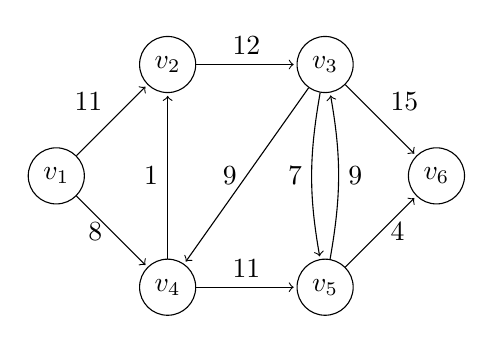
\begin{tikzpicture}[shorten >=1pt,node distance=2cm,on grid,auto]
   \node[circle, draw] (s)  {$v_1$};
   \node[circle, draw] (v1) [above right=of s]  {$v_2$};
   \node[circle, draw] (v2) [right=of v1]       {$v_3$};
   \node[circle, draw] (v3) [below right=of s]  {$v_4$};
   \node[circle, draw] (v4) [right=of v3]       {$v_5$};
   \node[circle, draw] (t)  [above right=of v4] {$v_6$};
   
   \path[->]
    (s)  edge 				 node        {$11$} (v1)
         edge 				 node[left]  {$8$}  (v3)
    (v1) edge 				 node        {$12$} (v2)
    (v2) edge 				 node        {$15$} (t)
         edge 				 node[left]  {$9$}  (v3)
         edge[bend right=10] node[left]  {$7$}  (v4)
    (v3) edge 				 node        {$1$}  (v1)
         edge 				 node        {$11$} (v4)
    (v4) edge[bend right=10] node[right] {$9$}  (v2)
         edge 				 node[right] {$4$}  (t);
\end{tikzpicture}\\


\definition{Paths}
A \textit{Path} in a graph is a sequence of nodes which are connected by a sequence of edges.\\
\textit{Path}s can be further categorised as
\begin{itemize}
	\item[-] A \textit{Trail} is a \textit{Path} where every vertex within it is only met once.
	\item[-] A \textit{Walk} is a \textit{Path} where every vertex \& edge within it are only traversed once.
	\item[-] A \textit{Cycle} is a \textit{Trail} which starts and ends on the same vertex.
	\item[-] A \textit{Simple Path} is a \textit{Path} which has no repeating edges.
\end{itemize}

\example{Paths}
Consider the graph in \textbf{Example 1.1}.
\begin{itemize}
	\item[-] $v_1\to v_2\to v_3\to v_45$ is a \textit{Simple Path}, a \textit{Trail} \& a \textit{Path}.
	\item[-] $v_2\to v_3\to v_4\to v_2$ is a \textit{Cycle}.\\
\end{itemize}

\definition{Connected Graph}
A \textit{Connected Graph} is a graph in which there exists at least one path between each pair of vertices.\\
If there exists one pair of edges which a path cannot be formed between, then the graph is said to be \textit{disconnected}.\\

\definition{Bridge}
A \textit{Bridge} is an edge of a connected graph which, if it was deleted, would leave the graph disconnected.\\

\newpage
\example{Connected Graph \& Bridge Edge}
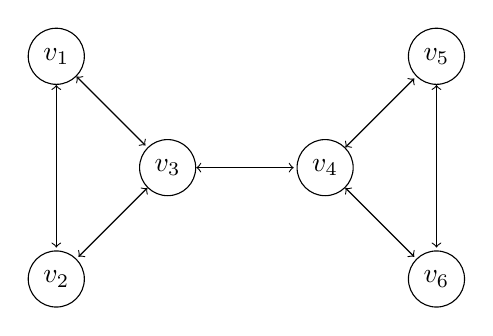
\begin{tikzpicture}[shorten >=1pt,node distance=2cm,on grid,auto]
   \node[circle, draw] (v1) {$v_1$};
   \node[circle, draw] (v3) [below right=of v1]  {$v_3$};
   \node[circle, draw] (v2) [below left =of v3]  {$v_2$};
   \node[circle, draw] (v4) [right=of v3]        {$v_4$};
   \node[circle, draw] (v5) [above right=of v4]  {$v_5$};
   \node[circle, draw] (v6) [below right=of v4]  {$v_6$};
   
   \path[<->]
    (v1) edge (v2)
         edge (v3)
    (v3) edge (v2)
         edge (v4)
    (v4) edge (v5)
         edge (v6)
    (v5) edge (v6);
\end{tikzpicture}\\
\nb The edge $(v_3,v_4)$ is a bridge.\\

\definition{Bipartite Graphs}
\textit{Bipartite Graph} is a graph where its vertices can be divided into independent disjoint sets such that every edge connects a vertex from one set, to a vertex in the other.\\

\example{Bipartite Graph}
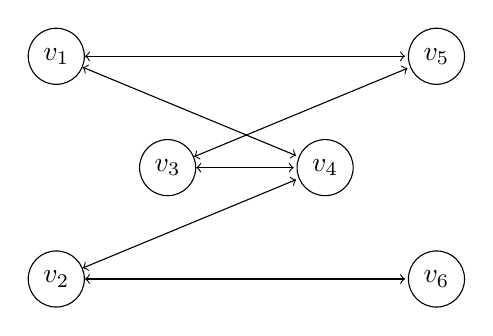
\begin{tikzpicture}[shorten >=1pt,node distance=2cm,on grid,auto]
   \node[circle, draw] (v1) {$v_1$};
   \node[circle, draw] (v3) [below right=of v1]  {$v_3$};
   \node[circle, draw] (v2) [below left =of v3]  {$v_2$};
   \node[circle, draw] (v4) [right=of v3]        {$v_4$};
   \node[circle, draw] (v5) [above right=of v4]  {$v_5$};
   \node[circle, draw] (v6) [below right=of v4]  {$v_6$};
   
   \path[<->]
    (v1) edge (v4)
         edge (v5)
    (v3) edge (v4)
         edge (v5)
    (v2) edge (v4)
         edge (v6);
\end{tikzpicture}\\
This graph can be split into $[v_1, v_2, v_3]$ \& $[v_4, v_5, v_6]$ to be a bipartite graph.\\

\definition{Node Degree}
The \textit{Degree} of a node in an \textit{undirected graph} is the number of edges connected to that node.\\
The \textit{Degree} of a node in an \textit{directed graph} is the number of edges into the node less the number of edges leaving it.\\

\proposition{Representing Graphs as Matrices}
A directed graph with $|V|$ vertices can be represented by a $|V|\times|V|$ matrix, $A$.\footnote{See \ttfamily{programs\textbackslash MatrixGraph.java}}\\
Where the value of $A_{ij}$ gives the weight of the edge from $i\to j$.\\
If the value of $A_{ij}$ is $0$ then there is no edge between vertex $i$ \& vertex $j$.\\
If the graph is unweighted then the value of $A_{ij}$ doesn't matter as long as it is not zero.\\

\proposition{Representing Graphs as Adjacency Lists}
Graphs can be represented by an \textit{Adjacency List}.\footnote{See \ttfamily{programs\textbackslash LinkedGraph.java}}\\
An \textit{Adjacency List} can be represented by a map from a vertex to a linked list.\\
The linked list stores the vertices that the vertex has an edge to and the weight of that edge as tuples.\\

\remark{Comparison of Graph Representations}
Let $|V|$ be the number of vertices \& $|E|$ be the number of edges in a Graph.\\
\begin{tabular}{|c|c|c|c|}
\hline
&Space&Is there an edge $i\to j$&Get all edges leaving $i$\\
\hline
Matrix&$\Theta(|V|^2)$&$O(1)$ Time& $O(|V|)$ Time\\
Adjacency List&$\Theta(|V|+|E|)$& O($degree(i)$) Time& O($degree(i)$) Time\\
\hline
\end{tabular}\\
\nb Adjacency lists take up a lot of space when loaded into memory.\\

\definition{Tree}
A \textit{Tree} is an undirected graph where each node can be connected by exactly one path.\\

\definition{Binary Tree}
A \textit{Binary Tree} is a tree where each node has either $0$, $1$ or $2$ children.\\

\example{Binary Tree}
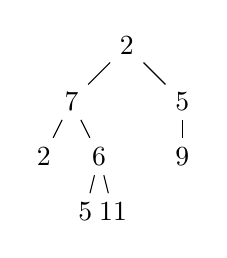
\begin{tikzpicture}[level distance=2em, sibling distance=4em, level 2/.style={sibling distance=2em}, level 3/.style={sibling distance=1em}]
  \node {2}
    child { node {7} 
    	child {node {2} }
    	child {node {6} 
    		child {node {5} }
    		child {node {11} }
    		}
    	}
    child { node {5} 
    	child {node {9} }
    };
\end{tikzpicture}

\definition{Balance}
A tree is said to be \textit{Balanced} if the heights of the left \& right subtrees of all vertices differ by no more than one.\\

\definition{Binary Tree Rotation}
A \textit{Rotation} is an operation on a binary tree that changes the structures of the tree without affect the order of elements.\\
They are used to balance trees so that they are as short as possible and thus quick to search.\\
\nb The vertex we balance around is called the \textit{pivot}.\\

\definition{Left Rotation}
A \textit{Left Rotation} can be used to balance a binary tree if the left subtree of a given node causes an imbalance at that node.\\
A \textit{Left Rotation} can be performed by the following process
\begin{enumerate}
	\item Remove the pivot's left subtree.
	\item Make the parent, and its left subtree, the pivot's righleft child.
	\item Make the removed subtree the right child of the old parent.
\end{enumerate}

\example{Left Rotation}
Here we shall perform a left rotation on the following tree.\\
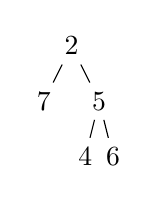
\begin{tikzpicture}[level distance=2em, sibling distance=2em, level 2/.style={sibling distance=1em}]
  \node {2}
    child { node {7} }
    child { node {5} 
        child {node {4} }
    	child {node {6} }
    };
\end{tikzpicture}\\
To do so we must pivot around 5.\\
Left child.\\
\begin{tikzpicture}[level distance=2em, sibling distance=2em, level 2/.style={sibling distance=1em}]
  \node {4};
\end{tikzpicture}\\
Parent and its left child.\\
\begin{tikzpicture}[level distance=2em, sibling distance=2em, level 2/.style={sibling distance=1em}]
  \node {2}
    child { node {7} };
\end{tikzpicture}\\
Pivot and its right child.\\
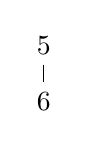
\begin{tikzpicture}[level distance=2em, sibling distance=2em, level 2/.style={sibling distance=1em}]
  \node {5}
    child { node {6} }; 
\end{tikzpicture}\\
\newpage
Make parent the pivot's right child.\\
\begin{tikzpicture}[level distance=2em, sibling distance=2em, level 2/.style={sibling distance=1em}]
  \node {5}
    child { node {2} 
    	child {node {7} }
    	}
    child { node {6} };
\end{tikzpicture}\\
Make the removed child the parent's left child.\\
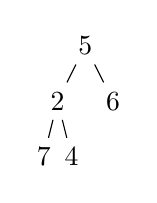
\begin{tikzpicture}[level distance=2em, sibling distance=2em, level 2/.style={sibling distance=1em}]
  \node {5}
    child { node {2} 
    	child {node {7} }
    	child {node {4} }
    	}
    child { node {6} };
\end{tikzpicture}

\definition{Right Rotation}
A \textit{Right Rotation} is used to balance a binary tree if the left subtree of a node is taller than the right.\\
A \textit{Right Rotation} can be performed by the following process
\begin{enumerate}
	\item Remove the pivot's right subtree.
	\item Make the parent, and its right subtree, the pivot's right child.
	\item Make the removed subtree the left child of the old parent.
\end{enumerate}


\example{Right Rotation}
Here we shall perform a right rotation on the following tree.\\
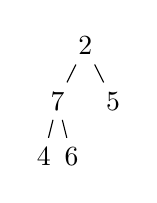
\begin{tikzpicture}[level distance=2em, sibling distance=2em, level 2/.style={sibling distance=1em}]
  \node {2}
    child { node {7} 
    	child {node {4} }
    	child {node {6} }
    	}
    child { node {5} };
\end{tikzpicture}\\
To do so we must pivot around 7.\\
Right child.\\\begin{tikzpicture}[level distance=2em, sibling distance=2em, level 2/.style={sibling distance=1em}]
  \node {6};
\end{tikzpicture}\\
Parent and its left child.\\
\begin{tikzpicture}[level distance=2em, sibling distance=2em, level 2/.style={sibling distance=1em}]
  \node {2}
    child { node {5} };
\end{tikzpicture}\\
Pivot and its left child.\\
\begin{tikzpicture}[level distance=2em, sibling distance=2em, level 2/.style={sibling distance=1em}]
  \node {7}
    child { node {4} }; 
\end{tikzpicture}\\
Make parent the pivot's right child.\\
\begin{tikzpicture}[level distance=2em, sibling distance=2em, level 2/.style={sibling distance=1em}]
  \node {7}
    child { node {4} }
    child { node {2} 
    	child {node {5} }
    };
\end{tikzpicture}\\
Make the removed child the parent's left child.\\
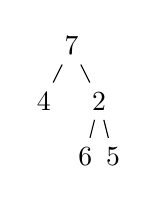
\begin{tikzpicture}[level distance=2em, sibling distance=2em, level 2/.style={sibling distance=1em}]
  \node {7}
    child { node {4} }
    child { node {2} 
    	child {node {6} }
    	child {node {5} }
    	};
\end{tikzpicture}

\definition{Complete Binary Tree}
A \textit{Complete Binary Tree} is a binary tree where every layer is full, except for the bottom layer.\\

\example{Complete Binary Tree}
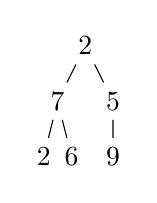
\begin{tikzpicture}[level distance=2em, sibling distance=2em, level 2/.style={sibling distance=1em}]
  \node {2}
    child { node {7} 
    	child {node {2} }
    	child {node {6} }
    	}
    child { node {5} 
    	child {node {9} }
    };
\end{tikzpicture}

\definition{Binary Heap}
A \textit{Binary Heap} is a complete binary tree which satisfies a heap ordering property.\\
There are two heap ordering properties
\begin{enumerate}[label=\roman*)]
	\item \textit{Min-Heap Property} - The value of each node is greater than, or equal to, its parent.
	\item \textit{Max-Heap Property} - The value of each node is less than, or equal to, its parent.
\end{enumerate}

\example{Binary Heap}
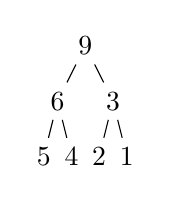
\begin{tikzpicture}[level distance=2em, sibling distance=2em, level 2/.style={sibling distance=1em}]
  \node {9}
    child { node {6} 
    	child {node {5} }
    	child {node {4} }
    	}
    child { node {3} 
    	child {node {2} }
    	child {node {1} }
    };
\end{tikzpicture}
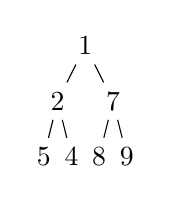
\begin{tikzpicture}[level distance=2em, sibling distance=2em, level 2/.style={sibling distance=1em}]
  \node {1}
    child { node {2} 
    	child {node {5} }
    	child {node {4} }
    	}
    child { node {7} 
    	child {node {8} }
    	child {node {9} }
    };
\end{tikzpicture}

\remark{Implementing Binary Heap - Array}\footnote{See \ttfamily{programs\textbackslash BinaryHeapPriorityQueue.java}}
A \textit{Binary Heap} can be implemented using an array by storing the values layer by layer.\\
This means the $n^{th}$ layer starts at index $2^n-1$.\\
For element $i$ in the list we can get the index of its parent \& children using
\begin{itemize}
  \item[-] $Parent(i) = \big\lfloor\frac{i}{2}\big\rfloor$.
  \item[-] $Left-Child(i) = 2i+1$
  \item[-] $Right-Child(i) = 2i+2$
\end{itemize}

\remark{Finding Elements in Binary Heap}
To store elements in a binary heap, rather than just positive integers, create a lookup table maps a positive integer to a pointer to the element.\\
This assigned value is the element's ID.\\
To find the element with ID $i$, look up the $i^{th}$ element of the lookup table.\\
This will be a pointer to that element.


\subsection{Priority Queue}

\definition{Priority Queue}
A \textit{Priority Queue} is an abstract data type which stores a set of distinct elements.\\
Each element has an associated value, called its \textit{key}.\\
All \textit{Priority Queue}s can perform the following operations.
\begin{enumerate}[label=\roman*)]
  \item $INSERT(x,k)$ - Inserts new element $x$ and sets $x.key=k$.
  \item $DESCREASE-KEY(x,k)$ - Decrease a $x.key$ to equal $k$, where $k<x.key$.
  \item $EXTRACT-MIN()$ - Removes \& returns the element with the smallest value key. When multiple elements have the lowest value, one is returned arbitrarily.
\end{enumerate}

\newpage
\proposition{Implementing Priority Queue - Unsorted Linked-List}
An \textit{Unsorted Linked-List} can be used to implement a priority queue.\\
The operations of a \textit{Priority Queue} can be emulated by
\begin{enumerate}[label=\roman*)]
  \item $INSERT(x,k)\in O(1)$.\\
  Element is placed at the start of the list.
  \item $DESCREASE-KEY(x,k) \in O(n)$.\\
  Increment through the list until $x$ is found.
  \item $EXTRACT-MIN()\in O(n)$.\\
  Increment through the list until $x$ is found.
\end{enumerate}
\nb A coded example of this can be seen in {\ttfamily{programs/UnsortedLinkedPriorityQueue.java}}\\

\proposition{Implementing Priority Queue - Sorted Linked-List}
A \textit{Sorted Linked-List} can be used to implement a priority queue.\\
The operations of a \textit{Priority Queue} can be emulated by
\begin{enumerate}[label=\roman*)]
  \item $INSERT(x,k)\in O(n)$.\\
  Incrementing through the list until you find an element whose key is greater than $k$.\\
  Insert $x$ before this element.
  \item $DESCREASE-KEY(x,k) \in O(n)$.\\
  Increment through the list until you find $x$, decrease its key and move it forward until you encounter an element whose key is less less than $k$.\\
  Place decremented element after this element.
  \item $EXTRACT-MIN()\in O(1)$.\\
  Lowest value element is always are front of list.
\end{enumerate}
\nb A coded example of this can be seen in {\ttfamily{programs\textbackslash SortedLinkedPriorityQueue.java}}\\

\proposition{Implementing Priority Queue - Binary Heap\footnote{See {\ttfamily{programs\textbackslash BinaryHeapPriorityQueue.java}}}}
A \textit{Minimum Binary Heap} can me used to implement a priority queue.\\
The height of the heap is $\lceil\log_2n\rceil$, so this is the maximum number of elements which need to be checked in any operation.\\
Reinstating the heap property of a binary heap is $\in O(\log_2n)$.\\
The operations of a \textit{Priority Queue} can be emulated by
\begin{enumerate}[label=\roman*)]
  \item $INSERT(x,k)\in O(\log_2n)$.\\
  Add the element to the bottom of the heap.\\
  Compare $k$ to the key of the new element's parent, if $k$ is less then swap the nodes.\\
  Repeat this until the parent's key is less than $k$ or you have reached the top of the list.
  \item $DESCREASE-KEY(x,k) \in O(\log_2n)$.\\
  Find $x$ in the heap and update its key.\\
  Compare $k$ to the key of the new element's parent, if $k$ is less then swap the nodes.\\
  Repeat this until the parent's key is less than $k$ or you have reached the top of the list.
  \item $EXTRACT-MIN()\in O(\log_2n)$.\\
  Remove the top element from the heap.\\
  Move the last element of the heap to be the root.\\
  If its left child has a lower key then swap them, else if the right child has a lower key then swap them.\\
  Repeat until both children have a greater key or you have reached the bottom of the list.
\end{enumerate}

\remark{Summary of Priority Queue Implementations}
Here is a summary of the space complexity and run-time complexity for the operations required to implement a priority queue for different data structures.\\
Let $N$ to be the maximum key for element.\\
\begin{tabular}{|l|c|c|c|c|}
\hline
&INSERT&DECREASE-KEY&EXTRACT-MIN&SPACE\\
\hline
Unsorted Linked-List&O(1)&O(n)&O(n)&O(n)\\
Sorted Linked-List&O(n)&O(n)&O(1)&O(n)\\
Binary Heap&O($log_2n$)&O($log_2n$)&O($log_2n$)&O(N)\\
\hline
\end{tabular}\\
\nb Fibonacci heaps are better than binary heaps, however they are complex and generally not practical. (They are not in this course).

\subsection{Disjoint Sets}

\definition{Disjoint Sets}
\textit{Disjoint Sets} is an abstract data structure.\\
It emulates a collection of sets of elements that have no common values between or within them.\\
Each set has a unique identifier, called its \textit{identity}.\\
The \textit{identity} can be implemented in any way.\\
All \textit{Disjoint Sets} can perform the following operations
\begin{enumerate}[label=\roman*)]
  \item $MAKE-SET(x)$ - Makes a new set containing only $x$.
  \item $UNION(x,y)$ - Merges the set containing element $x$ with the set containing element $y$.
  \item $FIND-SET(x)$ - Returns the \textit{identity} of the set contain $x$.
\end{enumerate}

\theorem{Uniqueness of FINDSET(x)}
$FIND-SET(x)\equiv FIND-SET(y)$ iff $x$ and $y$ are in the same set.\\

\remark{Operations of Disjoint Sets enforce Disjointedness}
Two sets cannot have a shared element since first you must call $MAKE-SET(x)$ which will not run if $x$ is already in a set.\\
There is no other way to add elements to disjoint sets.\\

\proposition{Implementation of Disjoint Sets - Reverse Tree}
A collection of \textit{Reverse Trees} can be used to implement disjoint sets.\\
Reverse trees can be stored in an array of fixed length where the index of an element gives the value and the item in that index is a pointer to its parent.\\
You need unique values to distinguish parents \& unused values.\\
The root of each tree is the identity of that set.\\
Children point to parents, but parents do not point to children.\\
The operations of \textit{Disjoint Sets} can be emulated by
\begin{enumerate}[label=\roman*)]
	\item $MAKE-SET(x)\in O(1)$.\\
	Expand array to accommodate $x$.\\
	Set $x$ to be a parent.
	\item $UNION(x,y)\in O(tree-height)$\\
	Set $r_x=FIND-SET(x)$ \& $r_y=FIND-SET(y)$.\\
	Point $r_y$ to $r_x$.
	\newpage
	\item $FIND-SET(x)\in O(tree-height)$.\\
	Find the pointer in index $x$.\\
	Follow its pointer to the next element.\\
	Repeat this until the pointer indicates the element is a parent.\\
	Return the index of this pointer
\end{enumerate}
\nb A coded example of this can be seen in {\ttfamily{programs/ReverseTreeDisjointSets.java}}.\\

\proposition{Height of Reverse Tree}
In the worst case implementation of $UNION(x,y)$ the tree height will increase by one every time, causing all operations to run in $O(n)$.\\
This can improved by balancing the trees.\\
One way is to store the heights of the trees and always making the shorter tree the child of the other.\\
By doing this, the height of the resulting tree only increases, by one, if the two previous trees were the same height.\\
\nb This is the version implemented in {\ttfamily{programs/ReverseTreeDisjointSets.java}}.\\

\proof{The height of the tallest tree is $log_2n$}
Here we shall prove that by using the previously described process the tallest resulting trees will have height $log_2n$.\\
\textit{This is a proof by contradiction}.\\
We begin by proving that any tree of height $h$ contains at least $2^h$ nodes.\\
\textit{This is a proof by induction}.\\
\textit{Base Case}\\
Set $i=0$.\\
A tree of height $0$ is a single node. $2^i=2^0=1$.\\
The claim holds.\\
\textit{Inductive Step}\\
Assume that every tree of height $i-1$ contains at least $2^{i-1}$ nodes.\\
$UNION(x,y)$ only produces a tree of height $i$ when passed two trees of height $i-1$.\\
Therefore, a tree of height $i$ contains $2^{i-1}+2^{i-1}=2.2^{i-1}=2^i$ nodes.\\
Now assume, for contradiction, that there is a tree of height $h\geq\log_2n+1$.\\
This tree contains at least $2^{log_2n+1}$, which is greater than $n$, nodes and each node represents a distinct element.\\
This is a contradiction because the elements are members of the set $\{1,2,\dots,n\}$ so $h\leq\log_2n$.

\subsection{Spanning Trees}

\definition{Spanning Tree}
A \textit{Spanning Tree} is a sub-graph of a connected, undirected graph that contains every element of the graph and has no cycles.\\

\definition{Weight of Spanning Tree}
The \textit{weight} of a spanning tree is the sum of the weights of its edges.\\

\definition{Minimum Spanning Tree}
A \textit{Minimum Spanning Tree} of a given graph is the spanning tree with the lowest weight.\\

\newpage
\example{Minimum Spanning Tree}
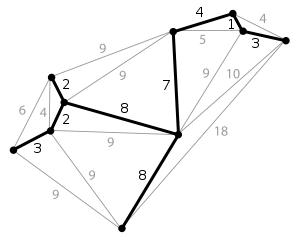
\includegraphics[scale=0.4]{minimumSpanningTree}

\remark{Finding Minimum Spanning Trees}
\textit{Kruskal's Algorithm} can be used to find minimum spanning trees\footnote{See  \textbf{Subsection 3.9}}.

\subsection{Dynamic Search Structures}

\definition{Dynamic Search Structures}
A \textit{Dynamic Search Structure} stores a set of elements.\\
Each element $x$ has a unique key, $x.key$.\\
All \textit{Dynamic Search Structure}s can perform the following operations 
\begin{enumerate}[label=\roman*)]
  \item $INSERT(x,k)$ - Inserts element $x$ with key $k$.
  \item $FIND(k)$ - Returns the unique element $x$ where $x.key\equiv k$.
  \item $DELETE(k)$ - Deletes the unique element $x$ where $x.key\equiv k$.
\end{enumerate}

\remark{Addition Operations of Dynamic Search Structures}
The following are additional operations which are useful for \textit{Dynamic Search Structures} to support
\begin{enumerate}[label=\roman*)]
  \item $PREDECESSOR(k)$ - returns the unique element $x$ with the largest key st $x.key<k$.
  \item $RANGE-FIND(k_1,k_2)$ - returns every element $x$ where $k_1\leq x.key\leq k_2$.
\end{enumerate}

\remark{Usefulness of PREDECESSOR}
$PREDECESSOR$ is used when deleting elements from structures with heap properties as replacing an element with its predecessor ensures the heap property is maintained.\\

\proposition{Implementing Dynamic Search Structure - Unsorted Linked List}
An \textit{unsorted linked list} is a valid data structure to implement as a dynamic search structure.\\
The run-time complexity for the operations is
\begin{enumerate}[label=\roman*)]
  \item $INSERT\in O(1)$.
  \item $FIND\in O(n)$.
  \item $DELETE\in O(n)$.
\end{enumerate}
where $n$ is the number of elements in the linked list.\\

\newpage
\proposition{Implementing Dynamic Search Structure - Binary Search Tree}
A \textit{Binary Search Tree} is a valid data structure to implement as a dynamic search structure.\footnote{See {\ttfamily{programs\textbackslash BinarySearchTree.java}}}\\
The operations can be implemented as follows
\begin{enumerate}[label=\roman*)]
  \item $INSERT(x,k)\in O(h)$.\\
  Traverse down the tree comparing node keys to $k$.\\
  If a node's key $=k$ throw an error saying the key is not unique.\\
  If a node's key $> k$ follow its left subtree.\\\
  If a node's key $<k$ follow its right subtree.\\
  If a node does not have a required subtree, insert the element as a leaf there.
  \item $FIND(k)\in O(h)$.\\
  Traverse down the tree comparing node keys to $k$.\\
  If a node's key $=k$ return the associated element.\\
  If a node's key $>k$ follow its left subtree.\\\
  If a node's key $<k$ follow its right subtree.\\
  Add new key and element as a child to leaf.  
  \item $DELETE(k)\in O(h)$.\\
  Traverse down the tree, if you reach a leaf that is not the desired key return FAIL.\\
  When key is found
  \begin{enumerate}
  	\item If node has no children, delete node.
  	\item If node only has left subtree, delete node \& replace with left child.
  	\item If node only has right subtree, delete node \& replace with right child.
  	\item If node has both children, find its predecessor and replace node with it.
  \end{enumerate}
\end{enumerate}
where $h$ is the height of the tree.\\
\nb $h\geq\log_2n$.\\

\proposition{Implementing Dynamic Search Structure - 2-3-4 Tree}
A \textit{2-3-4 Tree}\footnote{See \textbf{Definition 6.3}} is a valid data structure to implement as a dynamic search structure.\footnote{See {\ttfamily{programs\textbackslash Tree234.java}}}\\
The operations can be implemented as follows
\begin{enumerate}[label=\roman*)]
	\item $INSERT(x,k)\in O(h)\equiv O(\log_2n)4$.\\
	Traverse down the tree, comparing node keys to $k$.\\	
	Whenever you encounter a $4\ node$ perform $SPLIT$ on it.\\
	If a node contains $k$ as a key, throw an error saying $k$ is not unique.\\
	Otherwise, follow the subtree which $k$ is bounded on.\\		
	If you reach a leaf, insert the value by
	\begin{enumerate}
	  \item If leaf is $2\ node$ convert to $3\ node$ with the new key, $k$.
	  \item If leaf is $3\ node$ convert to $4\ node$ with the new key, $k$.
	\end{enumerate}
	\item $FIND(k)\in O(h)\equiv O(\log_2n)$.\\
	Traverse down the tree, comparing node keys to $k$.\\
	\quad Whenever you encounter a $4\ node$ perform $SPLIT$ on it.\\
	If a node contains $k$ as a key, return it.\\
	Otherwise, follow the subtree which $k$ is bounded on.\\
	If you reach a node without the appropriate child, return FAIL.
	\item $DELETE(k)\in O(h)\equiv O(\log_2n)$.\\
	Traverse down the tree, comparing node keys to $k$.\\
	Whenever you encounter a $2\ node$ perform $FUSE$ or $TRANSFER$ on it.\\
	If a node does not contain $k$ as a key, follow the subtree which $k$ is bounded on.\\
	If you reach a leaf and it doesn't contain $k$ as a key, throw an error saying key is unused.\\
	Otherwise
	\begin{enumerate}
	  \item Search for key $k$ using $FIND(k)$. Perform $FUSE$ or $TRANSFER$ on all $2\ node$s met here.
	  \item If node is a leaf \&\& a $3\ node$ remove key and downgrade to $2\ node$.
	  \item If node is a leaf \&\& a $4\ node$ remove key and downgrade to $3\ node$.
	  \item If node is \textbf{not} a leaf:
	  \begin{enumerate}
    	\item Use $PREDECESSOR(k)$ to find a leaf $k'$.
	    \item Perform $DELETE(k')$.
	    \item Overwrite $k$ with $k'$.
	  \end{enumerate}
	\end{enumerate}
\end{enumerate}
\nb By performing $SPLIT$ on all met $4\ node$s, we will never end up trying to add the new key to a $4\ node$.\\
\nb By performing $FUSE$ or $TRANSFER$ on all met $2\ node$s, we will never end up trying to delete a key from a $2\ node$.\\

\proposition{Implementing Dynamic Search Structure - Skip List}
A \textit{Skip List}\footnote{See \textbf{Definition 7.2}} is a valid data structure to implement as a dynamic search structure.\footnote{See {\ttfamily{programs\textbackslash SkipList.java}}}\\
The operations can be implemented as follows
\begin{enumerate}
	\item $INSERT(x,k)\in O(\log_2n)$ on average.\footnote{See \addtocounter{proposition}{2}\textbf{Proposition \arabic{subsection}.\arabic{proposition}}\addtocounter{proposition}{-2}}\\
	Start at the first element of the top level.\\
	Move along the level until you find $k'>k$.\\
	Move down a level at the key directly before $k'$.\\
	Repeat moving along and down until you reach the bottom level.\\
	Move along bottom level until you find $k'>k$.\\
	Insert $(x,k)$ directly before $k'$.
	Repeatedly flip a coin
	\begin{enumerate}
		\item HEADS - Insert $(x,k)$ into the level above.
		\item TAILS- stop.
	\end{enumerate}
	\item $FIND(k)\in O(\log_2n)$ on average.\footnote{See \addtocounter{proposition}{2}\textbf{Proposition \arabic{subsection}.\arabic{proposition}}\addtocounter{proposition}{-2}}\\
	Start at the first element of the top level.\\
	Move  along level until you find $k'>k$.\\
	Move down a level at the key directly before $k'$.\\
	Repeat moving along and down until you reach the bottom level.\\
	Move along bottom level until you find $k'>k$.\\
	Move along the bottom level.\\
	If you find $k$ return the associated element.\\
	If you find $k'>k$ return FAIL.
	\newpage
	\item $DELETE(k)\in O(\log_2n)$ on average.\footnote{See \addtocounter{proposition}{2}\textbf{Proposition \arabic{subsection}.\arabic{proposition}}\addtocounter{proposition}{-2}}\\
	Perform $FIND(k)$.\\
	If this fails, return FAIL.\\
	Otherwise, delete $(x,k)$ from all layers.
\end{enumerate}

\theorem{The Union Bound Theorem}
Let $E_1,E_2,\dots,E_n$ be events where the probabilty of $E_j$ occuring is $p_j$.\\
Then the probability of at least one of $E_1,\dots,E_j$ occuring is at most $\sum_{i=1}^jp_i$.\\

\remark{Run-Time Complexity for Skip List Operations}
\textit{Skip Lists} having a randomised algorithm for their construction.\\
The run-time complexity depends on the number of levels.\\
Thus run-time complexity for all their operations is given for the average case.\\

\proposition{Run-Time Complexity of FIND with a Skip List}
Since the number of levels is $O(\log_2n)$ we can conclude that the number of times we move \textit{down} the skip list is $O(\log_2n)$.\\
For any given element, in any level, the probability of the element to its immediate right is also being the element to its immediate right in the bottom layer is $\frac{1}{2}$.\\
We can conclude that we are likely to move right $O(\log_2n)$ times.\\
Since each movement has run-time complexity $\in O(1)$ we conclude that $FIND\in O(\log_2n)$.\\

\remark{Comparing Implementations of Dynamic Search Structures}
Let $n$ be the number of elements being stored.\\
\begin{tabular}{|c|c|c|c|c|}
  \hline
  &$INSERT(x,k)$&$DELETE(k)$&$FIND(k)$&Space\\
  \hline
  Unsorted Linked List & $O(1)$ & $O(n)$ & $O(n)$ & $O(n)$\\
  \hline
  Binary Search Tree & $O(n)$ & $O(n)$ & $O(n)$ & $O(n)$\\
  \hline
  2-3-4 Tree & $O(\log_2n)$ & $O(\log_2n)$ & $O(\log_2n)$ & $O(n)$\\
  \hline
  Red-Black Tree & $O(\log_2n)$ & $O(\log_2n)$ & $O(\log_2n)$ & $O(n)$\\
  \hline
  Skip List & $O(\log_2n)$ & $O(\log_2n)$ & $O(\log_2n)$ & $O(n)$\\
  \hline
\end{tabular}

\subsection{Self-Balancing Trees}

\definition{Prefect Balance}
A tree has \textit{Perfect Balance} if the length of every path from the root to any leaf is exactly the same as the height of the tree.\\

\definition{Self-Balancing Trees}
A \textit{Self-Balancing Tree} automatic ensures perfect balance when inserting or deleting elements.\\

\newpage
\definition{2-3-4 Tree}
A \textit{2-3-4 Tree} is a tree where all nodes have $0, 2, 3$ or $4$ children only.\\
The nodes are named as
\begin{itemize}
  \item[-] $2\ node$ which have 2 children \& 1 key.
  \item[-] $3\ node$ which have 3 children \& 2 keys.
  \item[-] $2\ node$ which have 4 children \& 3 keys.
\end{itemize}
A \textit{2-3-4 Tree} can implemented as a \textit{Dynamic Search Structure}.\footnote{See \ttfamily{programs\textbackslash Tree234.java}}\\
\nb Each node has either the specified number of children or none.\\

\remark{Why 2-3-4?}
By seeing the efficiencies of a \textit{2-3-4 Tree} we may consider why we don't use a \textit{2-3-$\dots$-n Tree}.\\
This is because the more children a node has, the flatter the tree becomes and the more nodes we have to deal with at each level, rather than just moving down sub-trees.\\
It seems \textit{2-3-4 Tree} maximises these efficiencies.\\

\remark{Height of $2-3-4$ Tree}
The height, $h$, of a $2-3-4$ tree is $\log_4n\leq h\leq\log_2n$.\\
This boundaries represent the case where all the nodes are $4\ nodes$ and the case where all the nodes are $2\ nodes$.\\

\definition{2 Node}
A $2\ node$ has a single key and two sub-trees.\\
All the elements in the left sub-tree have a value less than the key,\\
and all those in the right sub-tree have a value greater than the key.\\

\example{2 Node}
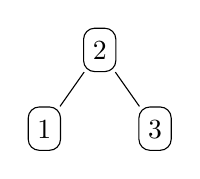
\begin{tikzpicture}[node distance = 2cm, auto, level distance=10mm, text depth=.1em, text height=.8em, level 1/.style={sibling distance=4em}, level 2/.style={sibling distance=2em}]
  \node[rectangle, draw, rounded corners] {2}
    child {node[rectangle, draw, rounded corners] {1}}
    child {node[rectangle, draw, rounded corners] {3}};
\end{tikzpicture}\\

\definition{3 Node}
A $3\ node$ has two keys and three sub-trees.\\
Let $x,y$ be the values of the keys st $x<y$.\\
All the elements in the left sub-tree have a value $<x$.\\
All the elements in the middle sub-tree have a value $>x$ AND $<y$.\\
All the elements in the right sub-tree have a values $>y$.\\

\example{3 Node}
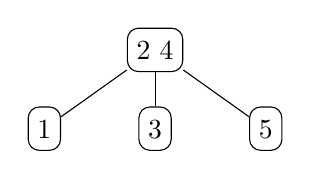
\begin{tikzpicture}[node distance = 2cm, auto, level distance=10mm, text depth=.1em, text height=.8em, level 1/.style={sibling distance=4em}, level 2/.style={sibling distance=2em}]
  \node[rectangle, draw, rounded corners] {2 4}
    child {node[rectangle, draw, rounded corners] {1}}
    child {node[rectangle, draw, rounded corners] {3}}
    child {node[rectangle, draw, rounded corners] {5}};
\end{tikzpicture}\\

\newpage
\definition{4 node}
A $4\ node$ has three keys and four sub-trees.\\
Let $x,y,z$ be the values of the keys st $x<y<z$.\\
All the elements in the left subtree have a value $<x$.\\
All the elements in the middle-left subtree have a value $>x$ AND $<y$.\\
All the elements in the middle-right subtree have a value $>y$ AND $<z$.\\
All the elements in the right subtree have a value $>z$.\\

\example{4 Node}
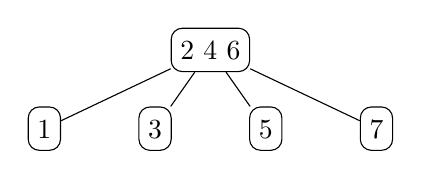
\begin{tikzpicture}[node distance = 2cm, auto, level distance=10mm, text depth=.1em, text height=.8em, level 1/.style={sibling distance=4em}, level 2/.style={sibling distance=2em}]
  \node[rectangle, draw, rounded corners] {2 4 6}
    child {node[rectangle, draw, rounded corners] {1}}
    child {node[rectangle, draw, rounded corners] {3}}
    child {node[rectangle, draw, rounded corners] {5}}
    child {node[rectangle, draw, rounded corners] {7}};
\end{tikzpicture}\\

\proposition{Inserting Elements into 2-3-4 Tree}
To insert a new element to a \textit{2-3-4 Tree} traverse down the tree, following the correct path.\\
Whenever you encounter a $4\ node$, split it and continue traversing.\\
Once you reach a leaf insert the value into the node.\\

\proposition{Deleting Leaf from 2-3-4 Tree}
To delete a value from a leaf first traverse down the tree to the leaf.\\
If the leaf is a $2\ node$ transfer or fuse it with a neighbour.\\
Remove the element as a key from the leaf.\\

\proposition{Deleting from Node in 2-3-4 Tree}
To delete a value from a node first traverse to the node.\\
Find the predecessor to the value you are trying to delete.\\
Delete the predecessor from the tree.\\
Replace the value you are deleting with its predecessor.\\

\definition{Splitting 4 Nodes}
We can \textit{split} any $4\ node$ into two $2\ node$s, provided the $4\ node$'s parent is not a $4\ node$ (otherwise the parent would have too many children).\\
Let $n$ be a $4\ node$ and $p$ be its parent.\\
We can split $n$ using the following process
\begin{enumerate}
  \item Move the middle key of $n$ to the appropriate place in $p$'s keys.
  \item Make a new $2\ node$ using the lesser of the two remaining keys of $n$ \& the two leftmost subtrees of $n$.
  \item Make another new $2\ node$ using the remaining key \& subtrees of $n$.
  \item Make these two new $2\ node$s children of $p$, ensuring numerical order is maintained.
\end{enumerate}
\nb Splitting a node does not affect the height of the tree.\\

\example{Splitting 4 Node}
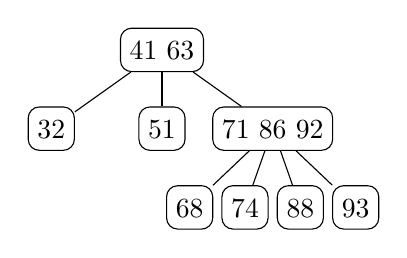
\begin{tikzpicture}[node distance = 2cm, auto, level distance=10mm, text depth=.1em, text height=.8em, level 1/.style={sibling distance=4em}, level 2/.style={sibling distance=2em}, baseline=(current bounding box.center)]
  \node[rectangle, draw, rounded corners] {41 63}
    child {node[rectangle, draw, rounded corners] {32}}
    child {node[rectangle, draw, rounded corners] {51}}
    child {node[rectangle, draw, rounded corners] {71 86 92}
      child {node[rectangle, draw, rounded corners] {68}}
      child {node[rectangle, draw, rounded corners] {74}}
      child {node[rectangle, draw, rounded corners] {88}}
      child {node[rectangle, draw, rounded corners] {93}}
    };
\end{tikzpicture}
splits to
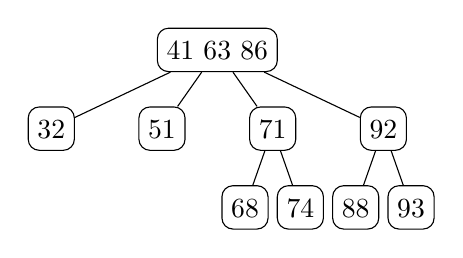
\begin{tikzpicture}[node distance = 2cm, auto, level distance=10mm, text depth=.1em, text height=.8em, level 1/.style={sibling distance=4em}, level 2/.style={sibling distance=2em}, baseline=(current bounding box.center)]
  \node[rectangle, draw, rounded corners] {41 63 86}
    child {node[rectangle, draw, rounded corners] {32}}
    child {node[rectangle, draw, rounded corners] {51}}
    child {node[rectangle, draw, rounded corners] {71}
      child {node[rectangle, draw, rounded corners] {68}}
      child {node[rectangle, draw, rounded corners] {74}}
    }
    child {node[rectangle, draw, rounded corners] {92}
      child {node[rectangle, draw, rounded corners] {88}}
      child {node[rectangle, draw, rounded corners] {93}}
    };
\end{tikzpicture}\\\\

\definition{Splitting the Root}
Since the root doesn't have a parent we do not need to consider the restrictions on splitting it.\\
hen splitting a $4\ node$ root we create a new $2\ node$ root above it.\\
Let $n$ be the root.\\
We can split $n$ using the following process
\begin{enumerate}
	\item Make a new $2\ node$ with the least value of $n$ and its two leftmost subtrees.
	\item Make another new $2\ node$ with the greatest value of $n$ and its two rightmost subtrees.
	\item Make a final $2\ node$ with the middle value of $n$.
	\item Make the other new nodes the children of the last, ensuring numerical order is maintained.
\end{enumerate}
\nb Splitting the root increases the height of the tree by $1$.\\
\nb This has run-time complexity $\in O(1)$.\\

\example{Splitting the Root}
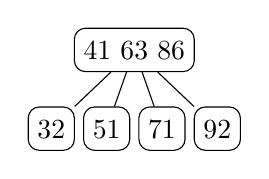
\begin{tikzpicture}[node distance = 2cm, auto, level distance=10mm, text depth=.1em, text height=.8em, level 1/.style={sibling distance=2em}, baseline=(current bounding box.center)]
  \node[rectangle, draw, rounded corners] {41 63 86}
    child {node[rectangle, draw, rounded corners] {32}}
    child {node[rectangle, draw, rounded corners] {51}}
    child {node[rectangle, draw, rounded corners] {71}}
    child {node[rectangle, draw, rounded corners] {92}};
\end{tikzpicture}splits to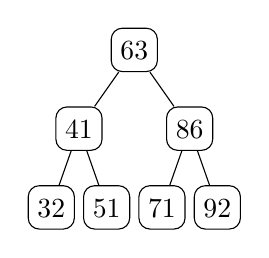
\begin{tikzpicture}[node distance = 2cm, auto, level distance=10mm, text depth=.1em, text height=.8em, level 1/.style={sibling distance=4em}, level 2/.style={sibling distance=2em}, baseline=(current bounding box.center)]
  \node[rectangle, draw, rounded corners] {63}
    child {node[rectangle, draw, rounded corners] {41}
      child {node[rectangle, draw, rounded corners] {32}}
      child {node[rectangle, draw, rounded corners] {51}}
    }
    child {node[rectangle, draw, rounded corners] {86}
      child {node[rectangle, draw, rounded corners] {71}}
      child {node[rectangle, draw, rounded corners] {92}}
    };
\end{tikzpicture}\\\\

\definition{Fusing Two $2\ nodes$}
We can \textit{fuse} two $2\ node$ siblings into a single $4\ node$, provided their parent is not a $2\ node$.\\
Fusing runs in constant time.\\
Let $n_1$ and $n_2$ be $2\ node$ siblings and $p$ be their parent.\\
We can \textit{fuse} $n_1$ \& $n_2$ with $n_1<n_2$ using the following process
\begin{enumerate}
  \item Remove the key of $p$ which forms the boundary between $n_1$ and $n_2$.
  \item Create a new $4\ node$ with the keys of $n_1$, $n_2$ and the key which was just removed from $p$, ensuring order is kept.
  \item Make the sub-trees of $n_1$ the two leftmost sub-trees of the new node, and the sub-trees of $n_2$ as the two rightmost sub-trees of the new node.
\end{enumerate}
\nb Fusing does not affect the height of the tree.\\

\example{Fusing Two $2\ nodes$}
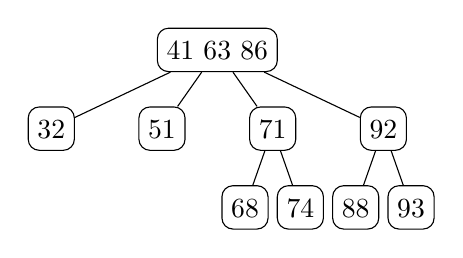
\begin{tikzpicture}[node distance = 2cm, auto, level distance=10mm, text depth=.1em, text height=.8em, level 1/.style={sibling distance=4em}, level 2/.style={sibling distance=2em},  baseline=(current bounding box.center)]
  \node[rectangle, draw, rounded corners] {41 63 86}
    child {node[rectangle, draw, rounded corners] {32}}
    child {node[rectangle, draw, rounded corners] {51}}
    child {node[rectangle, draw, rounded corners] {71}
      child {node[rectangle, draw, rounded corners] {68}}
      child {node[rectangle, draw, rounded corners] {74}}
    }
    child {node[rectangle, draw, rounded corners] {92}
      child {node[rectangle, draw, rounded corners] {88}}
      child {node[rectangle, draw, rounded corners] {93}}
    };
\end{tikzpicture}
fuses to
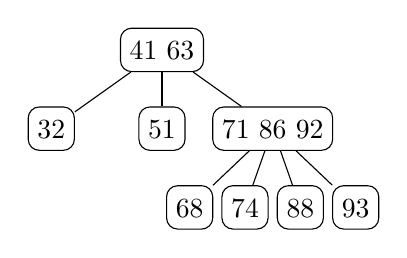
\begin{tikzpicture}[node distance = 2cm, auto, level distance=10mm, text depth=.1em, text height=.8em, level 1/.style={sibling distance=4em}, level 2/.style={sibling distance=2em},  baseline=(current bounding box.center)]
  \node[rectangle, draw, rounded corners] {41 63}
    child {node[rectangle, draw, rounded corners] {32}}
    child {node[rectangle, draw, rounded corners] {51}}
    child {node[rectangle, draw, rounded corners] {71 86 92}
      child {node[rectangle, draw, rounded corners] {68}}
      child {node[rectangle, draw, rounded corners] {74}}
      child {node[rectangle, draw, rounded corners] {88}}
      child {node[rectangle, draw, rounded corners] {93}}
    };
\end{tikzpicture}\\\\

\newpage
\definition{Fusing when parent is the Root}
We said you cannot fuse two nodes if their parent is a $2\ node$, an exception is made for when the parent is the root.\\
Here the root key is brought down to the two children.\\
Let $n_1$ and $n_2$ be the two $2\ nodes$ siblings, whose parent is the root.\\
We can fuse $n_1$ \& $n_2$ with $n_1<n_2$ using the following process
\begin{enumerate}
	\item Create a new $3\ node$ using the keys of $n_1,\ n_2$ \& the root.
	\item Make the children of $n_1$ the leftmost children of the new node.
	\item Make the children of $n_2$ the rightmost children of the new node.
\end{enumerate}
\nb This reduces the height of the tree by $1$.\\

\example{Fusing when parent is the Root}
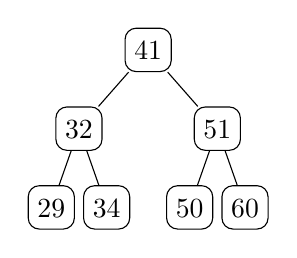
\begin{tikzpicture}[node distance = 2cm, auto, level distance=10mm, text depth=.1em, text height=.8em, level 1/.style={sibling distance=5em}, level 2/.style={sibling distance=2em},   baseline=(current bounding box.center)]
  \node[rectangle, draw, rounded corners] {41}
    child {node[rectangle, draw, rounded corners] {32}
      child {node[rectangle, draw, rounded corners] {29}}
      child {node[rectangle, draw, rounded corners] {34}}
    }
    child {node[rectangle, draw, rounded corners] {51}
      child {node[rectangle, draw, rounded corners] {50}}
      child {node[rectangle, draw, rounded corners] {60}}
    };
\end{tikzpicture}fuses to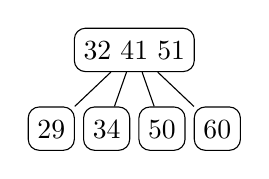
\begin{tikzpicture}[node distance = 2cm, auto, level distance=10mm, text depth=.1em, text height=.8em, level 1/.style={sibling distance=2em},   baseline=(current bounding box.center)]
  \node[rectangle, draw, rounded corners] {32 41 51}
    child {node[rectangle, draw, rounded corners] {29}}
    child {node[rectangle, draw, rounded corners] {34}}
    child {node[rectangle, draw, rounded corners] {50}}
    child {node[rectangle, draw, rounded corners] {60}};
\end{tikzpicture}\\

\definition{Transfer a $2\ Node$ and a $3\ Node$}
If a $2\ node$ is a sibling with a $3\ node$ we can transfer between the two.\
Let $n_2$ be a $2\ node$ and $n_3$ be a $3\ node$ which are siblings and $p$ be their parent.\\
We can transfer between $n_2$ \& $n_3$
\begin{enumerate}
  \item Identify the key of $p$ which forms a boundary between $n_2$ and $n_3$.
  \item Move this key to $n_2$, ensuring numerical order is maintained.
  \item Move the key of $n_3$ which is closest in value to the keys of $n_2$ to $p$, ensuring order is kept.
  \item Move the sub-tree of $n_3$ which is closest to $n_2$ to $n_2$, ensuring numerical order is maintained.
\end{enumerate}

\example{Transfer a $2\ Node$ and a $3\ Node$}
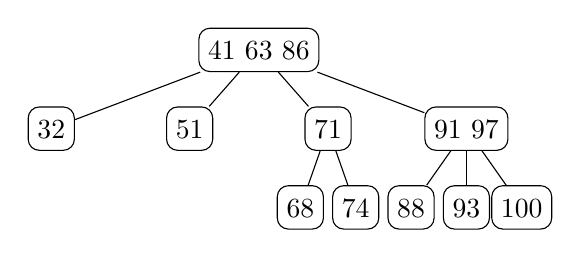
\begin{tikzpicture}[node distance = 2cm, auto, level distance=10mm, text depth=.1em, text height=.8em, level 1/.style={sibling distance=5em}, level 2/.style={sibling distance=2em},   baseline=(current bounding box.center)]
  \node[rectangle, draw, rounded corners] {41 63 86}
    child {node[rectangle, draw, rounded corners] {32}}
    child {node[rectangle, draw, rounded corners] {51}}
    child {node[rectangle, draw, rounded corners] {71}
      child {node[rectangle, draw, rounded corners] {68}}
      child {node[rectangle, draw, rounded corners] {74}}
    }
    child {node[rectangle, draw, rounded corners] {91 97}
      child {node[rectangle, draw, rounded corners] {88}}
      child {node[rectangle, draw, rounded corners] {93}}
      child {node[rectangle, draw, rounded corners] {100}}
    };
\end{tikzpicture}
transfers to
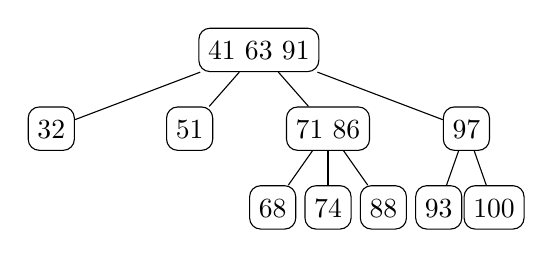
\begin{tikzpicture}[node distance = 2cm, auto, level distance=10mm, text depth=.1em, text height=.8em, level 1/.style={sibling distance=5em}, level 2/.style={sibling distance=2em},   baseline=(current bounding box.center)]
  \node[rectangle, draw, rounded corners] {41 63 91}
    child {node[rectangle, draw, rounded corners] {32}}
    child {node[rectangle, draw, rounded corners] {51}}
    child {node[rectangle, draw, rounded corners] {71 86}
      child {node[rectangle, draw, rounded corners] {68}}
      child {node[rectangle, draw, rounded corners] {74}}
      child {node[rectangle, draw, rounded corners] {88}}
    }
    child {node[rectangle, draw, rounded corners] {97}
      child {node[rectangle, draw, rounded corners] {93}}
      child {node[rectangle, draw, rounded corners] {100}}
    };
\end{tikzpicture}\\\\

\remark{Implementing 2-3-4 Tree}
Since it is complicated to implement \textit{2-3-4 Tree}s in code, coders often use \textit{Red-Black Tree}s instead.

\subsection{Skip Lists}

\definition{Multi-Level Linked Lists}
A \textit{Multi-Level Linked List} is a linked list which has several linked list above it.\\
Each of these linked lists is called a layer.\\
Each layers contains a subset of the elements of the list below it.\\
All layers contain the first and last elements of the linked list.\\
Each element links to its equivalent element in the list below.\\

\example{Multi-Level Linked List}
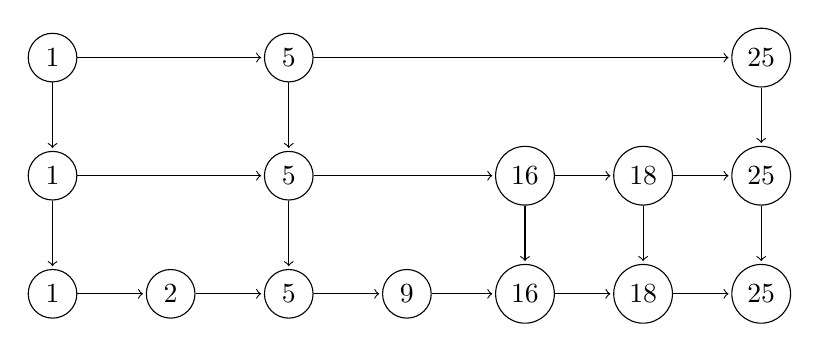
\begin{tikzpicture}[shorten >=1pt,node distance=1.5cm,on grid,auto]
   \node[circle, draw] (1_0) {1};
   \node[circle, draw] (2_0)  [right=of 1_0]  {2};
   \node[circle, draw] (5_0)  [right=of 2_0]  {5};
   \node[circle, draw] (9_0)  [right=of 5_0]  {9};
   \node[circle, draw] (16_0) [right=of 9_0]  {16};
   \node[circle, draw] (18_0) [right=of 16_0] {18};
   \node[circle, draw] (25_0) [right=of 18_0] {25};

   \node[circle, draw] (1_1)  [above=of 1_0]  {1};
   \node[circle, draw] (5_1)  [above=of 5_0]  {5};
   \node[circle, draw] (16_1) [above=of 16_0] {16};
   \node[circle, draw] (18_1) [above=of 18_0] {18};
   \node[circle, draw] (25_1) [above=of 25_0] {25};

   \node[circle, draw] (1_2)  [above=of 1_1]  {1};
   \node[circle, draw] (5_2)  [above=of 5_1]  {5};
   \node[circle, draw] (25_2) [above=of 25_1] {25};
    \path[->]
    (1_0)  edge (2_0)
    (2_0)  edge (5_0)
    (5_0)  edge (9_0)
    (9_0)  edge (16_0)
    (16_0) edge (18_0)
    (18_0) edge (25_0)
    (1_1)  edge (5_1)
           edge (1_0)
    (5_1)  edge (16_1)
           edge (5_0)
    (16_1) edge (18_1)
           edge (16_0)
    (18_1) edge (25_1)
           edge (18_0)
    (25_1) edge (25_0)
    (1_2)  edge (1_1)
           edge (5_2)
    (5_2)  edge (5_1)
           edge (25_2)
    (25_2) edge (25_1);
\end{tikzpicture}\\

\proposition{FIND(k) - Multi-Level Linked List}
Let $k$ be the key we are trying to find.
\begin{enumerate}[label=\roman*)]
  \item Start at first element of top level.
  \item Move right along level until you find key $k'>k$.
  \item Move down a level at the key before $k'$.
  \item Repeat ii) \& iii) until reach you kind $k$ and are in bottom level.
\end{enumerate}

\remark{Complexity of FIND(k) - Two-Level Linked List}
Let $m$ be the number of keys in the top row \& $n$ be the number of elements in the bottom row.\\
If the $m$ elements are evenly distributed $FIND(k)\in O(m+\frac{n}{m})$.\\
By setting $m=\sqrt{n}$ we get $FIND(k)\in O(m+\frac{n}{m})=O(\sqrt{n})$.\\

\definition{Skip List}
A \textit{Skip List} is a multi-level linked list which is constructed in a specific way.\\
The construction algorithm is a \textit{randomised algorithm}.
\begin{enumerate}[label=\roman*)]
  \item Create linked list of all elements and place as bottom level.
  \item Add level above containing just the first and last element.
  \item For each of the other elements randomly toss a coin:
  \begin{enumerate}
    \item HEADS - Add element to new layer.
    \item TAILS - Don't add element to new layer.
  \end{enumerate}
  \item Repeat ii) \& iii) until you produce a layer containing just the first and last elements.
\end{enumerate}

\example{Constructing Skip List}
Consider the following linked list and coin flips\\
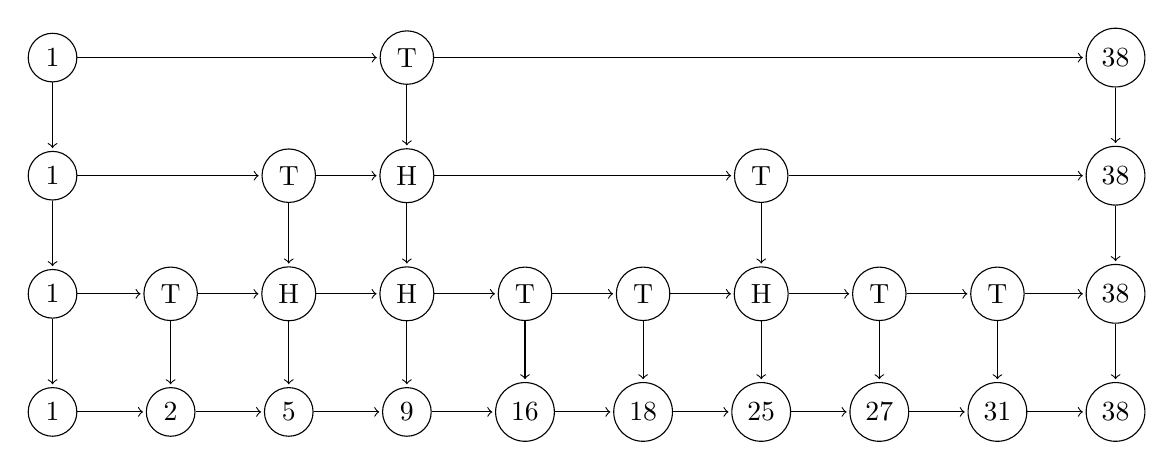
\begin{tikzpicture}[shorten >=1pt,node distance=1.5cm,on grid,auto]
   \node[circle, draw] (1_0) {1};
   \node[circle, draw] (2_0)  [right=of 1_0]  {2};
   \node[circle, draw] (5_0)  [right=of 2_0]  {5};
   \node[circle, draw] (9_0)  [right=of 5_0]  {9};
   \node[circle, draw] (16_0) [right=of 9_0]  {16};
   \node[circle, draw] (18_0) [right=of 16_0] {18};
   \node[circle, draw] (25_0) [right=of 18_0] {25};
   \node[circle, draw] (27_0) [right=of 25_0] {27};
   \node[circle, draw] (31_0) [right=of 27_0] {31};
   \node[circle, draw] (38_0) [right=of 31_0] {38};

   \node[circle, draw] (1_1)  [above=of 1_0]  {1};
   \node[circle, draw] (2_1)  [above=of 2_0]  {T};
   \node[circle, draw] (5_1)  [above=of 5_0]  {H};
   \node[circle, draw] (9_1)  [above=of 9_0]  {H};
   \node[circle, draw] (16_1) [above=of 16_0] {T};
   \node[circle, draw] (18_1) [above=of 18_0] {T};
   \node[circle, draw] (25_1) [above=of 25_0] {H};
   \node[circle, draw] (27_1) [above=of 27_0] {T};
   \node[circle, draw] (31_1) [above=of 31_0] {T};
   \node[circle, draw] (38_1) [above=of 38_0] {38};

   \node[circle, draw] (1_2)  [above=of 1_1]  {1};
   \node[circle, draw] (5_2)  [above=of 5_1]  {T};
   \node[circle, draw] (9_2)  [above=of 9_1]  {H};
   \node[circle, draw] (25_2) [above=of 25_1] {T};
   \node[circle, draw] (38_2) [above=of 38_1] {38};

   \node[circle, draw] (1_3)  [above=of 1_2]  {1};
   \node[circle, draw] (9_3)  [above=of 9_2]  {T};
   \node[circle, draw] (38_3) [above=of 38_2] {38};

    \path[->]
    (1_0)  edge (2_0)
    (2_0)  edge (5_0)
    (5_0)  edge (9_0)
    (9_0)  edge (16_0)
    (16_0) edge (18_0)
    (18_0) edge (25_0)
    (25_0) edge (27_0)
    (27_0) edge (31_0)
    (31_0) edge (38_0)

    (1_1)  edge (1_0)
    (2_1)  edge (2_0)
    (5_1)  edge (5_0)
    (9_1)  edge (9_0)
    (16_1) edge (16_0)
    (18_1) edge (18_0)
    (25_1) edge (25_0)
    (27_1) edge (27_0)
    (31_1) edge (31_0)
    (38_1) edge (38_0)

    (1_1)  edge (2_1)
    (2_1)  edge (5_1)
    (5_1)  edge (9_1)
    (9_1)  edge (16_1)
    (16_1) edge (18_1)
    (18_1) edge (25_1)
    (25_1) edge (27_1)
    (27_1) edge (31_1)
    (31_1) edge (38_1)

    (1_2)  edge (1_1)
    (5_2)  edge (5_1)
    (9_2)  edge (9_1)
    (25_2) edge (25_1)
    (38_2) edge (38_1)

    (1_2)  edge (5_2)
    (5_2)  edge (9_2)
    (9_2)  edge (25_2)
    (25_2) edge (38_2)

    (1_3)  edge (9_3)
    (9_3)  edge (38_3)

    (1_3)  edge (1_2)
    (9_3)  edge (9_2)
    (38_3) edge (38_2);
\end{tikzpicture}\\
Which produces the following skip list\\
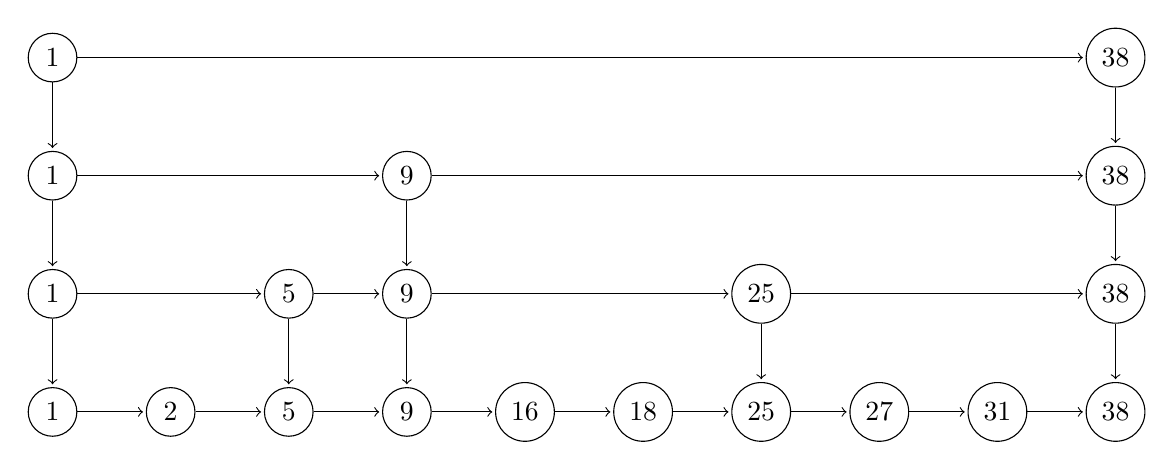
\begin{tikzpicture}[shorten >=1pt,node distance=1.5cm,on grid,auto]
   \node[circle, draw] (1_0) {1};
   \node[circle, draw] (2_0)  [right=of 1_0]  {2};
   \node[circle, draw] (5_0)  [right=of 2_0]  {5};
   \node[circle, draw] (9_0)  [right=of 5_0]  {9};
   \node[circle, draw] (16_0) [right=of 9_0]  {16};
   \node[circle, draw] (18_0) [right=of 16_0] {18};
   \node[circle, draw] (25_0) [right=of 18_0] {25};
   \node[circle, draw] (27_0) [right=of 25_0] {27};
   \node[circle, draw] (31_0) [right=of 27_0] {31};
   \node[circle, draw] (38_0) [right=of 31_0] {38};

   \node[circle, draw] (1_1)  [above=of 1_0]  {1};
   \node[circle, draw] (5_1)  [above=of 5_0]  {5};
   \node[circle, draw] (9_1)  [above=of 9_0]  {9};
   \node[circle, draw] (25_1) [above=of 25_0] {25};
   \node[circle, draw] (38_1) [above=of 38_0] {38};

   \node[circle, draw] (1_2)  [above=of 1_1]  {1};
   \node[circle, draw] (9_2)  [above=of 9_1]  {9};
   \node[circle, draw] (38_2) [above=of 38_1] {38};

   \node[circle, draw] (1_3)  [above=of 1_2]  {1};
   \node[circle, draw] (38_3) [above=of 38_2] {38};

    \path[->]
    (1_0)  edge (2_0)
    (2_0)  edge (5_0)
    (5_0)  edge (9_0)
    (9_0)  edge (16_0)
    (16_0) edge (18_0)
    (18_0) edge (25_0)
    (25_0) edge (27_0)
    (27_0) edge (31_0)
    (31_0) edge (38_0)

    (1_1)  edge (1_0)
    (5_1)  edge (5_0)
    (9_1)  edge (9_0)
    (25_1) edge (25_0)
    (38_1) edge (38_0)

    (1_1)  edge (5_1)
    (5_1)  edge (9_1)
    (9_1)  edge (25_1)
    (25_1) edge (38_1)

    (1_2)  edge (1_1)
    (9_2)  edge (9_1)
    (38_2) edge (38_1)

    (1_2)  edge (9_2)
    (9_2)  edge (38_2)

    (1_3)  edge (38_3)

    (1_3)  edge (1_2)
    (38_3) edge (38_2);
\end{tikzpicture}\\

\proposition{Number of Levels in Skip List}
An empty skip list contains only one level, and the only way to increase the number of levels is during $INSERT$.\\
The probability of increasing the number of levels if $\frac{1}{2}$ and the number of levels only every increases by $1$.\\
Thus the probability of $INSERT$ adding $n$ levels is $\frac{1}{2^n}$ and this tends to $0$ very quickly.\\
The probability of $INSERT$ adding $2\log_2n$ levels is $\frac{1}{2^{2\log_2n}}=\frac{1}{n^2}$.\\
Consider the \textit{Union Bound Theorem}.\\
Let $E_j$ be the event where the $j^{th}\ INSERT$ puts its element in more than $2\log_2n$ levels.\\
Then the probability that $E_1,\dots,E_j$ all occur at level one is at most $\sum_{i=1}^j\frac{1}{n^2}=\frac{1}{n}$.\\
Thus it is very unlikely for a skip list to have $2\log_2n$ levels and the number of levels is $O(\log_2n)$.\\

\remark{Constructing Skip List in Practice}
In practice you may want to consider setting a constant $x$ so if a generated level has $<x$ elements you stop randomising.\\
This prevents having multiple duplicate layers higher up the skip list since duplicates become more likely with less elements and don't improve traversing at all.\\
Alternatively you could randomise the whole process and then evaluate the resulting skip list, removing duplicate layers.

\subsection{Flow Networks}

\definition{Flow Network}
A \textit{Flow Network} is a directed graph where every edge has a non-negative \textit{capacity}.\\ Exactly one node within a \textit{Flow Network}is referred to as the \textit{Source} \& exactly one node as the \textit{Sink}.\\
The aim of a \textit{Flow Network} is to move the maximum amount of material from the source to the sink.\\

\definition{Capacity}
\textit{Capacity} is a map from an edge to a non-negative real value.\\
When an edge has zero \textit{Capacity} it is not shown.\\
The \textit{Capacity} of an edge is the maximum amount of flow along that edge.\\
\nb $c:V\times V\to\real^{\geq0}$.\\

\newpage
\definition{Flow}
The \textit{Flow} in the network $G$ is a function $f:V\times V\to\real^{\geq0}$.\\
The \textit{Flow} function must satisfy the following conditions
\begin{enumerate}
	\item $\forall\ u,v\in V\ 0\leq f(u,v)\leq c(u,v)$.\\
	The flow along an edge is non-negative \& cannot exceed the capacity of that edge;
	\item And, $\forall\ u\in V\setminus\{s,t\}\ \sum_{v\in V}f(u,v)=\sum_{v\in V}f(v,u)$.\\
	The flow into all nodes, except the source \& sink, must equal the flow out of the node.
\end{enumerate}
\nb The same network can have multiple flow functions.\\

\definition{Value}
The \textit{Value} of a flow $f$ is defined as
$$|f|:=\sum_{v\in V}f(v,t)-f(t,v)$$
\nb This is the total flow into the terminal, less the total flow out of it.\\

\example{Flow Network}
Here is an example of a \textit{Flow Network}.\\
The capacity \& flow are denoted as $f/c$.\\
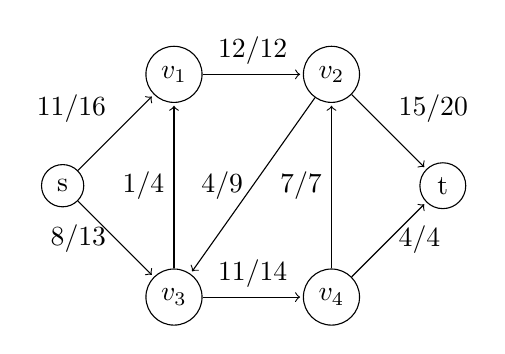
\begin{tikzpicture}[shorten >=1pt,node distance=2cm,on grid,auto]
   \node[circle, draw] (s)  {s};
   \node[circle, draw] (v1) [above right=of s]  {$v_1$};
   \node[circle, draw] (v2) [right=of v1]       {$v_2$};
   \node[circle, draw] (v3) [below right=of s]  {$v_3$};
   \node[circle, draw] (v4) [right=of v3]       {$v_4$};
   \node[circle, draw] (t)  [above right=of v4] {t};
   
   \path[->]
    (s)  edge node        {$11/16$} (v1)
         edge node[left]  {$8/13$}  (v3)
    (v1) edge node        {$12/12$} (v2)
    (v2) edge node        {$15/20$} (t)
         edge node[left]  {$4/9$}   (v3)
    (v3) edge node        {$1/4$}   (v1)
         edge node        {$11/14$} (v4)
    (v4) edge node        {$7/7$}   (v2)
         edge node[right] {$4/4$}   (t);
\end{tikzpicture}\\
\nb Here $|f|=f(v_2,t)+f(v_4,t)-0=15+4=19$.\\

\definition{Antiparallel Edges}
An \textit{Antiparrallel} edge is a pair of vertices $u\ \&\ v$ where $f(u,v)>0$ \& $f(v,u)>0$.\\
\nb Each direction can have a different flow or capacity.\\

\proposition{Removing Antiparallel Edges}
We can remove \textit{Antiparallel Edges} from a flow network by adding a new node and having one of the directions pass through that node, keeping the same capacity \& flow.\\

\newpage
\example{Removing Antiparallel Edges}
Here we remove the \textit{Anti-Parallel} edge between $v_3$ \& $v_4$.\\
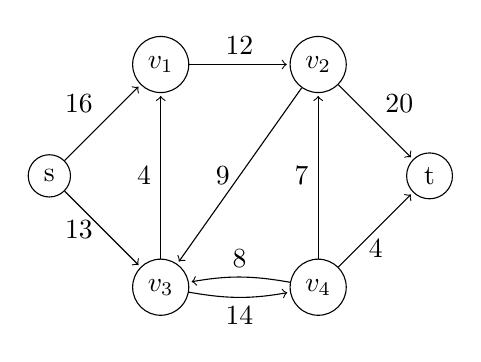
\begin{tikzpicture}[shorten >=1pt,node distance=2cm,on grid,auto, baseline=(current bounding box.center)]
   \node[circle, draw] (s)  {s};
   \node[circle, draw] (v1) [above right=of s]  {$v_1$};
   \node[circle, draw] (v2) [right=of v1]       {$v_2$};
   \node[circle, draw] (v3) [below right=of s]  {$v_3$};
   \node[circle, draw] (v4) [right=of v3]       {$v_4$};
   \node[circle, draw] (t)  [above right=of v4] {t};
   
   \path[->]
    (s)  edge 				 node 		 {$16$} (v1)
         edge 				 node[left]  {$13$} (v3)
    (v1) edge 				 node 		 {$12$} (v2)
    (v2) edge 				 node 		 {$20$} (t)
         edge 				 node[left]  {$9$}  (v3)
    (v3) edge                node 		 {$4$}  (v1)
         edge[bend right=10] node[below] {$14$} (v4)
    (v4) edge 				 node 		 {$7$}  (v2)
         edge 				 node[below] {$4$}  (t)
         edge[bend right=10] node[above] {$8$}  (v3);
\end{tikzpicture}
becomes
\begin{tikzpicture}[shorten >=1pt,node distance=2cm,on grid,auto, baseline=(current bounding box.center)]
   \node[circle, draw] (s)  {s};
   \node[circle, draw] (v1) [above right=of s]  {$v_1$};
   \node[circle, draw] (v2) [above left=of t]   {$v_2$};
   \node[circle, draw] (v3) [below right=of s]  {$v_3$};
   \node[circle, draw] (v4) [below left=of t]   {$v_4$};
   \node[circle, draw] (v5) [below =of v3]      {$v_5$};
   \node[circle, draw] (t)  [above right=of v4] {t};
   
   \path[->]
    (s)  edge node 		  {$16$} (v1)
         edge node[left] {$13$} (v3)
    (v1) edge node 		  {$12$} (v2)
    (v2) edge node 		  {$20$} (t)
         edge node[left] {$9$} (v3)
    (v3) edge node 		  {$4$} (v1)
         edge node[below] {$14$} (v4)
    (v4) edge node        {$7$} (v2)
         edge node[below] {$4$} (t)
         edge node[right] {$8$} (v5)
    (v5) edge node[left] {$8$} (v3);
\end{tikzpicture}

\proposition{Multiple Sources\textbackslash Sinks}
We can transform a flow network with multiples sources or sinks to only have one.\\

\example{Multiple Sources\textbackslash Sinks}
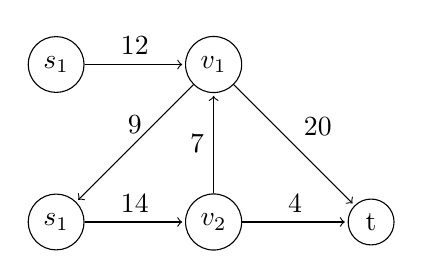
\begin{tikzpicture}[shorten >=1pt,node distance=2cm,on grid,auto, baseline=(current bounding box.center)]
   \node[circle, draw] (v1) {$s_1$};
   \node[circle, draw] (v2) [right=of v1]  {$v_1$};
   \node[circle, draw] (v3) [below =of v1] {$s_1$};
   \node[circle, draw] (v4) [right=of v3]  {$v_2$};
   \node[circle, draw] (t)  [right=of v4]  {t};
   
   \path[->]
    (v1) edge node 		  {$12$} (v2)
    (v2) edge node 		  {$20$} (t)
         edge node[above] {$9$}  (v3)
    (v3) edge node 		  {$14$} (v4)
    (v4) edge node 		  {$7$}  (v2)
         edge node[above] {$4$}  (t);
\end{tikzpicture}
becomes
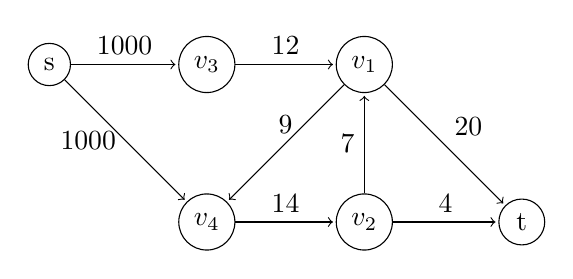
\begin{tikzpicture}[shorten >=1pt,node distance=2cm,on grid,auto, baseline=(current bounding box.center)]
   \node[circle, draw] (s)  {s};
   \node[circle, draw] (v1) [right=of s]  {$v_3$};
   \node[circle, draw] (v2) [right=of v1] {$v_1$};
   \node[circle, draw] (v3) [below=of v1] {$v_4$};
   \node[circle, draw] (v4) [right=of v3] {$v_2$};
   \node[circle, draw] (t)  [right=of v4] {t};
   
   \path[->]
    (s)  edge node 		  {$1000$} (v1)
         edge node[left]  {$1000$} (v3)
    (v1) edge node 		  {$12$}   (v2)
    (v2) edge node 		  {$20$}   (t)
         edge node[above] {$9$}    (v3)
    (v3) edge node 		  {$14$}   (v4)
    (v4) edge node 		  {$7$}    (v2)
         edge node[above] {$4$}    (t);
\end{tikzpicture}\\

\definition{Residual Network}
Consider being given a flow network $G$ \& a flow $f$.\\
The \textit{Residual Network} for this $G$ \& $f$ is $G_f$ where
$$E_f=\{(u,v)\in V\times V:c_f(u,b)\geq 0\}$$
where
\[
c_f(u,v)=\begin{cases}
c(u,v)-f(u,v),& (u,v)\in E\\
f(v,u),& (v,u)\in E\\
0,& otherwise
\end{cases}
\]

\example{Residual Network}
Flow Network\quad\quad\quad\quad\quad\quad\quad\quad\quad\quad\quad\quad\quad  Residual Network\\
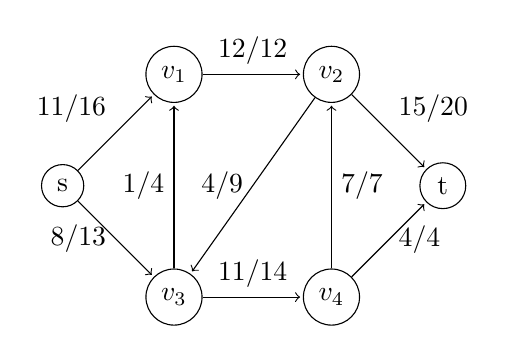
\begin{tikzpicture}[shorten >=1pt,node distance=2cm,on grid,auto, baseline=(current bounding box.center)]
   \node[circle, draw] (s) {s};
   \node[circle, draw] (v1)  [above right=of s]  {$v_1$};
   \node[circle, draw] (v2)  [right=of v1]  {$v_2$};
   \node[circle, draw] (v3)  [below right=of s]  {$v_3$};
   \node[circle, draw] (v4) [right=of v3]  {$v_4$};
   \node[circle, draw] (t) [above right=of v4] {t};
   
   \path[->]
    (s)  edge node 		  {$11/16$} (v1)
         edge node[left]  {$8/13$}  (v3)
    (v1) edge node 		  {$12/12$} (v2)
    (v2) edge node 		  {$15/20$} (t)
         edge node[left]  {$4/9$}   (v3)
    (v3) edge node 		  {$1/4$}   (v1)
         edge node 		  {$11/14$} (v4)
    (v4) edge node[right] {$7/7$}   (v2)
         edge node[right] {$4/4$}   (t);
\end{tikzpicture}
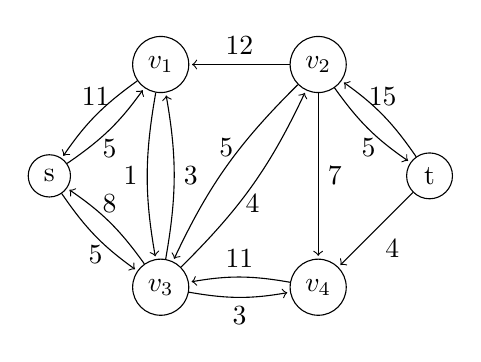
\begin{tikzpicture}[shorten >=1pt,node distance=2cm,on grid,auto, baseline=(current bounding box.center)]
   \node[circle, draw] (s) {s};
   \node[circle, draw] (v1)  [above right=of s]  {$v_1$};
   \node[circle, draw] (v2)  [right=of v1]  {$v_2$};
   \node[circle, draw] (v3)  [below right=of s]  {$v_3$};
   \node[circle, draw] (v4) [right=of v3]  {$v_4$};
   \node[circle, draw] (t) [above right=of v4] {t};
   
   \path[->]
   (s)  edge[bend right=10] node[below] {5}  (v1)
        edge[bend right=10] node[below] {5}  (v3)
   (v1) edge[bend right=10] node[above] {11} (s)
        edge[bend right=10] node[left]  {1}  (v3)
   (v2) edge                node[above] {12} (v1)
        edge[bend right=10] node[above] {5}  (v3)
        edge                node        {7}  (v4)
        edge[bend right=10] node[below] {5}  (t)
   (v3) edge[bend right=10] node[above] {8}  (s)
        edge[bend right=10] node[right] {3}  (v1)
        edge[bend right=10] node[below] {4}  (v2)
        edge[bend right=10] node[below] {3}  (v4)
   (v4) edge[bend right=10] node[above] {11} (v3)
   (t)  edge[bend right=10] node[above] {15} (v2)
        edge                node        {4}  (v4);
\end{tikzpicture}

\definition{Augmenting Path}
An \textit{Augmenting Path} is a simple path\footnote{See \textbf{Data Structures:Definition 1.2}} from source to sink in the residual network.\\

\definition{Residual Capacity}
The \textit{Residual Capacity} of an augmenting path $p$ is given by $c_f(p)=min\{c_f(u,v):(u,v)\in p\}$.\\

\definition{Augmentation of Flow}
Let $f$ be a flow in a flow network $G$ \& $f'$ be a flow in the residual network $G_f$.\\
The \textit{Augmentation} of $f$ by $f'$ is a function $f\uparrow f':V\times V\to\real$.\\
This function is defined such that $f\uparrow f'(u,v)=f(u,v)+f'(u,v)-f'(v,u)$.\\

\definition{Cut}
A \textit{Cut} of a flow network is a partition of the vertex set into two sets, $S$ \& $T$, such that $$s\in S,\ t\in T,\ S\cap T=\emptyset$$

\definition{Net Flow of a Cut}
Let $f$ be a flow.\\
The \textit{Net Flow} across a cut with sets $S$ \& $T$ is defined as
$$f(S,T):=\sum_{u\in S}\sum_{v\in T}f(u,v)-\sum_{u\in S}\sum_{v\in T}f(v,u)$$

\definition{Capacity of a Cut}
The \textit{Capacity} of a cut with sets $S$ \& $T$ is defined as
$$c(S,T):=\sum_{u\in S}\sum_{v\in T}c(u,v)$$

\definition{Minimum Cut}
A \textit{Minimum Cut} is a cut whose capacity is the minimum of all possible cuts a given flow network.\\
\nb There can be multiple such cuts.\\

\theorem{Net Flow of a Cut}
Let $f$ be a flow with value $|f|$ in a flow network.\\
Let $(S,T)$ be any cut of the same flow network.\\
Then $f(S,T)=|f|$.\\

\proof{Theorem 8.1}
\textit{This is a mathematical proof for \textbf{Theorem 8.1}}.
\[\begin{array}{rcl}
|f|&=&\sum_{v\in V}f(s,v)-\sum_{v\in V}f(v,s)\\
&=&\sum_{v\in V}f(s,v)-\sum_{v\in V}f(v,s)\\
&+&\sum_{u\in S\setminus\{s\}}\sum_{v\in V}[f(u,v)-f(v,u)]\\
&=&\sum_{v\in V}[f(s,v)+\sum_{u\in S\setminus\{s\}}f(u,v)]\\
&-&\sum_{v\in V}[f(v,s)+\sum_{u\in S\setminus\{s\}}f(v,u)]\\
&=&\sum_{v\in V}[\sum_{u\in S}f(u,v)-\sum_{u\in S}f(v,u)]\\
&=&\sum_{v\in V}[\sum_{u\in S}f(u,v)-\sum_{u\in S}f(v,u)]\\
&+&\sum_{v\in T}[\sum_{u\in S}f(u,v)-\sum_{u\in S}f(v,u)]\\
&=&\sum_{v\in S}\sum_{u\in S}f(u,v)-\sum_{v\in S}\sum_{u\in S}f(v,u)\\
&+&\sum_{v\in T}\sum_{u\in S}f(u,v)-\sum_{v\in T}\sum_{u\in S}f(v,u)\\
&=&\sum_{v\in T}\sum_{u\in S}f(u,v)-\sum_{v\in T}\sum_{u\in S}f(v,u)\\
&=&\sum_{u\in S}\sum_{v\in T}f(u,v)-\sum_{u\in S}\sum_{v\in T}f(v,u)\\
&=&f(S,T)
\end{array}\]
\nb This is non-examinable.\\

\theorem{Max-Flow Min-Cut-Theorem}
The maximum flow value of a flow network is equal to its the minimum cut capacity.\\

\proof{Theorem 8.2}
Suppose $f$ is a maximum flow in a flow network $G$.\\
By \textbf{Theorem 8.1}, $|f|=f(S,T)\ \forall$ cuts $(S,T)\in G$.\\
Then $|f|\leq c(S,T)\ \forall$ cuts $(S,T)\in G$.\\
$G_f$ cannot have any paths from $s\to t$, as if there was one you could augment $f$ along the path to create a flow with greater value.\\
Let $S$ be the set of vertices $u$ for which there is a path $s\to u$ in $G_f$.\\
Let $T=V-S$.\\
Suppose $u\in S,\ v\in T$.\\
Then $(u,v)$ cannot be in $G_f$, otherwise $v$ would be in $S$.\\
If $(u,v)\in G$ then $f(u,v)=c(u,v)$.\\
If $(v,u)\in G$ then $f(v,u)=0$.\\
\[\begin{array}{rcccl}
|f|&=&f(S,T)&=&\sum_{u\in S}\sum_{v\in T}f(u,v)-\sum_{u\in S}\sum_{v\in T}f(v,u)\\
&&&=&\sum_{u\in S}\sum_{v\in T}c(u,v)\\
&&&=&c(S,T)
\end{array}\]
We know that $|f|\leq c(S',T')\ \forall$ cuts $(S',T')\in G$.\\
Thus $c(S,T)$ must be the minimum cut capacity.\\ 

\remark{Modelling with Flow Networks}
\textit{Flow Networks} are used to model road networks, computer networks, sewers etc.\\

\proposition{Max Flow-Min Cut Theorem for Image Segmentation}
The \textit{Max Flow-Min Cut Theorem} can be used for image segmentation.\\
The aim of image segmentation is to split an image into its foreground \& background.\\
Represent the pixels as nodes, creating edges to neighbouring pixels and setting the weight of each edge to be the difference in colour between the pixels.\\
Adding two new nodes, one for source \& one for sink, which connect to all pixel nodes we can now perform \textit{Max Flow-Min Cut} to create a cut.\\
\nb This is non-examinable.

\subsection{Miscellaneous}

\definition{Finite State Machine}
A \textit{Finite State Machine} is a computation model used to simulate sequential logic.\\
\textit{Finite State Machine}s must have the follow features
\begin{enumerate}[label=\roman*)]
  \item A finite set of states $Q$;
  \item An initial state $q_0\in Q$;
  \item A set of accepting states $A\subset Q$;
  \item An input alphabet $\Sigma$; And,
  \item A transition function $\delta:Q\times\Sigma \to Q$.
\end{enumerate}

\remark{Applications of Finite State Machines}
Finite state machines can be used to detect regular expression patterns\footnote{See \textbf{Algorithms:Proposition 4.2}}.\\
\nb A coded example of this can be seen in {\ttfamily{programs/FiniteStateMachine.java}} and {\ttfamily{programs/PatternMatcher.java:finiteStateMachine}}.\\

\definition{Prefix Table}
The \textit{Prefix Table}, $\pi$, for a string $S$ is the integer array where $\pi[i]$ gives the length of the longest substring of $S[0,\dots,i-1]$ which is both a suffix and a prefix to $S[0,\dots,i]$.\\
Note that this substring cannot be equal to $S[0,\dots,i]$.\\

\proposition{Pseudocode for Constructing a Prefix Table}
A \textit{Prefix Table}, for the string $S$, can be constructed using the following pseudocode\footnote{See \ttfamily{programs\textbackslash PrefixTable.java}}
\begin{code}
PREFIX(S)
$\pi$=[]
for (i=1; i<S.length; i++):
  c=0
  $\pi$[i]=0
  for (j=1; j<i; j++:
    prefix=S[0,j]
    suffix=S[i-j,i];
    if (prefix==suffix):
      $\pi$[i]=c
return $\pi$
\end{code}
\nb This algorithm assumes strings are zero-indexed.\\

\example{Constructing Prefix Table}
Here we shall construct a prefix table for the string \textit{``aaabbb"}.\\
\\\underline{Substring} - \textit{``a"}\\
Set $\pi[0]=0$.\\
Prefix cannot be whole string. Stop.\\
\\\underline{Substring} - \textit{``aa"}\\
Set $\pi[1]=0$.\\
prefix=\textit{``a"}==\textit{``a"}=suffix. Continue.\\
Set $\pi[1]=1$.\\
Prefix cannot be the whole string. Stop\\
\\\underline{Substring} - \textit{``aaa"}\\
Set $\pi[2]=0$.\\
prefix=\textit{``a"}==\textit{``a"}=suffix. Continue.\\
Set $\pi[2]=1$.\\
prefix=\textit{``aa"}==\textit{``aa"}=suffix. Continue.\\
Set $\pi[2]=1$.\\
Prefix cannot be the whole string. Stop.\\
\\\underline{Substring} - \textit{``aaab"}\\
Set $\pi[3]=0$.\\
prefix=\textit{``a"}$\neq$\textit{``b"}=suffix. Stop.\\
\\\underline{Substring} - \textit{``aaabb"}\\
Set $\pi[4]=0$.\\
prefix=\textit{``a"}$\neq$\textit{``b"}=suffix. Stop.\\
\\\underline{Substring} - \textit{``aaabbb"}\\
Set $\pi[5]=0$.\\
prefix=\textit{``a"}$\neq$\textit{``b"}=suffix. Stop.\\
\\The Prefix Table for \textit{``aaabbb"} is $\pi=[0,1,2,0,0,0]$.\\

\definition{Bad Match Table}
A \textit{Bad Match Table} for a string is a map from each character in the string's alphabet to an integer.\\
This integer is the number of places you should shift the pattern along if the associated character is the character from the target text which causes a mismatch.\\

\proposition{Pseudocode for Constructing a Bad Match Table}
A \textit{Bad Match Table} for the string $S$ can be constructed using the following pseudocode\footnote{See \ttfamily{programs\textbackslash BadMatchTable.java}}
\begin{code}
BadMatchTable(S)
table=[]
table['*']=S.length
for (i=0; i<S.length; i++):
  char=S[i]
  table[char]=i
return table
\end{code}

\example{Constructing Bad Match Table}
Here we shall construct a bad match table for the string \textit{``tooth"}.\\

Set $table['*']=5$.\\
Set $table['t']=0$.\\
Set $table['o']=1$.\\
Set $table['o']=2$.\\
Set $table['t']=3$.\\
Set $table['h']=4$.\\
\\
The Bad Match Table for \textit{``tooth"} is $['t':3,\ 'o':2,\ 'h':4,\ '*':5]$.

\newpage
\section{Algorithms}

\subsection{Sorting}

\definition{Insertion Sort}
\textit{Insertion Sort} is an in-place sorting algorithm.\\
\textit{Insertion Sort} can be performed on the ordable array $A$ with the following pseudocode.\footnote{See \ttfamily{programs\textbackslash Sort.java}}
\begin{code}
INSERTION-SORT(A)
for (j=1; j<A.length; j++):
  key=A[j]
  i=j-1
  while (i>-1 && A[i]>key):
    A[i+1]=A[i]
    i--
  A[i+1] = key
return A
\end{code}

\theorem{Asymptotic Analysis of Insertion Sort}
The average case run-time complexity for insertion sort is $\in O(n^2)$.\\
The best case run-time complexity for insertion sort is $\in O(n)$.\\
The space complexity for insertion sort is $\in O(n)$.\\

\example{Insertion Sort}
Here we sort the list $[3,4,5,1,2]$.\\
$3$ is already sorted.\\
Sort $4$.\\
Compare $4$ \& $3$. $4>3$ Stop.\\
$[3,4,5,1,2]$.\\
Sort $5$.\\
Compare $5$ \& $4$. $5>4$ Stop.\\
$[3,4,5,1,2]$.\\
Sort $1$.\\
Compare $1$ \& $5$. $1<5$ Swap.\\
Compare $1$ \& $4$. $1<4$ Swap.\\
Compare $1$ \& $3$. $1<3$ Swap.\\
End of list. Stop.\\
$[1,3,4,5,2]$.\\
Sort $2$.\\
Compare $2$ \& $5$. $2<5$ Swap.\\
Compare $2$ \& $4$. $2<4$ Swap.\\
Compare $2$ \& $3$. $2<3$ Swap.\\
Compare $2$ \& $1$. $2>1$ Stop.\\
$[1,2,3,4,5]$.\\

\proof{Correctness of Insertion Sort}
Here we prove that \textit{Insertion Sort} is a loop invariant.\\
\textit{Initialisation}\\
Set $j=2$ then the array $A]1, \dots, j-1]$ has only one element, thus it is sorted.\\
\textit{Maintenance}\\
The \textit{for} loop moves $A[j-1], A[j-2], \dots$ to the right until it finds the position for $A[j]$ so $A[1, \dots, j]$ is sorted. Thus invariance holds.\\
\textit{Termination}\\
Since the loop has a predetermined termination value for $j$ then termination is quaranteed.\\
Thus invariance holds.\\
Since we have proved \textit{initialisation}, \textit{maintenance} \& \textit{termination} we have proved that insertion sort is a preserved invariant.\\

\definition{Merge Sort}
\textit{Merge Sort} is an in-place sorting algorithm.\\
\textit{Merge Sort} can be performed on the ordable array $A$ with the following pseudocode.\footnote{See \ttfamily{programs\textbackslash Sort.java}}
\begin{code}
MERGE-SORT(A,l,r)
n=A.length
if (n==1):
  return A
MERGE-SORT(A,l,n/2)
MERGE-SORT(A,n/2,r)
return MERGE(A,l,n/2,r)

MERGE(A,l,m,r)
L=A[l, m]
R=A[m, r]
i=0; j=0; k=0
while (i<m-l+1 && j<r-m):
  k++
  if (L[i]<=R[j]):
    A[k]=L[i]
    i++
  else:
  	A[k]=R[j]
  	j++
while (i<m-l+1):
  A[k]=L[i]
  i++; k++
while (j<r-m):
  A[k]=R[j]
  j++; k++
return A
\end{code}
\nb $l$ is the left bound \& $r$ is the right bound. Initially these are set so $l=0$ \& $r=A.length$.\\

\theorem{Asymptotic Analysis of Merge Sort}
The run-time complexity for merge sort is $\in O(n\log_2n)$.\\
The space complexity for insertion sort is $\in O(n)$.\\

\example{Merge Sort}
Here we sort the list $[3,4,5,1,2]$.\\
Split $[3,4,5,1,2]$ into $[3,4,5]$ \& $[1,2]$.\\
Split $[3,4,5]$ into $[3,4]$ \& $[5]$.\\
Split $[3,4]$ into $[3]$ \& $[4]$.\\
Merge $[3]$ \& $[4]$ into $[3,4]$.\\
Merge $[3,4]$ \& $[5]$ into $[3,4,5]$.\\
Split $[1,2]$ into $[1]$ \& $[2]$.\\
Merge $[1]$ \& $[2]$ into $[1,2]$.\\
Merge $[3,4,5]$ \& $[1,2]$ into $[1,2,3,4,5]$.\\

\proof{Run-Time Complexity for Merge Sort}
\textit{This is a proof by strong induction}.\\
\textit{Base Case}\\
$n=1\ a=T(1)$\\
\textit{Inductive Hypothesis}\\
The time complexity of merge sort for a list of $n$ objects is given by
$$T(m)=am+bm\log_2m\ \forall m<n,\ a,b\in\real$$
\textit{Inductive Step}
\[\begin{array}{rcl}
T(n) &=& 2T\left(\frac{n}{2}\right)+cn\\
\mathrm{By\ hypothesis}&=&2\left(a\frac{n}{2}+b.\frac{n}{2}.\log_2\left(\frac{n}{2}\right)\right)+cn\\
&=& an+bn\log_2n-bn+cn\\
\mathrm{For\ }b=c&=&an+bn.\log_2n
\end{array}\]
This is true $\forall\ n$ with $a=T(1)\ \&\ b=c$.\\\\
By the theorem of strong induction, $T(n)$ is the upper bounded for the worst case time for merge sort.
$$T(n)<(T(1)+c)n\log_2(n)\implies T(n)\in O(n\log_2(n))$$

\definition{Heap Sort}
\textit{Heap Sort} is an out-of-place sorting algorithm.\\
\textit{Heap Sort} can be performed on the ordable array $A$ with the following pseudocode.
\begin{code}
HEAP-SORT(A)
p=PRIORITY-QUEUE
B=[]
for i=0 to A.length:
  p.INSERT(A[i])
for i=0 to A.length:
  B[i]=p.EXTRACT-MIN()
return B
\end{code}

\example{Heap Sort}
Here we sort the list $[3,4,5,1,2]$ using \textit{Heap Sort}.\\
We shall implement the priority queue with a binary heap.\\
\\
Insert 3.\\\begin{tikzpicture}[node distance = 2cm, auto, level distance=10mm, text depth=.1em, text height=.8em, level 1/.style={sibling distance=2em},   baseline=(current bounding box.center)]
  \node {3};
\end{tikzpicture}\\
Insert 4.\\
\begin{tikzpicture}[node distance = 2cm, auto, level distance=10mm, text depth=.1em, text height=.8em, level 1/.style={sibling distance=2em},   baseline=(current bounding box.center)]
  \node {3}
    child {node {4}};
\end{tikzpicture}\\
Insert 5.\\
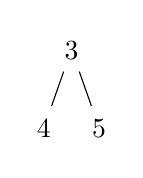
\begin{tikzpicture}[node distance = 2cm, auto, level distance=10mm, text depth=.1em, text height=.8em, level 1/.style={sibling distance=2em},   baseline=(current bounding box.center)]
  \node {3}
    child {node {4}}
    child {node {5}};
\end{tikzpicture}\\
\newpage
Insert 1.\\
\begin{tikzpicture}[node distance = 2cm, auto, level distance=10mm, text depth=.1em, text height=.8em, level 1/.style={sibling distance=2em},   baseline=(current bounding box.center)]
  \node {1}
    child {node {3}
      child {node {4} }
    }
    child {node {5}};
\end{tikzpicture}\\
Insert 2.\\
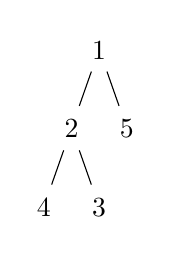
\begin{tikzpicture}[node distance = 2cm, auto, level distance=10mm, text depth=.1em, text height=.8em, level 1/.style={sibling distance=2em},   baseline=(current bounding box.center)]
  \node {1}
    child {node {2}
      child {node {4} }
      child {node {3} }
    }
    child {node {5}};
\end{tikzpicture}\\
Extract-min() = 1. $[1]$.\\
\begin{tikzpicture}[node distance = 2cm, auto, level distance=10mm, text depth=.1em, text height=.8em, level 1/.style={sibling distance=2em},   baseline=(current bounding box.center)]
  \node {2}
    child {node {3}
      child {node {4} }
    }
    child {node {5}};
\end{tikzpicture}\\
Extract-min() = 2. $[1,2]$.\\
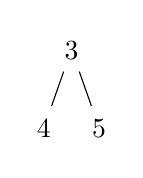
\begin{tikzpicture}[node distance = 2cm, auto, level distance=10mm, text depth=.1em, text height=.8em, level 1/.style={sibling distance=2em},   baseline=(current bounding box.center)]
  \node {3}
    child {node {4} }
    child {node {5}};
\end{tikzpicture}\\
Extract-min() = 3. $[1,2,3,]$.\\
\begin{tikzpicture}[node distance = 2cm, auto, level distance=10mm, text depth=.1em, text height=.8em, level 1/.style={sibling distance=2em},   baseline=(current bounding box.center)]
  \node {4}
    child {node {5}};
\end{tikzpicture}\\
Extract-min() = 4. $[1,2,3,4]$.\\
\begin{tikzpicture}[node distance = 2cm, auto, level distance=10mm, text depth=.1em, text height=.8em, level 1/.style={sibling distance=2em},   baseline=(current bounding box.center)]
  \node {5};
\end{tikzpicture}\\
Extract-min() = 5. $[1,2,3,4,5]$.\\
The priority queue is now empty so heap sort is complete.\\
$[1,2,3,4,5]$.\\

\theorem{Asymptotic Analysis on Heap Sort}
When \textit{Heap Sort} is performed using a binary heap, with the minimum-heap property, its run-time complexity is $\in O(n\log_2n)$.\\
The space complexity for heap sort is $\in O(n)$.

\subsection{Stable Matching}

\definition{Stable Match}
A matching is considered a \textit{stable match} if, either:
\begin{itemize}
\item[-] Both members prefer their partner over all others. Or,
\item[-] If one/both members prefer another partner, then this preferred partner prefers their current partner over the new suitor.
\end{itemize}
\nb These situations are the same.\\

\newpage
\definition{Stable Matching Problem}
Consider having two sets of people, $X$ \& $Y$.\\
Each person has a preference order for whom they wish to pair up with in the other group.\\
and you are matching one member of $X$ with one member of $Y$.\\
The \textit{Stable Matching Problem} is to find a group of pairings where every pair is a \textit{stable match}.\\

\definition{Feasible Pairing}
A pair $(x,y)$ is a \textit{Feasible Pairing} if there exists a stable matching of the sets $X$ \& $Y$ which includes $(x,y)$.\\

\theorem{Gale-Shapely Algorithm}
The \textit{Gale-Shapely Algorithm} produces a set of pairings from two sets, such that all the pairings are stable matchings.\\
The \textit{Gale-Shapely Algorithm} can be performed on the groups $X$ \& $Y$ using the following process.\footnote{See \ttfamily{programs\textbackslash GaleShapely.java}}
\begin{enumerate}[label=\arabic*)]
  \item All members of $X$ \& $Y$ produce a preference order for the members of the other set.
  \item All members of $X$ propose to their first preference.
  \item Make all members of $Y$ now evaluates their proposals:
  \begin{enumerate}[label=\roman*)]
    \item If they have only one proposal, they accept it.
    \item If they have multiple proposals, they accept the partner they find most preferable.
  \end{enumerate}
  \item All those in $X$ who don't have a partner propose to their next most preferable partner.
  \item Everyone in $Y$, including those who currently have a partner, evaluate their new proposals in the same way as \textit{3)}.
  \item Repeat \textit{4)} \& \textit{5)} until all members have a partner.
\end{enumerate}
\nb If a member of $Y$ receives a more preferable proposal, they drop their current partner for the most preferable new proposal.\\


\example{Gale-Shapely Algorithm}
Consider an example of matching 4 men \& 4 women for a dance, where men propose to the women \& the women evaluate these offers.\\
Initial Preferrence table\\
\begin{tabular}{|c|cccc|c|c|cccc|}
  \cline{1-5} \cline{7-11}
  \textbf{Frank} & Kate & Mary & Rhea & Jill & \quad &\textbf{Rhea} & Frank & Mac & Dennis & Charlie\\
  \textbf{Dennis} & Mary & Jill & Rhea & Kate & \quad & \textbf{Mary} & Mac & Charlie & Dennis & Frank\\
  \textbf{Mac} & Kate & Rhea & Jill & Mary & \quad & \textbf{Kate} & Dennis & Mac & Charlie & Frank\\
  \textbf{Charlie} & Rhea & Mary & Kate & Jill & \quad & \textbf{Jill} & Charlie & Dennis & Frank & Mac\\
  \cline{1-5} \cline{7-11}
\end{tabular}\\
In the first pass:
\begin{enumerate}
  \item Frank propses to Kate.
  \item Dennis proposes to Mary.
  \item Mac Proposes to Kate.
  \item Charlie proposes to Rhea.
\end{enumerate}
Since Mary \& Kate only recieved one proposal each, they accepted these proposals.\\
Kate has recieved two offers, since she prefers Mac over Frank she accepts his offer.\\
\begin{tabular}{|c|cccc|c|c|cccc|}
  \cline{1-5} \cline{7-11}
  \textbf{Frank} & \cellcolor{red!25}Kate & Mary & Rhea & Jill & \quad &\textbf{Rhea} & Frank & Mac & Dennis & \cellcolor{green!25} Charlie\\
  \textbf{Dennis} & \cellcolor{green!25} Mary & Jill & Rhea & Kate & \quad & \textbf{Mary} & Mac & Charlie & \cellcolor{green!25} Dennis & Frank\\
  \textbf{Mac} & \cellcolor{green!25} Kate & Rhea & Jill & Mary & \quad & \textbf{Kate} & Dennis & \cellcolor{green!25} Mac & Charlie & \cellcolor{red!25} Frank\\
  \textbf{Charlie} & \cellcolor{green!25} Rhea & Mary & Kate & Jill & \quad & \textbf{Jill} & Charlie & Dennis & Frank & Mac\\
  \cline{1-5} \cline{7-11}
\end{tabular}\\
In the second pass Frank is the only man without a partner, so he proposes to his next most preferrable which is Mary.\\
Mary prefers Dennis, her current partner, to Frank so does not change.\\
\begin{tabular}{|c|cccc|c|c|cccc|}
  \cline{1-5} \cline{7-11}
  \textbf{Frank} & \cellcolor{red!25}Kate & \cellcolor{red!25}Mary & Rhea & Jill & \quad &\textbf{Rhea} & Frank & Mac & Dennis & \cellcolor{green!25} Charlie\\
  \textbf{Dennis} & \cellcolor{green!25} Mary & Jill & Rhea & Kate & \quad & \textbf{Mary} & Mac & Charlie & \cellcolor{green!25} Dennis & \cellcolor{red!25}Frank\\
  \textbf{Mac} & \cellcolor{green!25} Kate & Rhea & Jill & Mary & \quad & \textbf{Kate} & Dennis & \cellcolor{green!25} Mac & Charlie & \cellcolor{red!25} Frank\\
  \textbf{Charlie} & \cellcolor{green!25} Rhea & Mary & Kate & Jill & \quad & \textbf{Jill} & Charlie & Dennis & Frank & Mac\\
  \cline{1-5} \cline{7-11}
\end{tabular}\\
Frank is still the only man without a partner, so proposes to Rhea.\\
Rhea prefers Frank over Charlie so drops Charlie to match with Frank.\\
\begin{tabular}{|c|cccc|c|c|cccc|}
  \cline{1-5} \cline{7-11}
  \textbf{Frank} & \cellcolor{red!25}Kate & \cellcolor{red!25}Mary & \cellcolor{green!25}Rhea & Jill & \quad &\textbf{Rhea} & \cellcolor{green!25}Frank & Mac & Dennis & \cellcolor{red!25} Charlie\\
  \textbf{Dennis} & \cellcolor{green!25} Mary & Jill & Rhea & Kate & \quad & \textbf{Mary} & Mac & Charlie & \cellcolor{green!25} Dennis & \cellcolor{red!25}Frank\\
  \textbf{Mac} & \cellcolor{green!25} Kate & Rhea & Jill & Mary & \quad & \textbf{Kate} & Dennis & \cellcolor{green!25} Mac & Charlie & \cellcolor{red!25} Frank\\
  \textbf{Charlie} & \cellcolor{red!25} Rhea & Mary & Kate & Jill & \quad & \textbf{Jill} & Charlie & Dennis & Frank & Mac\\
  \cline{1-5} \cline{7-11}
\end{tabular}\\
Charlie is now the only man without a partner, so proposes to Mary.
Mary prefers Charlie over Dennis, so swaps.\\
\begin{tabular}{|c|cccc|c|c|cccc|}
  \cline{1-5} \cline{7-11}
  \textbf{Frank} & \cellcolor{red!25}Kate & \cellcolor{red!25}Mary & \cellcolor{green!25}Rhea & Jill & \quad &\textbf{Rhea} & \cellcolor{green!25}Frank & Mac & Dennis & \cellcolor{red!25} Charlie\\
  \textbf{Dennis} & \cellcolor{red!25} Mary & Jill & Rhea & Kate & \quad & \textbf{Mary} & Mac & \cellcolor{green!25}Charlie & \cellcolor{red!25} Dennis & \cellcolor{red!25}Frank\\
  \textbf{Mac} & \cellcolor{green!25} Kate & Rhea & Jill & Mary & \quad & \textbf{Kate} & Dennis & \cellcolor{green!25} Mac & Charlie & \cellcolor{red!25} Frank\\
  \textbf{Charlie} & \cellcolor{red!25} Rhea & \cellcolor{green!25}Mary & Kate & Jill & \quad & \textbf{Jill} & Charlie & Dennis & Frank & Mac\\
  \cline{1-5} \cline{7-11}
\end{tabular}\\
Dennis is now the only man without a parner, so proposes to Jill.\\
Jill is currently without a partner so accepts.\\
\begin{tabular}{|c|cccc|c|c|cccc|}
  \cline{1-5} \cline{7-11}
  \textbf{Frank} & \cellcolor{red!25}Kate & \cellcolor{red!25}Mary & \cellcolor{green!25}Rhea & Jill & \quad &\textbf{Rhea} & \cellcolor{green!25}Frank & Mac & Dennis & \cellcolor{red!25} Charlie\\
  \textbf{Dennis} & \cellcolor{red!25} Mary & \cellcolor{green!25}Jill & Rhea & Kate & \quad & \textbf{Mary} & Mac & \cellcolor{green!25}Charlie & \cellcolor{red!25} Dennis & \cellcolor{red!25}Frank\\
  \textbf{Mac} & \cellcolor{green!25} Kate & Rhea & Jill & Mary & \quad & \textbf{Kate} & Dennis & \cellcolor{green!25} Mac & Charlie & \cellcolor{red!25} Frank\\
  \textbf{Charlie} & \cellcolor{red!25} Rhea & \cellcolor{green!25}Mary & Kate & Jill & \quad & \textbf{Jill} & Charlie & \cellcolor{green!25}Dennis & Frank & Mac\\
  \cline{1-5} \cline{7-11}
\end{tabular}\\
Everyone now has a partner so the algorithm terminates.\\

\remark{Proposal Order effect on Gale-Shapely Algorithm}
The result of the \textit{Gale-Shapely Algorithm} does not depend on the order that the proposers propose in.\\

\proposition{Everyone has a Partner at Termination}
Once the \textit{Gale-Shapely Algorithm} terminates every member of both sets has a partner.\\

\proof{Everyone has a Partner at Termination}
\textit{This is a proof by contradiction}.\\
Let $X$ \& $Y$ be sets where $X$ proposes to $Y$.\\
By the preconditions of the algorithm $X$ \& $Y$ have the same number of members.\\
Suppose the \textit{Gale-Shapely Algorithm} has terminated and not everyone has a partner.\\
Then, there must be at least one unmatched member from each set.\\
The unmatched members of $X$ must have made a proposal to every member of $Y$, otherwise the algorithm would not have terminate.\\
Thus the unmatched members of $Y$ have received at least one proposal, which they have to accept.\\
Thus they are matched.\\
This is a contradiction.\\

\proposition{All Pairings are Stable Matches}
Once the \textit{Gale-Shapely Algorithm} terminates every pairing in the result is a stable matching.\\

\proof{All Pairings are Stable Matches}
\textit{This is a proof by contradiction}.\\
Let $X$ \& $Y$ be sets where $X$ proposes to $Y$.\\
Let $x_0, x_1\in X$ \& $y_0, y_1\in Y1$ where $x_0$ prefers $y_1$ over $y_0$ and $y_1$ pefers $x_0$ over $x_1$.\\
Suppose the algorithm has terminated and produced the unstable paring $(x_0, y_0)$.\\
Since $x_0$ prefers $y_1$ to $y_0$, they would propose to $y_1$ before $y_0$.\\
Then, since $y_1$ prefers $x_0$ to $x_1$ they would accept this offer and would never drop $x_0$ to be with $x_1$.\\
Thus this final state is impossible given these preferences \& this is a contradiction.\\

\proposition{Rejected Partners can never form Feasible Pairs}
Let $X$ \& $Y$ be sets and $x\in X$ \& $y\in Y$.\\
When the \textit{Gale-Shapely Algorithm} is applied to $X$ \& $Y$ if $x$ rejects an offer from $y$ at any point during then the pairing, $(x,y)$, is not feasible.\\

\proof{Rejected Partners can never form Feasible Pairings}
\textit{This is a proof by strong induction}.\\
Let $X$ \& $Y$ be sets where $X$ proposes to $Y$.\\
Let $x_0, x_1\in X$ \& $y_0, y_1\in Y$.\\
\textit{Base Case}\\
The first offer does not result in a rejection.\\
\textit{Inductive Assumption}\\
If a proposal is rejected before offer $\#n$, it was for a non-feasible pair.\\
\textit{Inductive Case}\\
Suppose, in response to the $\#n$ offer, $y_0$ rejects $x_0$.\\
Then $y_0$ must have recieved a more preferable offer from $x_1$, as one of offers $\#1, \dots, \#n-1$.\\
Consider any matching $M$ containing $(x_0, y_0)$.\\
Let $(x_1,y_1)$ be a pairing in $M$.\\
Then we have two cases:
\begin{enumerate}[label=Case \arabic* -]
  \item $x_1$ prefers $y_0$ to $y_1$.\\
        Since $y_0$ prefers $x_1$ to $x_0$ then $(x_0, y_1)$ is an unstable pair for $M$.\\
        Then $M$ would be unstable.
  \item $x_1$ prefers $y_1$ to $y_0$.\\
        $x_1$ must have made an offer to $y_1$, before it made an offer to $y_0$, and $y_1$ must have rejected this offer.\\
        By the strong inductive hypothesis $(x_1, y_1)$ is not feasible.\\
Then $M$ would be unstable.\\
\end{enumerate}

\proposition{Gale-Shapely Algorithm Favours Proposers}
The \textit{Gale-Shapely Algorithm} matches each member of the proposing set to their favourite member of the other set with whom they have a feasible match.\\

\newpage
\proof{Gale-Shapely Algorithm Favours Proposers}
Let $X$ \& $Y$ be sets where $X$ proposes to $Y$.\\
Let $x\in X$ \& $y\in Y$.\\
The algorithm pairs $x$ with a partner, $y$, for which $(x, y)$ is feasible.\\
Let $best(x)$ be the first feasible partner to which $x$ makes an offer.\\
By \textbf{\addtocounter{proposition}{-1}Proposition \arabic{subsection}.\arabic{proposition}\stepcounter{proposition}} $best(x)$ does not reject $x$.\\

\proposition{Gale-Shapely Algorithm Disfavours Recipients}
The \textit{Gale-Shapely Algorithm} matches each member of the receiving set to their least preferable member of the other set with whom they have a feasible match.\\

\proof{Gale-Shapely Algorithm Disfavours Recipients}
Let $X$ \& $Y$ be sets where $X$ proposes to $Y$.\\
Let $x_0,x_1\in X$ \& $y\in Y$.\\
By \textbf{\addtocounter{proposition}{-1}Proposition \arabic{subsection}.\arabic{proposition}\stepcounter{proposition}}, the \textit{Gale-Shapely Algorithm} assigns $y$ to $x_0$ for which $y=best(x)$.\\
Consider any stable matching $M$.\\
Let $x_1$ be paired with $y$ in $M$.\\
Then $y$ prefers $x_0$ to its partner.\\
$y$ cannot prefer $x_0$ to $x_1$, as this would make $(x_0, y)$ an unstable pair.\\
Thus $y=worst(x)$.\\

\remark{Implementation of Gale-Shapely Algorithm - Data Structures}
For the \textit{Gale-Shapely Algorithm} it is useful to take preference orders in as maps from a persons to name to a in-order list of their preferences.\\
For the proposing group it helps to take their preference order in as a queue or stack.\\

\definition{Inverse Preference List}
An \textit{Inverse Preference list} is a list where the $i^{th}$ element of the list is the preference order for the $i^{th}$ option.\\
\nb When implementing the \textit{Gale-Shapely Algorithm} it is efficient to have an inverse preference list.\\

\textbf{\addtocounter{example}{1}Example \arabic{subsection}.\arabic{example}} - \textit{Inverse Preference List}
\begin{code}
list   =[2,3,5,1,4]
inverse=[4,1,2,5,3]
\end{code}

\remark{Applications of Gale-Shapely Algorithm}
The Gale-Shapely algorithm has been applied:
\begin{enumerate}
  \item Matching US students to schools, reducing preferred matches by $90\%$.
  \item By Akami to match web stream with servers.
  \item Matching organ donors \& recipients in the NHS.
\end{enumerate}

\subsection{Order Statistics}

\definition{Order Statistics Problem}
Consider having an unordered list of ordable elements \& an integer $i$.\\
The \textit{Order Statistics Problem} is to find the $i^{th}$ smallest value of the list.\\

\newpage
\proposition{Na\"ive Approach}
The \textit{Na\"ive Approach} to solve the \textit{Order Statistics Problem} may be to sort the list and then select the $i^{th}$ value in the list.\\
However the run-time complexity for the best sorting algorithms are $\Theta(n\log_2n)$.\\
\nb The \textit{Order Statistics Problem} can be solved with a run-time complexity $\in O(n)$, using a specific algorithms.\\

\definition{Partition}
A \textit{Partition} is made in a list of ordable elements by taking a pivot and moving all elements less than the pivot to the left of the pivot, and all those greater than it to the right.\\
Algorithms that \textit{Partition} a list generally choose the pivot randomly and return the final index of the pivot.\\
A \textit{Partition} on the elements between the indexes $l$ \& $r$ of the list $A$ can be performed with the following pseudocode.\footnote{See \ttfamily{programs\textbackslash OrderStatistics.java}}
\begin{code}
PARTITION(A,l,r)
p=RANDOM(l,r)
x=A[p]
swap A[p] and A[r-1]
i=l
for (j=l; j<r; j++):
  if (A[j]$\leq$x):
    swap(arr, i, j)
    i++
return i-1
\end{code}
\nb This is used in quick sort.\\

\example{Partition}
Here we shall perform PARTITION($[5,4,6,3,1,2,8,7]$,0,7).\\
Lets randomly choose $6$ for the pivot.\\
Set $i=0$.\\
Swap $6$ \& $7$.\\
$[5,4,7,3,1,2,8,6]$.\\
Compare $5$ \& $6$.\\
$5\leq 6$. Swap $5$ and index $i=0$(5).\\
$[5,4,7,3,1,2,8,6], i=1$.\\
Compare $4$ \& $6$.\\
$4\leq 6$. Swap $4$ and index $i=1$(4).\\
$[5,4,7,3,1,2,8,6], i=2$.\\
Compare $7$ \& $6$.\\
$7\not\leq 6$. No change.\\
$[5,4,7,3,1,2,8,6], i=2$.\\
Compare $3$ \& $6$.\\
$3\leq 6$. Swap $3$ and index $i=2$(7).\\
$[5,4,3,7,1,2,8,6], i=3$.\\
Compare $1$ \& $6$.\\
$1\leq 6$. Swap $1$ and index $i=3$(7).\\
$[5,4,3,1,7,2,8,6], i=4$.\\
\newpage
Compare $2$ \& $6$.\\
$2\leq 6$. Swap $2$ and index $i=4$(7).\\
$[5,4,3,1,2,7,8,6], i=5$.\\
Compare $8$ \& $6$.\\
$1\not\leq 6$. No Change.\\
$[5,4,3,1,2,7,8,6], i=5$.\\
Compare $6$ \& $6$.\\
$6\leq 6$. Swap $6$ and index $i=5$(7).\\
$[5,4,3,1,2,6,8,7], i=6$.\\
Done, return 5.\\

\definition{Random Select Algorithm}
The \textit{Random Select Algorithm} can be used to solve the \textit{Order Statistics}.\\
The \textit{Random Select Algorithm} is performed by using \textit{PARTITION} repeatedly, decreasing the range of the bounds each time.\\
The \textit{Random Select Algorithm} can be performed to find the $i^{th}$ smallest value in the list $A$ with the following pseudocode.\footnote{See \ttfamily{programs\textbackslash OrderStatistics.java}}
\begin{code}
RANDOM SELECT(A,l,r,i)
if l==r
  return A[l]
p=PARTITION(A,l,r)
if (i==p):
  return A[i]
if (p>i):
  return RANDOM-SELECT(A,l,p-1,i)
return RANDOM-SELECT(A,p+1,r,i)
\end{code}
\nb Initially $l=0$ and $r=A.length-1$.\\

\example{Random Select}
Here we shall perform RANDOM-SELECT($[5,4,2,1,3]$,0,4,2).\\
$0\neq4$.\\
PARTITION($[5,4,2,1,3]$,0,4).\\
Lets randomly choose 4 for the pivot.\\
This returns $[2,1,3,4,5]$ and $p=3$.\\
$p=3>2=i$\\\\
RANDOM-SELECT($[2,1,3,4,5]$,0,2,2)
$0\neq2$.\\
PARTITION($[2,1,3,4,5]$,0,2).\\
Lets randomly choose 1 for the pivot.\\
This returns $[1,2,3,4,5]$ and $p=0$.\\
$p=0<2=i$.\\\\
RANDOM-SELECT($[1,2,3,4,5]$,1,2,2)\\
$1\neq2$.\\
PARTITION($[1,2,3,4,5]$,1,2)\\
Lets randomly choose 3 for the pivot.\\
This returns $[1,2,3,4,5]$ and $p=2$.\\
$p=2\equiv2=i$.\\
Done, return 3.\\

\proposition{Worst Case Run-Time Complexity of RANDOM-SELECT}
Here we assume that all the elements of $A$ are different.\\
Suppose that after performing \textit{PARTITION} there is only one element on one side of the pivot and the rest of the elements are on the other side.\\
The \textit{worst case scenario} is when we now need to perform $RANDOM-SELECT$ on the larger side.\\
This gives a time complexity of
$$T(n)=T(n-1)+f(n)\quad f(n)\in\Theta(n)$$
Thus $T(n) \in \Theta(n^2)$.\\

\proposition{Best Case Run-Time Complexity of RANDOM-SELECT}
Here we assume that all the elements of $A$ are different.\\
The \textit{best case scenario} occurs when exactly half the elements are on one side of the pivot and the other half is on the other side, after performing \textit{PARTITION}.\\
This gives a time complexity of
$$T(n)=T\left(\frac{n}{2}\right)+f(n)\quad f(n)\in\Theta(n)$$
Analysing this with the \textit{Master Theorem} we get $a=1, b=2, c=1$ so $\log_ba=\log_21=0<c$ so $$T(n) \in\Theta(f(n)) \equiv T(n)\in\Theta(n)$$\\

\definition{Blum, Floyd, Pratt, Rivest, Tarjan Algorithm}
The \textit{Blum, Floyd, Pratt, Rivest, Tarjan Algorithm} is a solution to the \textit{Order Statistics Problem} than reduces the chance of incurring the \textit{worst case scenario}.\\
The \textit{BFPRT Algorithm} does this by choosing a better pivot.\\
The \textit{BFPRT Algorithm} splits the list into groups of 5 elements, finds the medians of each group and then uses the median of the group medians as the pivot.\\
The \textit{BFPRT Algorithm} can be preformed to find the $i^{th}$ smallest value in the list $A$ with the following pseudocode.\footnote{See \ttfamily{programs\textbackslash OrderStatistics.java}}
\begin{code}
BFPRT-SELECT(A,l,r,i)
Divide A[l,...,r] into groups of 5
Find median of each group
x=Median of group medians
Partition A[l,...,r] using x as pivot
k=index of x
if (i==k):
  return x
if (i<k):
  return BFPRT-SELECT(A,l,k,i)
return BFPRT-SELECT(A,k+1,r,i-k-1)
\end{code}
\nb The last group may have less than 5 elements.\\

\newpage
\example{Blum-Floyd-Pratt-Rivest-Tarjan Algorithm}
Here we shall perform BFPRT-SELECT([11,12,5,15,14,7,10,9,4,3,6,8,13],0,14,3).\\
Divide A[0,14] into [11,12,5,15,14], [7,10,9,4,3] \& [6,8,13].\\
These have medians 12, 7 \& 8.\\
The median of these is 8.\\
Partition A[0,14] around 8.\\
$[5,7,4,3,6,8,11,12,15,14,10,9,13]$, k=5.\\
i=3$<$5=k.\\
\\
BFPRT-SELECT([5,7,4,3,6,8,11,12,15,14,10,9,13], 0, 5, 3).\\
Divide A[0,5]into [5,7,4,3,6].\\
This has median 5.\\
Partition A[0,5] around 5.\\
$[4,3,5,6,7]$, k=2.\\
i=3$>$2=k.\\
\\
BFPRT-SELECT([4,3,5,6,7,8,11,12,15,14,10,9,13], 3, 5, 0).\\
Divide A[3,5] into [6,7].\\
This has median 6.\\
Partition A[3,5] around 6.\\
$[6,7]$, k=0.\\
i=0$\equiv$0=k.\\
return 6.

\theorem{Average Case Run-Time Complexity for BFPRT-SELECT}
Breaking the elements into groups $\in\Theta(n)$.\\
Sorting one group $\in\Theta(1)$.\\
Finding all the medians $\in\Theta(n)$.\\
Finding median of medians $\in T(\lceil\frac{n}{r}\rceil)$.\\
Partitioning around pivot $\in\Theta(n)$.\\
So $T(\lceil\frac{n}{5}\rceil) + f(n) \leq T(\lceil\frac{n}{5}\rceil) + \alpha n,\ \alpha>0$.\\

\theorem{Worst Case Run-Time Complexity of BFPRT-SELECT}
Here we assume that all elements of $A$ are different.\\
At least half of the $\lceil\frac{n}{5}\rceil$ medians are less than equal to pivot $x$, only one is equal to $x$.\\
At most, one group has less than $5$ elements.\\
So at least $3(\frac{1}{2}\lceil\frac{n}{5}\rceil-2)$ elements are greater than $x$.\\
Thus the number of elements in the upper half is bounded by
$$n-3\left(\frac{1}{2}\left\lceil\frac{n}{5}\right\rceil-2\right)\leq \frac{7n}{10}+6$$
And the lower half has at most $\frac{7n}{10}+6$ elements.\\
By including the time to analyse these elements we find
$$T(n)\leq T\left(\left\lceil\frac{n}{5}\right\rceil\right)+T\left(\left\lfloor\frac{7n}{10}\right\rfloor+6\right)+\alpha n\quad\alpha>0$$

\newpage
\proof{Worst Case Run-Time Complexity of BFPRT-SELECT - Strong Induction}
\textit{This is a proof by Strong Induction}.\\
We have $T(n)\leq T\left(\left\lceil\frac{n}{5}\right\rceil\right)+T\left(\left\lfloor\frac{7n}{10}\right\rfloor+6\right)+\alpha n$.\\
Here we will show that $\exists\ c\in\real^{>0}\ st\ T(n)\leq cn \implies T(n)\in O(n)$.\\
\textit{Base Case}
$$n=0 \implies T(0)=0$$
\textit{Inductive Hypothesis}
$$T(m)\leq cm\ \forall\ m\in\nats_{0}^{\leq n}$$
\textit{Inductive Step}
\[\begin{array}{rclcl}
T(n) &\leq& T(\lceil\frac{n}{5}\rceil)+T(\lfloor\frac{7n}{10}\rfloor+6)+\alpha n\\
\mathrm{By\ hypothesis}&\leq& c(\lceil\frac{n}{5}\rceil)+c(\lfloor\frac{7n}{10}\rfloor+6)+\alpha b&\quad&\mathrm{if\ }n\geq 7\\
&\leq&c(\frac{n}{5}+1+\frac{7n}{10}+6)+\alpha n\\
&\leq&cn&&\mathrm{if\ }c>max(20\alpha, 140)
\end{array}\]
By picking $c>MAX(20\alpha, 140)$ st $T(m)\leq cm\ \forall\ m=[0,6]$.\\
Result follows $\forall\ n\geq 0$.\\
So $T(n) \in O(n)$.\\

\proof{Worst Case Run-Time Complexity of BFPRT-SELECT - Akra-Bazzi Formula}
\textit{This proof uses the Akra-Bazzi Formula}.\\
We have $T(n)\leq T\left(\left\lceil\frac{n}{5}\right\rceil\right)+T\left(\left\lfloor\frac{7n}{10}\right\rfloor+6\right)+\alpha n$.\\
For $n>120$ we have $\lfloor\frac{7n}{10}\rfloor+6\leq\frac{15n}{20}=\frac{3n}{4}$.\\
So $\forall\ n\geq0,\ T(n)\leq U(n)$ where\\
$$U(n)=\begin{cases} T(n) & n\leq120\\ U(n)=U(\lceil\frac{n}{4}\rceil)+U(\lceil\frac{3n}{4}\rceil)+\alpha n & n>120\end{cases}$$
We can set the conditions for the \textit{Akra-Bazzi Formula} to be
$$k=2,\ a_1=a_2=1,\ d_1=\frac{1}{4},\ d_2=\frac{3}{4},\ c=1$$
These satisfy the conditions of the \textit{Akra-Bazzi Formula}.\\
Set $(\frac{1}{5})^p+(\frac{3}{5})^p=1 \implies p<1$.\\
Thus $U(n)\in\Theta(n)$.\\
Since $T(n)\leq U(n)$ for large $n$ we have $T(n)\in O(n)$.

\subsection{Pattern Matching}

\subsubsection{Exact String Matching}

\remark{Motivation}
String matching algorithms are used in web searching \& DNA matching.\\

\definition{Exact String Matching Problem}
Consider having two strings a text, $T$; and, a pattern, $P$, where $T.length\geq P.length$.\\
The \textit{Exact String Matching Problem} is to find the index of the first occurrence of the pattern in the text.\\

\newpage
\remark{Evaluating String Matching Algorithms}
When evaluating string matching algorithms we take the number of comparisons as a measure of performance.\\
The fewer comparisons, the better performance.\\

\proposition{Na\"ive Approach}
The \textit{Na\"ive Approach} may be to check the pattern against the text, character by character.\\
Then, whenever a mismatch is found shift the pattern along by \textit{one} character and start evaluating again.\\
The \textit{Na\"ive Approach} can be performed with pattern $P$ \& text $T$ using the following pseudocode.\footnote{See {\ttfamily{programs\textbackslash PatternMatcher.java:naive}}}
\begin{code}
NAIVE-MATCHER(P,T)
n = T.length
m = P.length
for (i=0; i+m<n; i++):
  if (P[1,...,m]$\equiv$T[i+1,...,i+m]):
    return i+1
return null
\end{code}

\remark{Run-Time Complexity of \"Naive Method}
The \textit{Na\"ive Method} matches up to the $m^{th}$ character and restarts each time it gets a mismatch.\\
So the total number of comparisons is $(n-m+1)m$.\\
The worst case of this is when $m=\frac{n}{2}$ making the run-time complexity $\in\Theta(n^2)$.\\

\definition{Knuth-Morris-Pratt Algorithm}
The \textit{Knuth-Morris-Pratt Algorithm} is a solution to the \textit{Exact String Matching Problem}.\\
The \textit{KMP Algorithm} uses a \textit{Prefix Table}\footnote{See \textbf{Data Structures:Definition 9.2}}.\\
When a mismatch occurs, the \textit{KMP Algorithm} uses data from the previous matches to skip past positions it knows will not match.\\
The \textit{KMP Algorithm} can be performed on a text, $T$, and pattern, $P$, using the following pseudocode.\footnote{See {\ttfamily{programs\textbackslash PatternMatcher.java:kmp}}}
\begin{code}
KMP-MATCHER(P, T)
n=T.length
m=P.length
$\pi$=PREFIX(P)
q=-1
for (i=0; i<n; i++):
  while (q>-1 && P[q+1]$\neq$T[i]):
    q=$\pi$[q]
  if (P[q+1]$\equiv$T[i]):
    q++
  if (q$\equiv$m):
    return(i-m+1)
return null
\end{code}

\newpage
\example{Knuth-Morris-Pratt Algorithm}
Here we shall perform $KMP-MATCHER(ccab, abccabb)$.\\
$n=7,\ m=4,\ \pi=[0,1,0,0],\ q=0$.\\
\textit{for} loop iteration, $i=0$\\
$q=-1\equiv-1$ so while loop never runs.\\
$P[0]=c!=a=T[0]$.\\
$q=0!=4=m$.\\
\textit{for} loop iteration, $i=1$\\
$q=-1\equiv-1$ so while loop never runs.\\
$P[0]=c!=b=T[1]$.\\
$q=0!=4=m$.\\
\textit{for} loop iteration, $i=2$\\
$q=-1\equiv-1$ so while loop never runs.\\
$P[0]=c\equiv c=T[2]$.\\
$q=1$.\\
$q=1!=4=m$.\\
\textit{for} loop iteration, $i=3$\\
$q=0>-1$ but $P[1]=c\equiv c=T[3]$ so while loop never runs.\\
$P[1]=c\equiv c=T[3]$.\\
$q=2$.\\
$q=2!=4=m$.\\
\textit{for} loop iteration, $i=4$\\
$q=1>-1$ but $P[2]=a\equiv a=T[4]$ so while loop never runs.\\
$P[2]=a\equiv a=T[4]$.\\
$q=3$.\\
$q=3!=4=m$.\\
\textit{for} loop iteration, $i=5$\\
$q=3>-1$ but $P[4]=b\equiv b=T[5]$ so while loop never runs.\\
$P[4]=b\equiv b=T[5]$.\\
$q=4$.\\
$q=4\equiv4=m$.\\
return $i-m=5-4+1=2$.\\

\remark{Run-Time Complexity of Knuth-Morris-Pratt Algorithm}
When $q=0$ there are at most $n$ comparisons.\\
Since $q$ only increases, by 1, after a successful comparison and only decrease if $q>0$\\
then $q$ is never negative.\\
So there are at most $n$ unsuccessful comparison with $q>0$.\\
Then there are no more than $2n$ comparisons.\\
Thus, the \textit{Knuth-Morris-Pratt Algorithm} $\in O(n)$.\\
Moreover, \textit{Knuth-Morris-Pratt Algorithm} $\in \Theta(n)$ since it performs at least $n$ comparisons.\\

\remark{Applications of Knuth-Morris-Pratt Algorithm}
Since the \textit{Knuth-Morris-Pratt Algorithm} never backtracks it can be used in strings which are streamed.\\

\newpage
\definition{Boyer-Moore-Horspool Algorithm}
The \textit{Boyer-Moore-Horspool Algorithm} is a solution to the \textit{Exact String Matching Problem}.\\
The \textit{BMH Algorithm} uses a \textit{Bad Match Table}.\footnote{See \textbf{Data Structures:Definition 9.3}}\\
The \textit{BMH Algorithm} is designed to work better with large alphabets and patterns with little repetition.\\
The \textit{BMH Algorithm} compares the pattern \& string by starting with the last character of the pattern and then moving left.\\
The \textit{BMH Algorithm} can be performed on a text $T$ and a pattern $P$, using the following pseudocode.\footnote{See {\ttfamily{programs\textbackslash PatternMatcher.java:bmh}}}
\begin{code}
BMH(T,P)
table=BadMatchTable(P)
i=0; j=P.length-1
while (i+j<T.length):
  if (P[j]==T[i+j]):
    if (j==0):
      return i
    j--
  else:
    step=j-table[T[i+j]]
    if (step<1):
      step=1
    i+=step
    j=P.length-1
\end{code}

\example{Boyer-Moore-Horspool Algorithm}
Here we shall performed $BMH(ccab,abccabb)$.\\
$table=['c':1,'a':2,'b':3,'*':4]$.\\
$i=0,\ j=4-1=3$.\\
$i+j=0+3=5<7=T.length$ so while loop iterates.\\
$P[3]=b\neq c=T[3]$.\\
$step=3-table[c]=3-1=2$
$i=0+2=2$.\\
$j=4-1=3$.\\
$i+j=2+3=5<7=T.length$ so while loop iterates.\\
$P[3]=b\neq b=T[5]$.\\
$j=3\neq0$.\\
$j=2$
$i+j=2+2=4<7=T.length$ so while loop iterates.\\
$P[2]=a\neq a=T[4]$.\\
$j=2\neq0$.\\
$j=1$
$i+j=2+1=3<7=T.length$ so while loop iterates.\\
$P[1]=c\neq c=T[3]$.\\
$j=1\neq0$.\\
$j=0$
$i+j=2+0=2<7=T.length$ so while loop iterates.\\
$P[0]=c\neq c=T[2]$.\\
$j=0\equiv0$.\\
return i=2.\\

\newpage
\remark{Run-Time Complexity of Boyer-Moore-Horspool}
In the worst case scenario $m(n-m+1)$ comparisons are performed $\in O(n^2)$.\\
In the average case scenario $\in O(n)$.\\
In the best case scenario $\lfloor\frac{n}{m}\rfloor$ comparisons are made $\in O(n)$.

\subsubsection{Regular Expression Pattern Matching}

\proposition{Finite State Machines for Regular Expression Pattern Matching}
A \textit{Finite States Machine}\footnote{See \textbf{Data Structures:Definition 9.1}} can be constructed for parsing regular expressions\footnote{See \textbf{Reference:Definition 2.1}}.\\
Let $P$ be a pattern which we want to construct a \textit{Finite State Machine} to analyse for.\\
This can be achieved by defining the features of the \textit{Finite State Machine} as\footnote{See {\ttfamily{programs\textbackslash FiniteStateMachine.java}}}
\begin{enumerate}[label=\roman*)]
  \item $Q = \{0,\dots,P.length\}$
  \item $q_0=0$
  \item $A=\{p.length\}$
  \item For $q\in Q,\ c\in\Sigma$ let $\delta(q,c) = $ longest suffix of  $``P[1\dots q]c"$ which is also a prefix of $P$.
\end{enumerate}

\example{Finite State Machine for Regex Pattern Matching}
Below is an automata representation of a finite state machine matching for the pattern $ab$.\\
\begin{tikzpicture}[shorten >=1pt,node distance=2cm,on grid,auto]
   \node[circle, draw] (v1) {0};
   \node[circle, draw] (v2) [right=of v1]  {1};
   \node[circle, draw, accepting] (v3) [right=of v2]  {2};
   
   \path[->]
    (v1) edge			    node {a} (v2)
         edge[loop above]   node {b} (v1)
	(v2) edge[loop above]   node {a} (v2)
         edge               node {b} (v3)
    (v3) edge[bend left=10] node {a} (v2)
         edge[bend left=30] node {b} (v1);
\end{tikzpicture}\\
Below is an automata representation of a finite state machine matching for the pattern $ab*a$.\\
\begin{tikzpicture}[shorten >=1pt,node distance=2cm,on grid,auto]
   \node[circle, draw] (v1) {0};
   \node[circle, draw] (v2) [right=of v1]  {1};
   \node[circle, draw, accepting] (v3) [right=of v2]  {2};
   
   \path[->]
    (v1) edge[loop above]   node {b} (v1)
         edge               node {a} (v2)
	(v2) edge               node {a} (v3)
         edge[loop above]   node {b} (v2)
    (v3) edge[loop above]   node {a} (v3)
         edge[bend left=20] node {b} (v2);
\end{tikzpicture}\\

\proposition{Pseudocode for Pattern Matching}
A \textit{Finite State Machine} can be used to match a pattern $P$, against a text $T$, using the following pseudocode.\footnote{See {\ttfamily{programs\textbackslash PatternMatcher.java:finiteStateMachine}}}
\begin{code}
FSM-MATCHER(T,P)
n = T.length
$\delta$=FSM-BUILD(P)
s=0
for (i=0; i<T.length; i++):
  s=$\delta$(s, T[i])
  if (s==$\delta$.A):
    return(i - m)
\end{code}

\subsection{Fourier Transformations}

\definition{Fourier Transformations}
\textit{Fourier Transformations} are used to multiply two large polynomials or integers together.\\

\theorem{Horner's Method}
\textit{Horner's Method} is a technique for evaluating polynomials.\\
Given a polynomial $f(x)=\sum_{i=1}^na_ix^i$ and a value $x_0$ to evaluate at.\\
\textit{Horner's Method} states that you can express $f(x_0)$ as
$$f(x_0)=a_0+x(a_1+x(a_2+\dots+x(a_{n-1}+a_nx)))$$
\textit{Horner's Method} can be performed on polynomial $A$  of degree $n$ in coefficient representation at value $x_0$ by the following pseudocode.\footnote{See {\ttfamily{programs\textbackslash FourierTransform.java:horner}}}
\begin{code}
HORNER(A,n,$x_0$)
t=0
for (i=m-1; i$\geq$0; i--):
  t = (t*$x_0$)+A[i]
return t
\end{code}

\example{Horner's Method}
Consider the equation $5+4x+3x^2+2x^3+x^4$.\\
This can be written as $5+x(4+x(3+x(2+x)))$.\\

\remark{Run-Time Complexity of Horner's Method}
\textit{Horner's Method} has a run-time complexity $\in O(n)$.\\

\proposition{Run-Time Complexity for Multiplying Polynomials}
The run-time complexity for multiplying coefficient represent polynomials $\in O(n^2)$.\\
The run-time complexity for multiplying two point-value represented polynomials $\in O(n)$.\\
The run-time complexity for converting between point-value \& coefficient representations of polynomials $\in O(n)$.\\
Thus, the run-time complexity for converting to point-value representation then multiplying then converting back to coefficient representation $\in O(n)$.\\
Thus this process is preferable for large polynomials.\\

\proposition{Implementing Point-Value Multiplication}
Consider having two polynomials $A(x)$ \& $B(x)$.\\
Let $n=MAX(A.degree,\ B.degree)$.\\
We can implement the process outlined in \textbf{\addtocounter{proposition}{-1}Proposition \arabic{subsection}.\arabic{proposition}\stepcounter{proposition}} using the following process
\begin{enumerate}[label=\arabic*)]
  \item Create coefficient representations of $A(x)$ and $B(x)$ with degree-bound $2n$ by padding high-orders with zeros.
  \item Compute point-value representations of $A(x)$ and $B(x)$ of length $2n$.
  \item Use point-value multiplication to compute a point-value representation of $C(x)=A(x).B(x)$
  \item Create a coefficient representation of $C(x)$.
\end{enumerate}

\newpage
\definition{Discrete Fourier Transform}
\textit{Discrete Fourier Transform} converts a finite sequence of equally-spaced samples.\\ 
Let $A(x)$ be a polynomial of degree $n$.\\
To produce the \textit{Discrete Fourier Transform} of $A(x)$ we evaluate $A(x)$ with the $n$ roots of unity.\\
Define $y_k=A\left(\omega_n^k\right)$.\\
Then $y=(y_0,\dots,y_{n-1})$ is the \textit{Discrete Fourier Transform} of $A(x)$.\\

\proposition{Pseudocode for Discrete Fourier Transform}
The \textit{Discrete Fourier Transform} of a polynomial $A$, in coefficient form, of degree $n$ can be produced by the following pseudocode.\footnote{See {\ttfamily{programs\textbackslash FourierTransform.java:dft}}}
\begin{code}
DFT(A,n)
y=[]
for (i=0; i<n; i++):
  $\omega$=rootOfUnity(n,i)
  y[i]=HORNER(A,n,$\omega$)
return y
\end{code}

\example{Discrete Fourier Transform}
Let $A(x)=0+0x+x^2-x^3$.\\
$A(x)$ is degree-bounded by $4$.\\
The $4$ roots of unity are ${1, i, -1, -i}$.\\
Evaluating at these we get
\[\begin{array}{rcccl}
A(1)&=&0+0+1-1&=&0\\
A(i)&=&0+0-1+i&=&i-1\\
A(-1)&=&0+0+1+1&=&2\\
A(-i)&=&0+0-1-i&=&-1-i
\end{array}\]
So $y=(0, i-1, 2, -1-i)$ is the discrete fourier transform.\\

\definition{Fast Fourier Transform}
The \textit{Fast Fourier Transform} is a faster way to calculate the \textit{Discrete Fourier Transform} of a polynomial.\\

\newpage
\proposition{Pseudocode for Fast Fourier Transform}
The \textit{Fast Fourier Transform} of a polynomial $A$, in coefficient form, of degree $n$ can be produced by the following pseudocode. \footnote{See {\ttfamily{programs\textbackslash FourierTransform.java:fft}}}
\begin{code}
FFT(A,n)
if n == 1
  return A
else
  y=[]
  $\omega_n$ = $e^{2\pi i/n}$
  $\omega$ = 1
  $A^{[0]}$ = ($a_0, a_2, \dots, a_{n-2}$)
  $A^{[1]}$ = ($a_1, a_3, \dots, a_{n-1}$)
  $y^{[0]}$ = FFT($A^{[0]}, \frac{n}{2}$)
  $y^{[1]}$ = FFT($A^{[1]}, \frac{n}{2}$)
  for (k=0; k<$\frac{n}{2}$; k++):
    $y$[k]=$y^{[0]}$[k]+$\omega$*$y^{[1]}$[k]
    $y$[k+n/2]=$y^{[0]}$[k]-$\omega$*$y^{[1]}$[k]
    $\omega$ = $\omega$*$\omega_n$
  return y
\end{code}

\example{Fast-Fourier Transform}
Here we shall perform a \textit{Fast Fourier Transform} on the polynomial $f(x)=x^2-x^3$.\\
This shall be done by performing FFT([0,0,1,-1],4).
\begin{code}
$n=4\neq1$. Go to $\textit{else}$ clause.
$y=[]$.
$\omega_n=e^{\frac{2\pi i}{4}}=i,\ \omega=1$.
$A^{[0]}=[a_0,a_2]=[0,1],\ A^{[1]}=[a_1,a_3]=[0,-1]$.
$y^{[0]}=FFT([0,1],2)$
     $2\neq1$. Go to $\textit{else}$ clause.
     y =[]
     $\omega_n=e^{\frac{2\pi i}{2}}=-1,\ \omega=1$.
     $A^{[0]}=[0],\ A^{[1]}=[1]$
     $y^{[0]}=FFT([0],1)=[0]$
     $y^{[1]}=FFT([1],1)=[1]$
     k=0; k<1; k++
     y[0]=0+(1*1)=1
     y[1]=0-(1*1)=-1
   =[1,-1]
\end{code}
\newpage
\begin{code}
$y^{[1]}=FFT([0,-1],2)$
     $2\neq1$. Go to $\textit{else}$ clause.
     y =[]
     $\omega_n=e^{\frac{2\pi i}{2}}=-1,\ \omega=1$.
     $A^{[0]}=[0],\ A^{[1]}=[1]$
     $y^{[0]}=FFT([0],1)=[0]$
     $y^{[1]}=FFT([-1],1)=[-1]$
     k=0; k<1; k++
     y[0]=0+(-1*1)=-1
     y[1]=0-(-1*1)=1
   =[-1,1]
k=0; k<2; k++
y[0]=1+(1*-1)=0
y[2]=1-(1*-1)=2
k++;
y[1]=-1+(i*1)=i-1
y[3]=-1-(i*1)=-1-i

y=[0,i,-1,2,-1,-i]
\end{code}
\nb This is the same result as \textbf{Example 5.2}.\\

\remark{Correctness of Fast Fourier Transform}
Consider the definitions of $A^{[0]}$ \& $A^{[1]}$ in \textbf{Proposition 5.4}.\\
We have $A(x)=A^{[0]}(x^2)+xA^{[1]}(x^2)$.\\
This means we only need to evaluate at $(\omega_n^0)^2,(\omega_n^1)^2, \dots, (\omega_n^{n-1})^2$.\\
By the \textit{Halving Rule}\footnote{See \textbf{Reference:Theorem 3.2}} for complex roots of unity we are now only evaluating at $\frac{n}{2}$ points rather than $n$.\\

\remark{Runtime Complexity of Fast Fourier Transform}
The recursive calls use half the input each \& calculating the values of $y_k$ and $y_{k+\frac{n}{2}}$ $\in\Theta(n)$.\\
This gives a complexity equation of
$$T(n)=2T\left(\frac{n}{2}\right)+\alpha n\in\Theta(n\log_2n)$$

\remark{Maths from Pseudocode}
Here we consider the pseudocode in \textbf{Definition \arabic{subsection}.\arabic{definition}}.\\
Line 13 gives
\[\begin{array}{rcl}
y_k&=&y_k^{[0]}+\omega_n^ky_k^{[1]}\\
&=&A^{[0]}(\omega_n^{2k})+\omega_n^kA^{[1]}(\omega_n^{2k})\\
&=&A(\omega_n^k)
\end{array}\]
Line 14 gives
\[\begin{array}{rcl}
y_{k+\frac{n}{2}}&=&y_k^{[0]}-\omega_n^ky_k^{[1]}\\
&=&y_k^{[0]}+\omega_n^{k+\frac{n}{2}} y_k^{[1]}\\
&=&A^{[0]}(\omega_{n}^{2k})+\omega_n^{k+\frac{n}{2}}+A^{[1]}(\omega_n^{2k})\\
&=&A^{[0]}(\omega_{n}^{2k+n})+\omega_n^{k+\frac{n}{2}}+A^{[1]}(\omega_n^{2k+n})\\
&=&A(\omega_n^{k+\frac{n}{2}})
\end{array}\]

\definition{Inverse Fourier Transform}
The \textit{Inverse Fourier Transform} takes a point-represented polynomial and produces a coefficient-representation.\\
This relies on the theorem that
$$a_i=\frac{1}{n}\sum_{j=0}^{n-1}y_j\omega_n^{-ij}$$
The process for performing a \textit{Inverse Fourier Transform} is similar to computing the Discrete Fourier Transform, with the following amendments.
\begin{enumerate}[label=\roman*)]
  \item Switch the roles of $a$ and $y$.
  \item Replace $\omega_N$ with $\omega_N^{-1}$.
  \item Divide the final result by $n$.
\end{enumerate}
\nb This has run-time complexity $\in\Theta(n\log_2n)$.

\subsection{Graphs}

\proposition{Traversing Graphs}
When considering a general approach to \textit{Traversing a Graph} we consider using a \textit{bag}.\\
We can put a vertex into the bag, and we can take a vertex out of the \textit{bag}.\\
Several different data structures can be used to implement the \textit{bag}, each producing a different method for traversing.\\

\proposition{Pseudocode for General Traversal of Graphs}
The following pseudocode can be used visit every node of a graph $G$, starting at vertex $s$.\\
Here we don't know which what vertex the bag will give us.
\begin{code}
TRAVERSE(G,s)
mark=[]
put $s$ into $bag$
while ($bag$ !empty):
  take $u$ from $bag$
  if ($u\not\in\ mark$):
    mark.add($u$)
    for ($(u,v)\in G$):
      put $v$ into $bag$
\end{code}

\definition{Depth-First Search}
A \textit{Depth-First Search} of a graph explores to the end of a branch of vertices before backtracking.\\
A \textit{Depth-First Search} can be implemented by implementing the \textit{bag} in \textbf{Proposition 6.2} as a \textit{stack}.\footnote{See {\ttfamily{programs\textbackslash Graph:depthFirstSearch}}}\\

\newpage
\example{Depth-First Search}
Here we perform a \textit{Depth-First Search} on the following tree.\\
\begin{tikzpicture}[level distance=2em, sibling distance=4em, level 2/.style={sibling distance=2em}, level 3/.style={sibling distance=1em}]
  \node {2}
    child { node {7} 
    	child {node {3} }
    	child {node {6} 
    		child {node {5} }
    		child {node {11} }
    		}
    	}
    child { node {8} 
    	child {node {9} }
    };
\end{tikzpicture}\\
The nodes are met in the following order $2\to7\to3\to6\to5\to11\to8\to9$.\\

\definition{Breadth-First Search}
A \textit{Breadth-First Search} of a graph meets all nodes at distance $n$ from the origin before meeting any oat distance $n+1$.\\
A \textit{Breadth-First Search} can be implemented by implementing the \textit{bag} in \textbf{Proposition 6.2} as a \textit{queue}.\footnote{See {\ttfamily{programs\textbackslash Graph:breadthFirstSearch}}}

\example{Breadth-First Search}
Here we perform a \textit{Breadth-First Search} on the following tree.\\
\begin{tikzpicture}[level distance=2em, sibling distance=4em, level 2/.style={sibling distance=2em}, level 3/.style={sibling distance=1em}]
  \node {2}
    child { node {7} 
    	child {node {3} }
    	child {node {6} 
    		child {node {5} }
    		child {node {11} }
    		}
    	}
    child { node {8} 
    	child {node {9} }
    };
\end{tikzpicture}\\
The nodes are met in the following order $2\to7\to8\to3\to6\to9\to5\to11$.

\subsection{Single Source Shortest Path}

\definition{Single Source Shortest Path Problem}
Consider being given a graph \& a starting vertex.\\
The \textit{Single Source Shortest Path Problem} is to find the shortest path to all other vertices from the starting vertex.\\
\nb The length of a path can either be measured by the number of edges traversed or total sum of the weight of these edges.\\

\remark{Run-Time Complexity of Single Source Shortest Path Problem}
The \textit{Run-Time Complexity} for the single source shortest path problem is the same as that for finding the shortest path between two given nodes, in the worst \& average cases.\\
Since, you cannot be sure you have found a shortest path without checking all possible routes.

\newpage
\subsubsection{Unweighted Graph}

\proposition{Breadth-First Search}
A \textit{Breadth-First Search} can be used to solve the \textit{Single Source Shortest Path Problem} for an unweigthted graph.\\
A \textit{Breadth-First Search} to find the shortest path from $s$ to all other vertices in $G$ with the following pseudocode.\footnote{See {\ttfamily{programs\textbackslash SingleSourceShortestPath:breadthFirstSearch}}}
\begin{code}
BFS-SHORTEST-PATH(G, s)
mark=[]
q=QUEUE
for ($v\in G$):
  $dist(v)=\infty$
$dist(s)=0$
q.put(s)
while ($q$ !empty):
  take $u$ from $bag$
  if ($u\not\in$ mark):
    mark.add(u)
    for ($(u,v)\in G$):
      q.put(v)
      if ($dist(v)==\infty$):
        $dist(v)=dist(u)+1$
return dist
\end{code}

\theorem{Run-Time Complexity for Breadth-First Search}
\textit{Breadth-First Search} has run-time complexity of $\in O(|V|)+|E|)$ when solving the single source shortest path problem.\\

\example{Breadth-First Search}
Here we shall perform a \textit{Breadth-First Search} to solve the \textit{Single Source Shortest Path} for the following graph starting at $v_1$.\\
\begin{tikzpicture}[shorten >=1pt,node distance=2cm,on grid,auto]
   \node[circle, draw] (s)  {$v_1$};
   \node[circle, draw] (v1) [above right=of s]  {$v_2$};
   \node[circle, draw] (v2) [right=of v1]       {$v_3$};
   \node[circle, draw] (v3) [below right=of s]  {$v_4$};
   \node[circle, draw] (v4) [right=of v3]       {$v_5$};
   \node[circle, draw] (t)  [above right=of v4] {$v_6$};
   
   \path[->]
    (s)  edge 				 node        {} (v1)
         edge 				 node[left]  {}  (v3)
    (v1) edge 				 node        {} (v2)
    (v2) edge 				 node        {} (t)
         edge 				 node[left]  {}  (v3)
         edge[bend right=10] node[left]  {}  (v4)
    (v3) edge 				 node        {}  (v1)
         edge 				 node        {} (v4)
    (v4) edge[bend right=10] node[right] {}  (v2)
         edge 				 node[right] {}  (t);
\end{tikzpicture}\\
Set $dist=[v_1:\infty,v_2:\infty,v_3:\infty,v_4:\infty,v_5:\infty,v_6:\infty]$.\\
Set $dist[v_1]=0\implies dist=[v_1:0,v_2:\infty,v_3:\infty,v_4:\infty,v_5:\infty,v_6:\infty]$.\\
Add $v_1$ to $q$. $q=[v_1]$.\\
\\
\newpage
Take $v_1$ from $q$. $q=[]$.\\
$v_1$ is unmarked. Mark $v_1$. mark=[$v_1$].\\
Add $v_2$ to $q$. $q=[v_2]$.\\
$dist[v_2]\equiv\infty$. Set $dist[v_2]=0+1$\\
Add $v_4$ to $q$. $q=[v_2, v_4]$.\\
$dist[v_4]\equiv\infty$. Set $dist[v_4]=0+1$\\
No more edges to check.\\
$dist=[v_1:0,v_2:1,v_3:\infty,v_4:1,v_5:\infty,v_6:\infty]$.\\

Take $v_2$ from $q$. $q=[v_4]$.\\
$v_2$ is unmarked. Mark $v_2$. mark=[$v_1$, $v_2$].\\
Add $v_3$ to $q$. $q=[v_4, v_3]$.\\
$dist[v_3]\equiv\infty$. Set $dist[v_3]=1+1$\\
No more edges to check.\\
$dist=[v_1:0,v_2:1,v_3:2,v_4:1,v_5:\infty,v_6:\infty]$.\\
\\
Take $v_4$ from $q$. $q=[v_3]$.\\
$v_4$ is unmarked. Mark $v_4$.  mark=[$v_1$, $v_2$, $v_4$].\\
Add $v_2$ to $q$. $q=[v_3, v_2]$.\\
$dist[v_3]\neq\infty$.
Add $v_5$ to $q$. $q=[v_3, v_2, v_5]$.\\
$dist[v_5]\equiv\infty$. Set $dist[v_5]=1+1$.\\
No more edges to check.\\
$dist=[v_1:0,v_2:1,v_3:2,v_4:1,v_5:2,v_6:\infty]$.\\
\\
Take $v_3$ from $q$. $q=[v_2,v_5]$.\\
$v_3$ is unmarked. Mark $v_3$.  mark=[$v_1$, $v_2$, $v_4$, $v_3$].\\
Add $v_4$ to $q$. $q=[v_2, v_5, v_4,v_5]$.\\
$dist[v_4]\neq\infty$.
Add $v_5$ to $q$. $q=[v_2, v_5,v_4, v_5]$.\\
$dist[v_5]\neq\infty$.
Add $v_6$ to $q$. $q=[v_2, v_5,v_4, v_5, v_6]$.\\
$dist[v_6]\equiv\infty$. Set $dist[v_5]=1+2$.\\
No more edges to check.\\
$dist=[v_1:0,v_2:1,v_3:2,v_4:1,v_5:2,v_6:3]$.\\
\\
Take $v_2$ from $q$. $q=[v_5,v_4, v_5, v_6]$.\\
$v_2$ is marked.\\
\\
Take $v_5$ from $q$. $q=[v_4, v_5, v_6]$.\\
$v_5$ is unarked. Mark $v_5$. mark=[$v_1$, $v_2$, $v_4$, $v_3$, $v_5$].\\
Add $v_3$ to $q$. $q=[v_5,v_6,v_3]$.\\
$dist[v_5]\neq\infty$.\\
Add $v_6$ to $q$. $q=[v_5,v_6,v_3,v_6]$.\\
$dist[v_6]\neq\infty$.\\
No more edges to check .\\
\\
Take $v_4$ from $q$. $q=[v_5, v_6]$.\\
$v_2$ is marked.\\
Take $v_5$ from $q$. $q=[v_6]$.\\
$v_2$ is marked.\\
\\
Take $v_6$ from $q$. $q=[]$.\\
$v_6$ is unmarked. Mark $v_6$. mark=[$v_1$, $v_2$, $v_4$, $v_3$, $v_5$, $v_6$].\\
No more edges to check.\\
\\
Done. $dist=[v_1:0,v_2:1,v_3:2,v_4:1,v_5:2,v_6:3]$.


\subsubsection{Weighted Graph}

\definition{Dijkstra's Algorithm}
\textit{Dijkstra's Algorithm} can be used to solve the \textit{Single Source Shortest Path Problem} for a weighted graph.\\
\textit{Dijkstra's Algorithm} requires all edges to have non-negative weightings and uses a priority queue\footnote{See \textbf{Subsection 2.2}}.\\

\proposition{Pseudocode for Dijkstra's Algorithm}
\textit{Dijkstra's Algorithm} can be performed on a vertex $s$ and a weighted graph $G$ using the following pseudocode
\begin{code}
DIJSKTRA(G,s)
q=PRIORITY-QUEUE
For ($v\in G$):
  dist(v) = $\infty$
dist(s) = 0
for ($v\in G$):
  q.INSERT(v, dist(v))
while (q not empty):
  u = q.EXTRACT-MIN()
  for ($(u,v)\in G$):
  If (dist(v) > dist(u) + weight(u,v)):
    dist(v) = dist(u) + weight(u,v)
    q.DECREASE-KEY(v, dist(v))
return dist
\end{code}

\example{Dijkstra's Algorithm}
Here we shall perform \textit{Dijkstra's Algorithm} on the follow graph, starting at $v_1$.\\
\begin{tikzpicture}[shorten >=1pt,node distance=2cm,on grid,auto]
   \node[circle, draw] (s)  {$v_1$};
   \node[circle, draw] (v1) [above right=of s]  {$v_2$};
   \node[circle, draw] (v2) [right=of v1]       {$v_3$};
   \node[circle, draw] (v3) [below right=of s]  {$v_4$};
   \node[circle, draw] (v4) [right=of v3]       {$v_5$};
   \node[circle, draw] (t)  [above right=of v4] {$v_6$};
   
   \path[->]
    (s)  edge 				 node        {4} (v1)
         edge 				 node[left]  {5}  (v3)
    (v1) edge 				 node        {1} (v2)
    (v2) edge 				 node        {2} (t)
         edge 				 node[left]  {7}  (v3)
         edge[bend right=10] node[left]  {8}  (v4)
    (v3) edge 				 node        {4}  (v1)
         edge 				 node        {4} (v4)
    (v4) edge[bend right=10] node[right] {2}  (v2)
         edge 				 node[right] {1}  (t);
\end{tikzpicture}\\
\begin{tabular}{|c|c|c|c|c|c|c|r}
\cline{0-6}
&$v_1$&$v_2$&$v_3$&$v_4$&$v_5$&$v_6$&Priority Queue\\
\cline{0-6}
&$\infty$&$\infty$&$\infty$&$\infty$&$\infty$&$\infty$&[($v_1,0$),($v_2,\infty$),($v_3,\infty$),($v_4,\infty$),($v_5,\infty$),($v_6,\infty$)]\\
$v_1$&0&4&$\infty$&5&$\infty$&$\infty$&[($v_2,4$),($v_4,5$),($v_3,\infty$),($v_5,\infty$),($v_6,\infty$)]\\
$v_2$&0&4&5&5&$\infty$&$\infty$&[($v_4,5$),($v_3,5$),($v_5,\infty$),($v_6,\infty$)]\\
$v_4$&0&4&5&5&9&$\infty$&[($v_3,5$),($v_5,9$),($v_6,\infty$)]\\
$v_3$&0&4&5&5&9&7&[($v_6,7$),($v_5,9$)]\\
$v_6$&0&4&5&5&9&7&[($v_5,9$)]\\
$v_5$&0&4&5&5&9&7&[]\\
\cline{0-6}
\end{tabular}\\

\newpage
\theorem{Run-Time Complexity of Dijkstra's Algorithm}
The setup for \textit{Dijkstra's Algorithm} has run-time complexity $\in O(|V|.T_{INSERT})$.\\
The \textit{while} loop runs, at most, $|V|$ times.\\
The setup of each loop iteration has run-time complexity $\in O(T_{EXTRACT-MIN})$.\\
The \textit{for} loop in the while loop runs, at most, $|E|$ times.\\
The process of each \textit{for} loop has run-time complexity $\in O(T_{DECREASE-KEY})$.\\
Thus the \textit{Run-Time Complexity of Dijkstra's Algorithm} $$\in O(|V|.T_{INSERT}+|V|.T_{EXTRACT-MIN}+|V|.T_{DECREASE-KEY})$$

\remark{Summary of Run-Time Complexity for Dijkstra's Algorithm}
From \textbf{Theorem 7.2} we can see that the \textit{Run-Time Complexity for Dijkstra's Algorithm} depends on what data structure is used to implement the \textit{priority queue}.\\
\begin{tabular}{|c|c|c|c|c|}
  \hline
  &$T_{INSERT}$&$T_{DECREASE-KEY}$&$T_{EXTRACT-MIN}$&Dijkstra\\
  \hline
  Unsorted Linked List & O(1) & O($|V|$) & O($|V|$) & O($|V|^2+|V|.|E|$)\\
  Sorted Linked List & O($|V|$) & O($|V|$) & O(1) & O($|V|^2+|V|.|E|$)\\
  Binary Heap & O($\log_2|V|$) & O($\log_2|V|$) & O($\log_2|V|$) & O($(|V|+|E|)\log_2|V|$)\\
  Finomacci Heap & O(1) & O(1) & O($\log_2|V|$) & O($|E|+|V|\log_2|V|$)\\
  \hline
\end{tabular}\\

\proof{Correctness of Dijkstra's Algorithm\footnote{This is non-examinable}}
Here we prove that once Dijkstra's Algorithm has terminated, $dist(v)$ is the shortest path $s \to v$.\\
\textit{This is a proof by  contradiction}.\\
Let $\delta(s,v)$ denote the true value of the shortest path from $s$ to $v$.\\
Let $v$ be the first vertex to be extracted where $dist(v)\neq\delta(s,v)$.\\
Then $v\neq s$ since the value of $dist(s)$ is hard-coded to be correct in the algorithm.\\
And, there must be a path $s\to v$ otherwise $dist(v)=\infty=\delta(s,v)$.\\
Consider the state of the algorithm directly before $v$ is extracted.\\
We have that $v$ is in queue, but $s$ is not.\\
Set $y$ to be the first vertex on the path $s\to v$ which is still in the queue.\\
Set $x$ to be the point before $y$, on the path $s\to v$ which is not in the queue ($x$ may equal $s$).\\
We know $s\to y$ is a shortest path by the condition that $v$ is the first vertex to be extracted which is not a shortest path.\\
Thus, $\delta(s,y)\leq\delta(s,v)$.\\
Since vertex $x$ has been extracted, we have $dist(x)=\delta(s,x)$ by the same condition.\\
When we extracted $x$ we relaxed the edge $(x,y)$.
\[\begin{array}{rrcl}
\implies& dist(y)\leq\delta(s,x)+weight(x,y)&=&\delta(s,y)\\
\implies&dist(y)\leq\delta(s,y)
&\&&\delta(s,y)\leq\delta(s,v)
\end{array}\]
Since $v$ is extracted before y, $dist(v)\leq dist(y)$.\\
\[\begin{array}{rrcl}
\implies&dist(v)&\leq&dist(y)\leq\delta(s,y)\leq\delta(s,v)\\
\implies&dist(v)&\leq&\delta(s,v)
\end{array}\]
However, since $v$ is in the queue $dist(v)\geq\delta(s,v)$.\\
Thus $dist(v)=\delta(s,v)$.\\
This is a contradiction of the conditions.\\
Thus, due to the contraction, the claim holds.\\

\newpage
\definition{Relaxing an Edge}
\textit{Relaxing an edge} is the process of trying to lower the cost of getting to a vertex, by using another vertex.\\
\nb This happens in the last three lines of the pseudocode in \textbf{Proposition 7.2}.\\

\definition{Settled Vertices}
A vertex is said to be \textit{settled} once the shortest path to it has been found.\\
\nb In the pseudocode in \textbf{Proposition 7.2} in this happens when EXTRACT-MIN() is run.

\subsubsection{Negative Weighted Graph}

\definition{Negative Weight Cycle}
A \textit{Negative Weight Cycle} is a cycle in a graph ($A\to\dots\to A$) where the sum of weights is negative.\\
By repeatdly going around this cycle the weight of a path will keep decreasing.\\
This means shortest source algirthms never terminate.\\

\example{Negative Weight Cycle}
In the following graph the cycle $B\to D\to C\to B$ has a total weight of $-1$ \& is a \textit{Negative Weight Cycle}.\\
\begin{tikzpicture}[->,shorten >=1pt,node distance=1.5cm, semithick, on grid,auto]
   \node[circle, draw] (A) {A};
   \node[circle, draw] (B) [right=of A]  {B};
   \node[circle, draw] (C) [above=of B]  {C};
   \node[circle, draw] (D) [right=of B]  {D};
   \node[circle, draw] (E) [right=of D]  {E};

   \path
   (A) edge node [above]{$1$}  (B)
   (B) edge node [above]{$1$}  (D)
   (C) edge node [left]{$-1$}  (B)
   (D) edge node [right]{$-1$} (C)
       edge node [above]{$1$}  (E);
\end{tikzpicture}\\

\definition{Bellman-Ford Algorithm}
The \textit{Bellman-Ford Algorthm} solves the single source shortest path problem for graphs with negative weights.\\
It is made of two parts: The first finds the cheapest cost from a source to every other node, and the second identifies any negative weight cycles and discards them.\\
\textit{Bellman-Ford Algorithm} can be applied to a graph $G$ and source $s$ using the following pseudocode
\begin{code}
BELLMAN-FORD(G,s)
for (v$\in$G):
  dist(v)=$\infty$
dist(s)=0
for (i=0; i<|V|; i++):$^{[1]}$
  for ((u,v)$\in$ E):
    if (dist(v)$>$dist(u)+weight(u,v)): $^{[2]}$
      dist(v)=dist(u)+weight(u,v)
for ((u,v)$\in$ E):
  if (dist(v)$>$dist(u)+weight(u,v)):
    return ``Negative weight cycle found"
return dist
\end{code}
$[1]$ $i$ is a dummy variable; $[2]$ this is relaxing edge (u,v).\\

\newpage
\example{Bellman-Ford Algorithm}
Here we shall perform the \textit{Bellman-Ford Algorithm} on the follow graph, starting at $v_1$.\\
\begin{tikzpicture}[shorten >=1pt,node distance=2cm,on grid,auto]
   \node[circle, draw] (v1)  {$v_1$};
   \node[circle, draw] (v2) [above right=of s]  {$v_2$};
   \node[circle, draw] (v3) [below right=of s]  {$v_3$};
   \node[circle, draw] (v4) [below right=of v2] {$v_4$};
   
   \path[->]
    (v1) edge[bend left=20]  node[left]  {-4} (v2)
         edge 				 node[left]  {5}  (v3)
    (v2) edge[bend left=20]  node[right] {5}  (v1)
         edge 				 node[left]  {5}  (v3)
    (v3) edge			     node[left]  {2}  (v4);
\end{tikzpicture}\\
We will analyse the edges in the following order $(v_1,v_2)$, $(v_1,v_3)$, $(v_2,v_1)$, $(v_2,v_3)$, $(v_3,v_4)$.\\
Since there are 5 edges we shall do 5 passes.\\
\\
Pass 1.\\
dist=[($v_1,0$),($v_2,\infty$),($v_3,\infty$),($v_4,\infty$)].\\
Analysing $(v_1,v_2)$. $0-4=-4<\infty$ update $dist(v_2)=-4$.\\
Analysing $(v_1,v_3)$. $0+5=5<\infty$ update $(v_3)=5$.\\
Analysing $(v_2,v_1)$. $-4+5=1\geq0$ do nothing.\\
Analysing $(v_2,v_3)$. $-4+5=1<5$ update $(v_3)=1$.\\
Analysing $(v_3,v_4)$. $1+2=3<\infty$ update $(v_4)=3$.\\
\\
Pass 2.\\
dist=[($v_1,0$),($v_2,-4$),($v_3,1$),($v_4,3$)].\\
Analysing $(v_1,v_2)$. $0-4=-4\geq-4$ do nothing.\\
Analysing $(v_1,v_3)$. $0+5=5\geq1$ do nothing.\\
Analysing $(v_2,v_1)$. $-4+5=1\geq0$ do nothing.\\
Analysing $(v_2,v_3)$. $-4+5=1\geq1$ do nothing.\\
Analysing $(v_3,v_4)$. $1+2=3\geq3$ do nothing\\
\\
Since there were no updates in Pass 2 there will be none in passes 3,4 \& 5.\\
\\
Now checking for negative weight cycles.\\
Analysing $(v_1,v_2)$. $0-4=-4\geq-4$ do nothing.\\
Analysing $(v_1,v_3)$. $0+5=5\geq1$ do nothing.\\
Analysing $(v_2,v_1)$. $-4+5=1\geq0$ do nothing.\\
Analysing $(v_2,v_3)$. $-4+5=1\geq1$ do nothing.\\
Analysing $(v_3,v_4)$. $1+2=3\geq3$ do nothing\\
\\
return [($v_1,0$),($v_2,-4$),($v_3,1$),($v_4,3$)].\\

\theorem{Run-Time Complexity of Bellman-Ford Algorithm}
Setting the initial values has run-time complexity  $\in O(|V|)$.\\
Finding the shortest path has run-time complexity $\in O(|V||E|)$.\\
Finding the negative weight cycles has run-time complexity $\in O(|E|)$.\\
Thus the overall run-time complexity of $BELLMAN-FORD\in O(|V||E|)$.\\

\newpage
\proof{Correctness of Bellman-Ford Algorithm - 1 \footnote{This is non-examinable}}
Here we prove that if there are no negative weight cycles in the graph then the shortest path $s\to t$ contains at most $|V|$ edges, or there is no path $s\to t$.\\
\textit{Proof}.\\
Consider a path $s\to t$ which contains a cycle.\\
Since the graph contains no negative weight cycles then removing the cycle from the path will not increase the total weight of the path or the number of edges.\\
Thus the shortest path contains no cycles and so can only have at most $|V|$ edges.\\

\proof{Correctness of Bellman-Ford Algorithm - 2\footnote{This is non-examinable}}
Here we prove that when the algorithm terminates, for each vertex $v$ $dist(v)$ is the length of the shortest path between $s$ and $v$.\\
\textit{This is a proof by}.\\
Suppose that each iteration we relax just one edge, rather than relax all edges.\\
Further, suppose the edge we relax on the $i^{th}$ iteration is the $i^{th}$ edge in a shortest path from $s$ to some vertex $t$.\\
Then when the algorithm terminates, $dist(t)$ is the length of the shortest path $s\to t$.\\
In the proper algorithm where we relax every edge, at some point of the $i^{th}$ iteration we relax the $i^{th}$ edge in the shortest path from $s\to t$.\\
The maximum length of a path is $|V|$.\\
Then $|V|$ iterations are sufficient to guarantee the shortest path is found.\\
Since the algorithm always does $|V|$ iterations then we can use the conclusion from \textbf{Proof 7.2} to show the claim is valid.\\

\proof{The Bellman-Ford Algorithm Detects Negative Weight Cycles \footnote{This is non-examinable}}
Here we prove that the third \textit{for} loop of the \textit{Bellman-Ford Algorithm} does detect negative weight cycles correctly.\\
\textit{This is a proof by contradiction}.\\
We know that after the first part of the algorithm $dist(v)$ is the length of the shortest path $s\to v$.\\
If the final check is triggered then $dist(u)+weight(u,v)<dist(v)$.\\
This has found a path shorter than the shortest path, which is a contradiction.\\
Let $v_1,v_2,\dots,v_k\in V$ be a negative weight cycle that wasn't reported by the \textit{Bellman-Ford Algorithm}.\\
$weight(v_1,v_2)\geq dist(v_2)-dist(v_1)$ since the check that $dist(v_2)>dist(v_1)+weight(v_1,v_2)$ wasn't triggered.\\
Then $dist(v_2)\leq dist(v_1)+weight(v_1,v_2)$.\\
By the same argument $weight(v_2,v_3)\geq dist(v_3)-dist(v_2)$, $\dots$\\
We can generalise this to $weight(v_j,v_{j+1})\geq dist(v_{j+1})-dist(v_j)\ \forall\ (v_j,v_{j+1})$
Set $v_{k+1}=v_1$.\\\
Since this cycle has negative weight then $\sum_{j=1}^kweight(v_j,v_{j+1})<0$.\\
However $\sum_{j=1}^kweight(v_j,v_{j+1})\geq\sum_{j=1}^kdist(v_{j+1})-\sum_{j=1}^kdist(v_j)$.\\
These two inequalities form a contradiction.\\
This is proof of the claim.

\newpage
\subsection{All Pairs Shortest Path}

\definition{All Pairs Shortest Path Problem}
Consider being given a graph.\\
The \textit{All Pairs Shortest Path Problem} is to find the shortest path between all pairs of vertices.\\

\proposition{Na\"ive Approach}
For a non-negative weighted graph we can run \textit{Dijkstra's Algorithm}\footnote{See \textbf{Definition 7.2}} on every vertex.\\
This approach has run-time complexity $\in O(|V|(|V|+|E|)\log_2|V|)\equiv O(|V||E|\log_2|V|)$ when implementing the priority queue as a binary heap\footnote{See \textbf{Remark 7.2}}.\\
For a negatively weighted graph we can run the \textit{Bellman-Ford Algorithm}\footnote{See \textbf{Definition 7.6}} on every vertex.
This approach has run-time complexity $\in O(|V|^2|E|)$\footnote{See \textbf{Theorem 7.3}}.\\

\definition{Dense \& Sparse Graphs}
If $|E|\approx|V|^2$ then a graph is said to be \textit{Dense}.\\
If $|E|\approx|V|$ then a graph is said to be \textit{Sparse}.\\
\nb The maximum number of edges is $|V|(|V|-1)$.\\

\proposition{Reweighting a Graph with a constant}
Adding a constant to every edge in a graph disproportionately increases the total cost of paths with more edges, compared to shorter paths.\\

\proposition{Finding Potential}
The following process can be used to find a potential for all vertices.
\begin{enumerate}
	\item Add a new vertex $s$ to the graph.
	\item Create a zero-weighted edge $(s,v)\ \forall\ v\in V$.
	\item Let $\delta(s,v)=BELLMAN-FORD(G,s)$.
	The values this maps to will be $\leq 0$.
	If there are any negative weight cycles then $\delta(s,v)$ may be indefined.
	\item Define $h(v)=\delta(s,v)\ \forall\ v\in V$.
\end{enumerate}
\nb When implementing remember to remove $s$ and all edges connected to it.\\

\proposition{Reweighting a Graph}
Here is a technique for rewighting a graph in order to make all edges non-negatively weighted.\\
Use \textbf{Proposition 8.3} to find $h(v)$.\\
Update the weight of all edges so that
$$weight'(u,v)=weight(u,v)+h(u)-h(v)$$

\newpage
\remark{Effect of Reweighting on a Path}
Consider a path $x\to y\to z$.\\
Before reweighting the total weight of this path is $w(x,y)+w(y,z)$.\\
After reweight the total weight of this path is $(w(x,y)+h(x)-h(y))+(w(y,z)+h(y)-h(z))$.\\
Notice that the potentials for $y$ cancel out, given a final reweighted value of $w(x,y)+w(y,z)+h(x)-h(z)$.\\
Thus the reweighted value is simple the original weight of the path plus the potential of the origin, less the potential of the terminal.\\
This can be extended to paths of any length.\\

\subsection{Negatively Weighted Graph}

\definition{Johnson's Algorithm}
\textit{Johnson's Algorithm} solves the all pairs shortest path problem for graphs with both positively \& negatively weighted edges.\\
\textit{Johnson's Algorithm} reweights a graph so it has no negative weights and then uses both \textit{Dijkstra's Algorithm}\footnote{See \textbf{Definition 7.2}} \& the \textit{Bellman-Ford Algorithm}\footnote{See \textbf{Definition 7.6}}.\\
\textit{Johnson's Algorithm} can be performed on graph $G$ using the following pseudocode
\begin{code}
JOHNSON(G)
G.addVertex(s)
for (v$\in$G):
  G.addEdge(s,v,0)
$\delta$=BELLMAN-FORD(G,s)
for ((u,v)$\in$G):
  G.weight(u,v)=G.weight(u,v)+$\delta$(s,u)-$\delta$(s,v)
for (v$\in$G):
  dists.add(DIJKSTRA(G,v))
for (u$\in$G):
  for (v$\in$G):
    dists(u,v)=dists(u,v)+$\delta$(s,v)-$\delta$(s,u)
return dists
\end{code}
\nb We deweight all edges before returning.\\

\example{Johnson's Algorithm}
Here we shall perform \textit{Johnson's Algoritm} on the following graph\\
\begin{tikzpicture}[shorten >=1pt,node distance=2cm,on grid,auto]
   \node[circle, draw] (v1)  {$v_1$};
   \node[circle, draw] (v2) [above right=of v1]  {$v_2$};
   \node[circle, draw] (v3) [below right=of v1]  {$v_3$};
   \node[circle, draw] (v4) [below right=of v2] {$v_4$};
   
   \path[->]
    (v1) edge  node[left]  {-2} (v3)
    (v2) edge  node[left]  {4}  (v1)
    (v2) edge  node[left]  {3}  (v3)
    (v3) edge  node[right] {2}  (v4)
    (v4) edge  node[right] {-1} (v2)
    ;
\end{tikzpicture}\\
Add vertex $s$ and zero-weighted edges to all other vertices.\\
\begin{tikzpicture}[shorten >=1pt,node distance=2cm,on grid,auto]
   \node[circle, draw] (v1)  {$v_1$};
   \node[circle, draw] (v2) [above right=of s]  {$v_2$};
   \node[circle, draw] (v3) [below right=of s]  {$v_3$};
   \node[circle, draw] (v4) [below right=of v2] {$v_4$};
   \node[circle, draw] (s)  [left=of v2]        {s};
   
   \path[->]
    (v1) edge  node[left]  {-2} (v3)
    (v2) edge  node[left]  {4}  (v1)
    (v2) edge  node[left]  {3}  (v3)
    (v3) edge  node[right] {2}  (v4)
    (v4) edge  node[right] {-1} (v2)
    (s)  edge  node[right] {0}  (v1)
    (s)  edge  node[above] {0}  (v2)
    (s)  edge[bend right=90]  node[below] {0}  (v3)
    (s)  edge[bend left=90]  node[above] {0}  (v4)
    ;
\end{tikzpicture}\\
$\delta$=BELLMAN-FORD(G,s)=[($v_1$,0),($v_2$,-1),($v_3$,-2),($v_4$,0)].\\
Reweight graph with\\
$w(v_1,v_3)=-2+0-(-2)=0$.\\
$w(v_2,v_1)=4+(-1)-0=3$.\\
$w(v_2,v_3)=3+(-1)-(-2)=4$.\\
$w(v_3,v_4)=2+(-2)-0=0$.\\
$w(v_4,v_2)=-1+0-(-1)=0$.\\
\begin{tikzpicture}[shorten >=1pt,node distance=2cm,on grid,auto]
   \node[circle, draw] (v1)  {$v_1$};
   \node[circle, draw] (v2) [above right=of v1]  {$v_2$};
   \node[circle, draw] (v3) [below right=of v1]  {$v_3$};
   \node[circle, draw] (v4) [below right=of v2] {$v_4$};
   
   \path[->]
    (v1) edge  node[left]  {0} (v3)
    (v2) edge  node[left]  {3}  (v1)
    (v2) edge  node[left]  {4}  (v3)
    (v3) edge  node[right] {0}  (v4)
    (v4) edge  node[right] {0} (v2)
    ;
\end{tikzpicture}\\
Running \textit{Dijkstra's Algorithm} on all vertices produces the following table.\\
\begin{tabular}{|c|c|c|c|c|}
\hline
&$v_1$&$v_2$&$v_3$&$v_4$\\
\hline
$v_1$&0&0&0&0\\
\hline
$v_2$&3&0&3&3\\
\hline
$v_3$&3&0&0&0\\
\hline
$v_4$&3&0&3&0\\
\hline
\end{tabular}\\
Deweighting these values we produce the following table.\\
\begin{tabular}{|c|c|c|c|c|}
\hline
&$v_1$&$v_2$&$v_3$&$v_4$\\
\hline
$v_1$&0+0-0&0+(-1)-0&0+(-2)+0&0+0-0\\
\hline
$v_2$&3+0-(-1)&0+(-1)-(-1)&3+(-2)-(-1)&3+0-(-1)\\
\hline
$v_3$&3+0-(-2)&0+(-1)-(-2)&0+(-2)-(-2)&0+0-(-2)\\
\hline
$v_4$&3+0-0&0+(-1)-0&3+(-2)-0&0+0-0\\
\hline
\end{tabular}\\
This gives a final table of results as\\
\begin{tabular}{|c|c|c|c|c|}
\hline
&$v_1$&$v_2$&$v_3$&$v_4$\\
\hline
$v_1$&0&-1&-2&0\\
\hline
$v_2$&4&0&2&4\\
\hline
$v_3$&5&1&0&2\\
\hline
$v_4$&3&-1&1&0\\
\hline
\end{tabular}\\
\nb The values in these tables are the cheapest cost from row element to column element.\\

\theorem{Run-Time Complexity of Johnson's Algorithm}
Add the new vertex has run-time complexity $\in O(1)$.\\
Creating the new edges has run-time complexity $\in O(|V|)$.\\
Running the \textit{Bellman-Ford Algorithm} on $s$ has run-time complexity $\in O(|V||E|)$.\\
Rewighting the graph has run-time complexity $\in O(|E|)$.\\
Running \textit{Dijkstra's Algorithm} on all edges has run-time complexity $\in O(|V||E|\log_2|V|)$.\\
And deweighting the values has run-time complexity $\in O(|V|^2)$.\\
Thus the overall run-time complexity for \textit{Johnson's Algorithm} $\in O(|V||E|\log_2|V|)$.\\
\nb If the graph is sparse, with $|E|\leq |V|/2$ then the run-time complexity $\in O(|V|^2+|V||E|\log_2|V|)$.\\

\definition{Floyd-Warshall Algorithm}
The \textit{Floyd-Warshall Algorithm} solves the all pairs shortest path problem for graphs with both positively \& negatively weighted edges.\\
The \textit{Floyd-Warshall Algorithm} considers paths between adjacent vertex.\\
Then, with each iteration it allows the paths to go through one extra specified vertex.\\
The \textit{Floyd-Warshall Algorithm} can be performed on graph $G$ using the following pseudocode
\begin{code}
FLOYD-WARSHALL(G)
for ((u,v)$\in$G):
  dists(u,v)=weight(u,v)
for (v$\in$G):
  dists(v,v)=0
for (k$\in$G):
  for (i$\in$G):
    for (j$\in$G):
      if (dists(i,j)>dists(i,k)+dists(k,j)):
        dists(i,j)=dists(i,k)+dists(k,j)
return dists
\end{code}

\example{Floyd-Warshall Algorithm}
Here we shall perform the \textit{Floyds-Warshall Algoritm} on the following graph\\
\begin{tikzpicture}[shorten >=1pt,node distance=2cm,on grid,auto]
   \node[circle, draw] (v1)  {$v_1$};
   \node[circle, draw] (v2) [above right=of v1]  {$v_2$};
   \node[circle, draw] (v3) [below right=of v1]  {$v_3$};
   \node[circle, draw] (v4) [below right=of v2] {$v_4$};
   
   \path[->]
    (v1) edge  node[left]  {-2} (v3)
    (v2) edge  node[left]  {4}  (v1)
    (v2) edge  node[left]  {3}  (v3)
    (v3) edge  node[right] {2}  (v4)
    (v4) edge  node[right] {-1} (v2)
    ;
\end{tikzpicture}\\
k=0. Only allow paths of length 1.\\
$v_1\to v_3=-2$.\\
$v_2\to v_1=4$.\\
$v_2\to v_3=3$.\\
$v_3\to v_4=2$.\\
$v_4\to v_2=-1$.\\
k=1. Allow paths to use $[v_1$].\\
$v_2\to v_1\to v_3=2$. Update.\\
k=2. Allow paths to use $[v_1,v_2$].\\
$v_4\to v_2\to v_1=2$.\\
$v_4\to v_2\to v_1\to v_3=1$.\\
k=3. Allow paths to use $[v_1,v_2,v_3$].\\
$v_1\to v_3\to v_4=0$.\\
$v_2\to v_1\to v_3\to v_4=4$.\\
k=4. Allow paths to use $[v_1,v_2,v_3,v_4$].\\
$v_3\to v_4\to v_2=1$.\\
$v_3\to v_4\to v_2\to v_1=5$.\\
$v_1\to v_3\to v_4\to v_2=-1$.\\
Returns
\begin{tabular}{|c|c|c|c|c|}
\hline
&$v_1$&$v_2$&$v_3$&$v_4$\\
\hline
$v_1$&0&-1&-2&0\\
\hline
$v_2$&4&0&2&4\\
\hline
$v_3$&5&1&0&2\\
\hline
$v_4$&2&-1&1&0\\
\hline
\end{tabular}\\

\theorem{Run-Time Complexity of Floyd-Warshall Algorithm}
To find all $|V|^2$ values of $shortestPath(i,j,k)$ from the values of $shortestPath(i,j,k-1)$ requires $2|V|^2$ operations.\\
Since we compute $shortestPath(i,j,k)$ $|V|$ times the total number of operations is $2|V|^3$.\\
Thus the run-time complexity for the \textit{Floyd-Warshall Algorithm} $\in \Theta(n^3)$.


\subsection{Minimum Spanning Trees}

\definition{Kruskal's Algorithm}
\textit{Kruskal's Algorithm} finds a minimum spanning tree\footnote{See \textbf{Data Structures:Definition 4.3}} using a disjoint set\footnote{See \textbf{Subsection 2.4}} with elements $\{1,2,\dots,|V|\}$.
\begin{enumerate}[label=\roman*)]
  \item $\forall\ v\in V$ do $MAKE-SET(v)$ ($\in O(|V|)$).
  \item Sort the edges in increasing order of weight ($\in O(|E|\log|E|$).
  \item $\forall (u,v)\in E$, in order, if $FIND-SET(u)\neq FIND-SET(v)$ then $UNION(u,v)$ and add $(u,v,$) to tree ($\in O(\log|V|)$)
\end{enumerate}

\proposition{Pseudocode for Kruskal's Algorithm}
\textit{Kruskal's Algorithm} can be used to find a minimum spanning tree in a graph $G$ using the following pseudocode.\footnote{See {\ttfamily{programs\textbackslash Graph.java:kruskal}}}
\begin{code}
KRUSKAL(G)
tree=GRAPH
sets=DISJOINT-SETS
sorted=SORT($G.edges$)
for ($v\in G$):
  tree.add(v)
  sets.MAKE-SET(v)
for ($(u,v)\in sorted$):
  if (sets.FIND-SET(u)!=sets.FIND-SET(v)):
    sets.UNION(u,v)
    tree.add((u,v))
return tree
\end{code}

\example{Kruskal's Algorithm}
Here we shall perform \textit{Kruskal's Algorithm} on the follow graph.\\
\begin{tikzpicture}[shorten >=1pt,node distance=2cm,on grid,auto]
   \node[circle, draw] (s)  {$v_1$};
   \node[circle, draw] (v1) [above right=of s]  {$v_2$};
   \node[circle, draw] (v2) [right=of v1]       {$v_3$};
   \node[circle, draw] (v3) [below right=of s]  {$v_4$};
   \node[circle, draw] (v4) [right=of v3]       {$v_5$};
   \node[circle, draw] (t)  [above right=of v4] {$v_6$};
   
   \path[<->]
    (s)  edge node        {4} (v1)
         edge node[left]  {5}  (v3)
    (v1) edge node        {1} (v2)
    (v2) edge node        {2} (t)
         edge node[left]  {7}  (v3)
    (v3) edge node        {4}  (v1)
         edge node        {4} (v4)
    (v4) edge node[right] {2}  (v2)
         edge node[right] {1}  (t);
\end{tikzpicture}\\
Sorted Edges = $[(v_2,v_3),\ (v_5,v_6),\ (v_3,v_6),\ (v_3,v_5),\ (v_1,v_2),\ (v_2,v_4),\ (v_4,v_5),\ (v_1,v_4),\ (v_3,v_4)]$.\\
Initial State.\\
Tree = 
\begin{tikzpicture}[shorten >=1pt,node distance=2cm,on grid,auto,baseline=(current bounding box.center)]
   \node[circle, draw] (s)  {$v_1$};
   \node[circle, draw] (v1) [above right=of s]  {$v_2$};
   \node[circle, draw] (v2) [right=of v1]       {$v_3$};
   \node[circle, draw] (v3) [below right=of s]  {$v_4$};
   \node[circle, draw] (v4) [right=of v3]       {$v_5$};
   \node[circle, draw] (t)  [above right=of v4] {$v_6$};
\end{tikzpicture}
Disjoint Sets =
\begin{tikzpicture}[level distance=2em, sibling distance=4em, level 2/.style={sibling distance=2em}, level 3/.style={sibling distance=1em},baseline=(current bounding box.center)]
  \node {$v_1$};
\end{tikzpicture}
\begin{tikzpicture}[level distance=2em, sibling distance=4em, level 2/.style={sibling distance=2em}, level 3/.style={sibling distance=1em},baseline=(current bounding box.center)]
  \node {$v_2$};
\end{tikzpicture}
\begin{tikzpicture}[level distance=2em, sibling distance=4em, level 2/.style={sibling distance=2em}, level 3/.style={sibling distance=1em},baseline=(current bounding box.center)]
  \node {$v_3$};
\end{tikzpicture}
\begin{tikzpicture}[level distance=2em, sibling distance=4em, level 2/.style={sibling distance=2em}, level 3/.style={sibling distance=1em},baseline=(current bounding box.center)]
  \node {$v_4$};
\end{tikzpicture}
\begin{tikzpicture}[level distance=2em, sibling distance=4em, level 2/.style={sibling distance=2em}, level 3/.style={sibling distance=1em},baseline=(current bounding box.center)]
  \node {$v_5$};
\end{tikzpicture}
\begin{tikzpicture}[level distance=2em, sibling distance=4em, level 2/.style={sibling distance=2em}, level 3/.style={sibling distance=1em},baseline=(current bounding box.center)]
  \node {$v_6$};
\end{tikzpicture}\\
\\
Analysing $(v_2,v_3)$.\\
Tree = 
\begin{tikzpicture}[shorten >=1pt,node distance=2cm,on grid,auto,baseline=(current bounding box.center)]
   \node[circle, draw] (s)  {$v_1$};
   \node[circle, draw] (v1) [above right=of s]  {$v_2$};
   \node[circle, draw] (v2) [right=of v1]       {$v_3$};
   \node[circle, draw] (v3) [below right=of s]  {$v_4$};
   \node[circle, draw] (v4) [right=of v3]       {$v_5$};
   \node[circle, draw] (t)  [above right=of v4] {$v_6$};
   
   \path[<->]
     (v1) edge node {1} (v2);
\end{tikzpicture}
Disjoint Sets =
\begin{tikzpicture}[level distance=2em, sibling distance=4em, level 2/.style={sibling distance=2em}, level 3/.style={sibling distance=1em},baseline=(current bounding box.center)]
  \node {$v_1$};
\end{tikzpicture}
\begin{tikzpicture}[level distance=2em, sibling distance=4em, level 2/.style={sibling distance=2em}, level 3/.style={sibling distance=1em},baseline=(current bounding box.center)]
  \node {$v_2$}
     child {node {$v_3$}};
\end{tikzpicture}
\begin{tikzpicture}[level distance=2em, sibling distance=4em, level 2/.style={sibling distance=2em}, level 3/.style={sibling distance=1em},baseline=(current bounding box.center)]
  \node {$v_4$};
\end{tikzpicture}
\begin{tikzpicture}[level distance=2em, sibling distance=4em, level 2/.style={sibling distance=2em}, level 3/.style={sibling distance=1em},baseline=(current bounding box.center)]
  \node {$v_5$};
\end{tikzpicture}
\begin{tikzpicture}[level distance=2em, sibling distance=4em, level 2/.style={sibling distance=2em}, level 3/.style={sibling distance=1em},baseline=(current bounding box.center)]
  \node {$v_6$};
\end{tikzpicture}\\
Analysing $(v_5,v_6)$.\\
Tree = 
\begin{tikzpicture}[shorten >=1pt,node distance=2cm,on grid,auto,baseline=(current bounding box.center)]
   \node[circle, draw] (s)  {$v_1$};
   \node[circle, draw] (v1) [above right=of s]  {$v_2$};
   \node[circle, draw] (v2) [right=of v1]       {$v_3$};
   \node[circle, draw] (v3) [below right=of s]  {$v_4$};
   \node[circle, draw] (v4) [right=of v3]       {$v_5$};
   \node[circle, draw] (t)  [above right=of v4] {$v_6$};
   
   \path[<->]
     (v1) edge node {1} (v2)
     (v4) edge node {1} (t);
\end{tikzpicture}
Disjoint Sets =
\begin{tikzpicture}[level distance=2em, sibling distance=4em, level 2/.style={sibling distance=2em}, level 3/.style={sibling distance=1em},baseline=(current bounding box.center)]
  \node {$v_1$};
\end{tikzpicture}
\begin{tikzpicture}[level distance=2em, sibling distance=4em, level 2/.style={sibling distance=2em}, level 3/.style={sibling distance=1em},baseline=(current bounding box.center)]
  \node {$v_2$}
     child {node {$v_3$}};
\end{tikzpicture}
\begin{tikzpicture}[level distance=2em, sibling distance=4em, level 2/.style={sibling distance=2em}, level 3/.style={sibling distance=1em},baseline=(current bounding box.center)]
  \node {$v_4$};
\end{tikzpicture}
\begin{tikzpicture}[level distance=2em, sibling distance=4em, level 2/.style={sibling distance=2em}, level 3/.style={sibling distance=1em},baseline=(current bounding box.center)]
  \node {$v_5$}
     child {node {$v_6$}};
\end{tikzpicture}

Analysing $(v_3,v_6)$.\\
Tree = 
\begin{tikzpicture}[shorten >=1pt,node distance=2cm,on grid,auto,baseline=(current bounding box.center)]
   \node[circle, draw] (s)  {$v_1$};
   \node[circle, draw] (v1) [above right=of s]  {$v_2$};
   \node[circle, draw] (v2) [right=of v1]       {$v_3$};
   \node[circle, draw] (v3) [below right=of s]  {$v_4$};
   \node[circle, draw] (v4) [right=of v3]       {$v_5$};
   \node[circle, draw] (t)  [above right=of v4] {$v_6$};
   
   \path[<->]
     (v1) edge node {1} (v2)
     (v4) edge node {1} (t)
     (v2) edge node {2} (t);
\end{tikzpicture}
Disjoint Sets =
\begin{tikzpicture}[level distance=2em, sibling distance=2em, level 2/.style={sibling distance=2em}, level 3/.style={sibling distance=1em},baseline=(current bounding box.center)]
  \node {$v_1$};
\end{tikzpicture}
\begin{tikzpicture}[level distance=2em, sibling distance=2em, level 2/.style={sibling distance=2em}, level 3/.style={sibling distance=1em},baseline=(current bounding box.center)]
  \node {$v_2$}
     child {node {$v_3$}}
     child {node {$v_5$}
        child {node {$v_6$}}
        }
     ;
\end{tikzpicture}
\begin{tikzpicture}[level distance=2em, sibling distance=2em, level 2/.style={sibling distance=2em}, level 3/.style={sibling distance=1em},baseline=(current bounding box.center)]
  \node {$v_4$};
\end{tikzpicture}

Analysing $(v_3,v_5)$.\\
$v_3$ \& $v_5$ are already in the same set.\\

Analysing $(v_1,v_2)$.\\
Tree = 
\begin{tikzpicture}[shorten >=1pt,node distance=2cm,on grid,auto,baseline=(current bounding box.center)]
   \node[circle, draw] (s)  {$v_1$};
   \node[circle, draw] (v1) [above right=of s]  {$v_2$};
   \node[circle, draw] (v2) [right=of v1]       {$v_3$};
   \node[circle, draw] (v3) [below right=of s]  {$v_4$};
   \node[circle, draw] (v4) [right=of v3]       {$v_5$};
   \node[circle, draw] (t)  [above right=of v4] {$v_6$};
   
   \path[<->]
     (v1) edge node {1} (v2)
     (v4) edge node {1} (t)
     (v2) edge node {2} (t)
     (s)  edge node {4} (v1);
\end{tikzpicture}
Disjoint Sets =
\begin{tikzpicture}[level distance=2em, sibling distance=2em, level 2/.style={sibling distance=2em}, level 3/.style={sibling distance=1em},baseline=(current bounding box.center)]
  \node {$v_2$}
     child {node {$v_3$}}
     child {node {$v_5$}
        child {node {$v_6$}}
        }
     child {node {$v_1$}}
     ;
\end{tikzpicture}
\begin{tikzpicture}[level distance=2em, sibling distance=2em, level 2/.style={sibling distance=2em}, level 3/.style={sibling distance=1em},baseline=(current bounding box.center)]
  \node {$v_4$};
\end{tikzpicture}

Analysing $(v_2,v_4)$.\\
Tree = 
\begin{tikzpicture}[shorten >=1pt,node distance=2cm,on grid,auto,baseline=(current bounding box.center)]
   \node[circle, draw] (s)  {$v_1$};
   \node[circle, draw] (v1) [above right=of s]  {$v_2$};
   \node[circle, draw] (v2) [right=of v1]       {$v_3$};
   \node[circle, draw] (v3) [below right=of s]  {$v_4$};
   \node[circle, draw] (v4) [right=of v3]       {$v_5$};
   \node[circle, draw] (t)  [above right=of v4] {$v_6$};
   
   \path[<->]
     (v1) edge node {1} (v2)
     (v4) edge node {1} (t)
     (v2) edge node {2} (t)
     (s)  edge node {4} (v1)
     (v1) edge node {4} (v3);
\end{tikzpicture}
Disjoint Sets =
\begin{tikzpicture}[level distance=2em, sibling distance=2em, level 2/.style={sibling distance=2em}, level 3/.style={sibling distance=1em},baseline=(current bounding box.center)]
  \node {$v_2$}
     child {node {$v_3$}}
     child {node {$v_5$}
        child {node {$v_6$}}
        }
     child {node {$v_1$}}
     child {node {$v_4$}}
     ;
\end{tikzpicture}\\
The algorithm will continue to analyse $[(v_4,v_5),\ (v_1,v_4),\ (v_3,v_4)]$ but these will have no effect as they are all in the same set.\\

\theorem{Run-Time Complexity of Kruskal's Algorithm}
\textit{Kruskal's Algorithm} has run-time complexity $\in O(|V|\log|V|)$ since $log_|E|\leq\log|V|$.\\

\proof{Sketch Correctness of Kruskal's Algorithm}
Here we prove that the spanning tree output by \textit{Kruskal's Algorithm} is a minimum spanning tree for the given graph.\\
\textit{This is a sketch proof}.\\
Let $K$ be the spanning tree outputted by \textit{Kruskal's Algorithm}.\\
Let $M$ be any minimum spanning tree such that $M\neq K$.\\
Let $e$ be the edge with lowest weight that is in $K$ but not in $M$.\\
If we add $e$ to $M$ we would produce a cycle since $M$ is a spanning tree.\\
There must be an edge $f$ in this potential cycle which in not in $K$, since $K$ contains no cycles.\\
Let $M_2$ be $M$ with $e$ added and $f$ removed.\\
$M_2$ is another minimum spanning tree, with one more edge in common with $K$ than $M$.\\
The proof that $K$ is a minimum spanning tree then follows from repeatedly applying the argument.\\
\nb If there is a minimum spanning tree with $1$ edge in common with $K$, then there is one with $2$ edges in common, $\dots$ then there is one with all $n$ edges in common.

\subsection{Dynamic Programming}

\definition{Dynamic Programming}
\textit{Dynamic Programming} is an approach to algorithmic design.\\
It is a technique for finding efficient algorithms for problems which can be broken down into smaller, overlapping problems.\\

\proposition{Process of Dynamic Programming}
Here is an overview of the process of \textit{Dynamic Programming}.
\begin{enumerate}[label=\roman*)]
  \item Find a recursive formula for the problem, in terms of answers to the sub-problems.
  \item Write down the naive recursive problem.
  \item Speed it up by storing the solution to sub-problems.
  \item Derive an iterative algorithm by solving the sub-problems in a good order.
\end{enumerate}

\definition{Memoisation}
\textit{Memoisation} is optimisation technique where you store calculated values so they can be read at a later stage, rather than having to recalculate.\\

\definition{Dependency Graph}
A \textit{Dependency Graph} is a directed graph where the children of each node represent the values it depends upon.

\subsubsection{Largest Empty Square Problem}

\definition{Largest Empty Square Problem}
Consider having a picture containing white \& black pixels.\\
The \textit{Largest Empty Square Problem} is to find the largest square of only white pixels.\\
This problem can be solved by dynamic programming.\\
\nb A square of only white pixels is referred to as empty.\\

\stepcounter{proposition}\textbf{Proposition \arabic{subsection}.\arabic{proposition}} - \textit{Finding Solution to Largest Empty Square Problem}
\begin{enumerate}[label=\roman*)]
\item \textit{Recursive Formula}.\\
Consider the fact that any $m\times m$ square of pixels, $S$, is empty if and only if the bottom right pixel of $S$ is empty and the three $(m-1)\times(m-1)$ squares in the top-left, top-right \& bottom-left corners are empty.\\
Let $LES(x,y)$ be the side length of the largest empty square whose bottom right pixel is at $(x,y)$. Then
\begin{enumerate}
  \item If $(x,y)$ is not empty then $LES(x,y)=0$.
  \item Else if $(x,y)$ is in the first row of first column then $LES(x,y)=1$.
  \item Else $LES(x,y)=min\{LES(x-1,y-1), LES(x-1,y), LES(x,y-1)\}+1$.
\end{enumerate}
\nb We know $LES(x,y)\leq LES(x-1,y-1)+1$, $LES(x,y)\leq LES(x-1,y)+1$ \& $LES(x,y)\leq LES(x,y-1)+1$.

\item \textit{Code for Recursive Formula}.
This recursive method can be implemented by the following pseudocode
\begin{code}
LES(x,y)
if ((x,y) !empty):
  return 0
if ((x$\equiv$1)||(y$\equiv$1)):
  return 1
return (min{LES(x-1,y-1), LES(x-1,y), LES(x,y-1)}+1)
\end{code}
This code is slow \& inefficient due to many overlapping calculations caused by the recursion.\\
It will run in approximately $O(3^n)$.\\
By considering the tree formed by the recursion we see where the overlaps occur as subtrees.

\newpage
\item \textit{Store Solutions of Subproblems}.\\
We can use an array to store values, rather than recalculating them.\\
The first time we want a value for a position, we shall calculate it and store it in the array.\\
On all subsequent occasions we shall just read it from the array.\\
This technique can be implemented by the following pseudocode
\begin{code}
MEM-LES(x,y)
if ((x,y) !empty):
  return 0
if ((x$\equiv$1)||(y$\equiv$1)):
  return 1
if (LES[x,y]$\equiv$NULL):
  LES[x,y]=min{LES(x-1,y-1), LES(x-1,y), LES(x,y-1)}+1
return LES[x,y]
\end{code}
\nb This technique has run-time complexity$\in O(n^2)$.

\item \textit{Derive an Iterative Algorithm}
Here we need consider in what order to calculate values so that the values a position is dependent upon are calculated before that position.\\
For this problem we need to calculate the values for $(x-1,y-1)$, $(x-1,y)$ \& $(x,y-1)$ before calculating the value for $(x,y)$.\\
Thus, solving values left-to-right top-to-bottom is valid.\\
This can be implemented by the following pseudocode
\begin{code}
IT-LES(n)
for (y=1; y$\leq$n; y++):
  for (x=1; x$\leq$n; x++):
    if ((x,y) !empty):
      LES[x,y]=0
    else if ((x$\equiv$1)||(y$\equiv$1)):
      LES[x,y]=1
    else:
      LES[x,y]=min{LES[x-1,y-1], LES[x-1,y], LES[x,y-1]}+1
return LES
\end{code}
\nb $IT-LES(n)$ calculates all values for the positions up to $(n,n)$.
\end{enumerate}

\subsubsection{Weighted Interval Problem}

\definition{Weighted Interval Problem}
Consider being given an array of weighted intervals which are ordered by their finishing times.\\
The intervals are given in triples st $A[i]=s_i,f_i,w_i$.\\
The \textit{Weighted Interval Problem} is to find the schedule of greatest total weight within $A$.\\
This can be solved by dynamic programming.\\

\definition{Intervals}
An \textit{Interval} has a start time \& end time.\\
A \textit{Weighted Interval} has a weight, start time \& end time.\\

\definition{Compatible Intervals}
Two intervals are said to be \textit{Compatible} if they do not overlap in terms of time.\\

\definition{Schedule}
A \textit{Schedule} is a sequence of compatible intervals.\\

\proposition{Finding Solution to Weighted Interval Problem}
let $A$ be the array of intervals we are trying to find the schedule of greatest total weight within.\\
Let $p_i$ be the rightmost compatible interval to $i$, which finished before $i$.\\
Set $p_i=0$ if no such interval exists.
\begin{enumerate}[label=\roman*)]
\item \textit{Recursive Formula}.\\
Let $O$ be the optimal schedule and $O_w$ be the weight of $O$.\\
Consider the $n^{th}$ element of $A$.\\
Either it is in $O$ or not.\\
In the case that the $n^{th}$ element is \textit{not in} $O$ we have that $O$ is the same for $a[1,\dots,n-1]$ and $O_w(n)=O_w(n-1)$.\\
In the case that the $n^{th}$ element is \textit{in} $O$ we know no intervals that overlap with it are in $O$ so we now only need to consider $\{1,\dots,p(n)\}$ and we know $O_w(n)=O_w(p(n))+w_n$.\\
We can tell which case to consider by the maximum value of $O_w(n-1)$ \& $O_w(p(n))+w_n$.

\item \textit{Code for Recursive Formula}.\\
This recursive method can be implemented by the following pseudocode
\begin{code}
WIS(i)
if (i==0)
  return 0
return max(WIS(i-1), WIS($p_i$)+$w_i$)
\end{code}
This returns the maximum weight for a sequence of the intervals $\{1,\dots,i\}$.\\
\nb We have that $T(n)\geq2T(n-2)$ so this has run-time complexity$\in O(2^n)$.\\

\item \textit{Store Solutions of Subproblems}.
\begin{code}\
MEM-WIS(i)
if (i==0)
  return 0
if (WIS[i]==null)
  WIS[i]=max(MEM-WIS(i-1), MEM-WIS($p_i$)+$w_i$)
\end{code}
\nb Since we only need to calculate each value once, this has run-time complexity $\in O(n)$.\\

\item \textit{Derive an Iterative Algorithm}.\\
The value $WIS[i]$ depends upon $WIS[i-1]$ and $WIS[p_i]$ (which might be the same).\\
Since both these values lie to the left of $WIS[i]$ in the array $WIS$ we can see that an iterative solution is possible, by calculating values from left-to-right.
\begin{code}
IT-WIS(n)
if (n$\equiv$0)
  return 0
for (i=1; i++;i <n+1)
  WIS[i]=max(WIS[i-1],WIS[$p_i$]+$w_i$)
return WIS[n]
\end{code}
\nb This has run-time complexity $\in O(n)$.\\
\end{enumerate}

\proposition{Decomposing Sequence from Value}
Using the process defined in \textbf{Proposition 10.3} we can calculate the array $WIS$ where $WIS[i]$ is the maximum weight of a sequence $\{1,\dots,i\}$.\\
The following pseudocode can be used to work out the composition of said sequence
\begin{code}
FIND-WIS(i)
if (i$\equiv$0)
  return null
if (WIS[i] <= WIS[$p_i]+$w_i)
  return FIND-WIS($p_i$) then i
return FIND-WIS(i-1)
\end{code}
\nb This has time complexity $O(n)$.\\

\remark{Finding $p_i$s}
Suppose we want to find the value of $p_i$ for an interval $i$.\\
We want to find interval $j$ such that $f_j\leq s_i\leq f_{j+1}$.\\
Since the given array is sorted by finish time this can be done by a binary search.\\
This has run-time complexity $\in O(\log_2n)$.\\
Thus the run-time complexity to calculate all $n$ of the $p_i$s $\in O(n\log_2n)$.\\

\proposition{Time Complexity to Solve Weighted Interval Problem}
Pre-computation of $p_i$s has run-time complexity $\in O(n\log_2n)$.\\
Computing $WIS$ has run-time complexity $\in O(n)$.\\
Computing the schedule from $WIS$ has run-time complexity $\in O(n)$.\\
Thus the run-time complexity to solve the whole problem $\in O(n\log_2n)$.

\subsection{Line Intersection Problem}

\definition{Line Intersection Problem}
Consider being given the co-ordinates for the two end points to a series of lines.\\
The \textit{Line Intersection Problem} is to find all the intersections between these lines.\\

\proposition{Na\"ive Approach}
The \textit{Na\"ive Approach} may be to check if any lines intersect with any other line.\\
This can be done by the following pseudocode
\begin{code}
NAIVE-INTERSECTION(n,s)
for (i=1; i$\leq$n; i++):
  for (j=1; j$\leq$n; j++):
    if (($s_i$ intersects $s_j$) && ($i!=j$)):
      return (i,j)
\end{code}
Checking for an intersection has run-time complexity $\in O(n)$.\\
Thus, this method has run-time complexity $\in O(n^2)$.\\

\remark{Number of Intersections}
In the worst case scenario every line intersects with every other line, so there are $n(n-1)$ different intersections.\\
This means space complexity is $\in O(n^2)$ and any algorithm has run-time complexity $\Omega(n^2)$.\\

\newpage
\remark{Solution Restrictions}
The solution that is about to be defined only works on an input with the following restrictions
\begin{itemize}
  \item[-]No horizontal lines;
  \item[-]No overlapping lines;
  \item[-]No shared end points;
  \item[-]No points where there lines intersect at once.
\end{itemize}

\proposition{Reducing Restrictions}
To remove these restrictions on the input we could add random noise to all end points.\\
This however doesn't guarantee these conflicts disappear.\\
Alternatively we could preprocess the horizontal lines, merge the overlapping lines, split shared end points by slightly increasing one of their $x$ values, and when an intersection of three lines occurs invert the order rather than swap.\\

\definition{Y-Span}
The \textit{Y-Span} of a line is the range of the $y$ values the line covers.\\

\proposition{Y-Span \& Intersection}
If two lines don't have overlapping \textit{y-span}s then they can never intersect.\\

\definition{Adjacent}
Two lines segments, $s_1$ \& $s_2$, are considered adjacent at a given $y$ value if no other line crosses that $y$ line between $s_1$ \& $s_2$.\\
This means two line segments can be adjacent for one $y$ value and not another.\\
\nb If two lines are never adjacent then they never intersect.\\

\definition{Sweep Line}
The \textit{Sweep Line} is a horizontal line which passes down the plane containing the line segments.\\
The \textit{Status} of the \textit{Sweep Line} is the set of lines which intersect the sweep line, ordered left to right.\\

\definition{Event Points}
\textit{Event Points} are co-ordinates where the status of the sweep line changes.\\
For the \textit{Line Intersection Problem} these are all the line end points \& intersection points.\\

\proposition{Good Solution to Line Intersection Problem}
Here we define a better method for solving the \textit{Line Intersection Problem}.\\
\textit{Setup}\\
Define a \textit{sweep line} \& a collection of \textit{event points}.\\
Create an empty data structure for the \textit{status} of the sweep line.\\
\textit{Process}\\
While the collection of \textit{event points} is not empty, perform the following analysis on all the top event point.
\begin{enumerate}[label=\roman*)]
  \item If event point is top of a line segment, insert into status.\\
  Check if this line intersects with either of its adjacent segments in the status.\\
  If it does then add new event points to the collection.
  \item If event point is bottom of a line segment, delete from status.
  \item If event point is an intersection point, swap the order of those two line segments in the status.
\end{enumerate}

\proposition{Data Structures to for Proposition 11.4}
The event points can be tracked by a priority queue.\\
The status can be stored by a self-balancing tree, using the end points as the key.\\

\proof{Correctness of Proposition 11.4}
Here we prove it is not possible for the method in \textbf{Proposition 10.4} to miss a solution.\\
Suppose two lines intersect, then they must become adjacent at some point.\\
This can only occur at an event point.\\
Since we find all end points, we will find all the intersections.

\subsection{Linear Programming}

\definition{Linear Program}
A \textit{Linear Program} has is a linear function\footnote{See \textbf{Reference:Definition 3.5}} which is subject to a set of linear inequalities\footnote{See \textbf{Reference:Definition 3.6}}.\\
\nb The linear function is called the \textit{Objective Function}.\\

\definition{Linear Programming Problem}
A \textit{Linear Programming Problem} requires you to optimise the objective function of a given linear program.\\
This can be either to maximise or, minimise the objective function.\\

\definition{Simplex Algorithm}
The \textit{Simplex Algorithm} is an algorithm for solving linear programming problems.\\
The \textit{Simplex Algorithm} takes in a linear program \& returns the optimal solution.\\
The \textit{Simplex Algorithm} starts at a vertex in the feasible region and performs a sequence of iterations.\\
At each iteration the \textit{Simplex Algorithm} moves along an edge to a neighbouring vertex whose objective value is better than the current vertex.\\
It terminates when it reaches a local optimum.\\

\definition{Non-Standard Linear Program}
A linear program is in \textit{Non-Standard Form} if
\begin{enumerate}[label=\roman*)]
  \item The problem is to minimise, rather than maximise, the objective function;
  \item There are varaibles without non-negative constraints ($\geq0$);
  \item There are constraints with equality, rather than inequalities;
  \item Or, there are inequality constraints which need to change $\geq$, not $\leq$.
\end{enumerate}

\proposition{Converting to Standard Form}
A non-standard program can be converted to standard form by
\begin{enumerate}[label=\roman*)]
  \item If minimising, negate all coefficients of the objective function.
  \item If the a variable $y$ doesn't have a non-negative constraint set $y=y_1-y_2$ and $y_1,y_2\geq0$.
  \item If a constraint in an equality, swap for two inequality versions. One $\leq$ and one $\geq$.
  \item To change from $\geq$ to $\leq$ negate all coefficients.
\end{enumerate}

\newpage
\example{Converting to Standard Form}
Non-standard form\\
\[\begin{array}{rrcl}
\mathrm{Minimise}&2x_1+7x_2+x_3\\
\mathrm{Subject\ to}&x_1-x_4&=&7\\
&3x_1+x_2&\leq&24\\
&x_2&\geq&0\\
&x_3&\leq&0
\end{array}\]
Standard form\\
\[\begin{array}{rrcl}
\mathrm{Maximise}&-2x_4+2x_5-6x_2+x_6+x_7\\
\mathrm{Subject\ to}&x_4-x_5-x_6+x_7&\leq&7\\
&-x_4+x_5+x_6-x_7&\leq&-7\\
&3x_4-3x_5+x_2&\leq&24\\
&x_6-x_7&\leq&0\\
&x_2,x_4,x_5,x_6,x_7&\geq&0
\end{array}\]

\definition{Slack Form}
The simplex algorithm converts standard form linear programs to slack form.\\
To convert a standard form program to \textit{Slack Form}
\begin{enumerate}[label=\roman*)]
  \item Set the objective function equal to a new variable $z$.
  \item For each inequality $\sum_{i\leq j\leq n}a_{ij}x_j\leq b_i$:
  \begin{enumerate}
    \item Introduce a new variable $x_{n+i}$
    \item Set $x_{n+i}=b_i-\sum_{1\leq j\leq n}a_{ij}x_j$
  \end{enumerate}
\end{enumerate}

\example{Converting to Slack Form}
Standard form\\
\[\begin{array}{rrcl}
\mathrm{Maximise}&2x_1-3x_2+3x_3\\
\mathrm{Subject\ to}&x_1+x_2-x_3&\leq&7\\
&-x_1-x_2+x_3&\leq&-7\\
&x_1-2x_2-2x_3&\leq&4\\
&x_1,x_2,x_3&\geq&0
\end{array}\]
Slack form\\
\[\begin{array}{rcl}
z&=&2x_1-3x_2+3x_3\\
x_4&=&7-x_1-x_2+x_3\\
x_5&=&-7+x_1+x+2-x_3\\
x_6&=&4-x_1+2x_2+2x_3
\end{array}\]

\definition{Basic \& Non-Basic Variables}
The \textit{Basic Variables} of a slack form linear program are all the dependent variables, except $z$.\\
The \textit{Non-Basic Variables} of a slack form linear program are all the independent variables.\\

\definition{Basic Solution}
The \textit{Basic Solution} to a slack form linear program is found by setting all the non-basic variables to $0$.\\
If all constants in equations for variables, other than $z$, are $\geq0$ then this is a feasible solution.\\

\example{Basic Solution}
Slack Form
\[\begin{array}{rcl}
z&=&3x_1+x_2+2x_3\\
x_4&=&30-x_1-x_2-3x_3\\
x_5&=&24-2x_1-2x_2-5x_3\\
x_6&=&26-4x_1-x_2-2x_3
\end{array}\]
Basic Solution\\
\[\begin{array}{rcl}
z&=&3.0+0+0\\
x_4&=&30-0-0-0\\
x_5&=&24-2.0-0-0\\
x_6&=&26-0-0-0
\end{array}\]
$\textbf{x}=(0,0,0,30,24,36)$ and $z=0$.\\

\definition{Simplex Algorithm Initialisation}
The simplex algorithm assumes the slack form it is given is feasible.\\
We can ensure this by define a new auxillary linear program, $L_{aux}$ by
\begin{enumerate}
	\item Changing the objective function to $-x_0$.
	\item Subtract $-x_0$ from non-basic part of constraints.
	\item Constrain $x_0\geq0$.
	\item Convert to Slack Form.
	\item Perform simplex algoritm on $L_{aux}$.
	\begin{enumerate}
		\item If optimal solution does \textbf{not} set $x_0$ to 0 then the linear program is infeasible.
		\item Else
		\begin{enumerate}
			\item If $x_0$ is basic do a pivot to make it non-basic.
			\item Change the objective function in the final slack form of $L_{aux}$ to teh original objective function.
			\item Substitute each basic variable of the objective function with its constraint definition.
			\item Set $x_0$ to 0 in all equations
			\item Return
		\end{enumerate}
	\end{enumerate}
\end{enumerate}

\stepcounter{definition}\textbf{Definition \arabic{subsection}.\arabic{definition}} - \textit{Simplex Algorithm - Iteration}
\begin{enumerate}[label=\roman*)]
  \item Select a non-basic variable $x_i$ which has a positive coefficient in the objective function.
  \item Find the maximum value of $x_i$ for each inequality.
  \item Take the basic variable of the inequality which allows for the lowest maximum of $x_i$.
  \item Rearrange this inequality in terms of $x_i$.
  \item Substitute this rearrangement into the other inequalities and the objective function.
  \item Repeat until the objective function has no non-negative coefficients.
\end{enumerate}

\definition{Pivot}
\textit{Pivot} is an operation which exchanges the roles of one non-basic variable and one basic variable.\\

\example{Simple Algorithm - Iteration}
Slack Form
\[\begin{array}{rcl}
z&=&3x_1+x_2+2x_3\\
x_4&=&30-x_1-x_2-3x_3\\
x_5&=&24-2x_1-2x_2-5x_3\\
x_6&=&26-4x_1-x_2-2x_3
\end{array}\]
Consider $x_1$, arbitrarily chosen from $x_1$, $x_2$ \& $x_3$.\\
It has max values 30, 12 \& 9 for $x_4$, $x_5$ \& $x_6$ respectfully.\\
Thus, we pivot $x_1$ and $x_6$.
\[\begin{array}{rcl}
z&=&3\left(9-\frac{x_2}{4}-\frac{x_3}{2}-\frac{x_6}{4}\right)+x_2+2x_3\\
x_4&=&30-\left(9-\frac{x_2}{4}-\frac{x_3}{2}-\frac{x_6}{4}\right)-x_2-3x_3\\
x_5&=&24-2\left(9-\frac{x_2}{4}-\frac{x_3}{2}-\frac{x_6}{4}\right)-2x_2-5x_3\\
x_1&=&9-\frac{x_2}{4}-\frac{x_3}{2}-\frac{x_6}{4}
\end{array}\]
Now $x_1,x_4,x_5$ are the basic variables and the basic solution is $\textbf{x}=(9,0,0,21,6,0),\ z=27$.\\
Consider $x_3$, arbitrarily chosen from $x_2$ \& $x_3$.\\
It has max values 8.4, 1.5 \& 18 for $x_4$, $x_5$ \& $x_1$ respectfully.\\
Thus, we pivot $x_3$ and $x_5$\\
\[\begin{array}{rcl}
z&=&\frac{111}{4}+\frac{x_2}{16}-\frac{x_5}{8}-\frac{11x_6}{16}\\
x_4&=&\frac{69}{4}+\frac{3x_2}{16}+\frac{5x_3}{8}+\frac{x_6}{16}\\
x_3&=&\frac{3}{2}-\frac{3x_2}{8}-\frac{x_5}{4}+\frac{x_6}{8}\\
x_1&=&\frac{33}{4}-\frac{x_2}{16}+\frac{x_5}{8}-\frac{5x_6}{16}
\end{array}\]
Now $x_2,x_5,x_6$ are the basic variables and the basic solution is $\textbf{x}=(\frac{33}{4},0,\frac{3}{2},\frac{69}{4},0,0),\ z=\frac{111}{4}$.\\
Consider $x_2$, last basic variable with a non-negative coefficient.\\
It has max values $\infty$, 4 \& 212 for $x_4$,$x_3$ \& $x_1$ respectfully.\\
Thus we pivot, $x_2$ and $x_3$.
\[\begin{array}{rcl}
z&=&28-\frac{x_3}{6}-\frac{x_5}{6}-\frac{2x_6}{4}\\
x_4&=&18-\frac{x_3}{2}-\frac{x_5}{8}+\frac{x_6}{8}\\
x_2&=&4-8\frac{x_3}{3}-\frac{2x_5}{3}+\frac{x_6}{3}\\
x_1&=&8+\frac{x_3}{6}+\frac{x_5}{6}-\frac{x_6}{3}
\end{array}\]
Now $x_3, x_5, x_6$ are the basic variables and the basic solution is $\textbf{x}=(8,4,0,18,0,0),\ z=28$.\\
All the coefficients in objective function are now negative.\\
Simplex algorithm terminates.\\
The original linear program can be maximised by setting $x_1=8$ $x_2=4$ \& $x_3=0$.\\
Thus the maximum objective value is 28.\\

\definition{Unbounded Linear Program}
An \textit{Unbounded Linear Program} is a linear program that has feasible solutions, but no maximum.\\

\newpage
\example{Unbounded Linear Program}
Slack form
\[\begin{array}{rcl}
z&=&x+y\\
x_1&=&7-2x+5y\\
x_2&=&4-x+3y
\end{array}\]
Pivot $x_1$
\[\begin{array}{rcl}
z&=&\frac{7}{2}+\frac{7}{2}y-x_1\\
x&=&\frac{7}{2}+\frac{5}{2}-x_1\\
x_2&=&\frac{1}{2}+\frac{1}{2}y+x_1
\end{array}\]
Cannot pivot $y$ as it is unbounded in the equations for $x$ and $x_2$.\\

\proposition{Identifying Unbounded Linear Programs}
We can use the simplex algorithm to identify unbounded linear programs.\\
If, while trying to pivot a variable, you find that the variable is unbounded in all constraint equations then the program is unbounded.\\

\theorem{Fundamental Theorem of Linear Programming}
Any linear program given in standard form is either
\begin{itemize}
	\item[-] Has an optimal solution with a finite object value;
	\item[-] Infeasible; Or,
	\item[-] Unbounded
\end{itemize}

\proposition{Run-Time Complexity of Simplex Algorithm}
There have been found examples of data where the simplex algorithm as run-time complexity $\in O(2^n)$.\\
However, it's average run-time complexity is polynomial, so the simplex algorithm often works well in practice.\\
\textit{N.B.} - The \textit{Ellipsoid Algorithm} is an alternative algorithm with polynomial run-time, but is bad in practice.

\subsection{Algorithmic Game Theory}

\definition{Payoff Matrix}
A \textit{Payoff Matrix} is an $m\times n$ matrix which represents the payoff for each player for all possible strategy combinations of a two person game.\\
$m$ is the number of possible strategies for row player.\\
$n$ is the number of possible strategies for column player.\\
The value in each index is a tuple where the first value is the payoff for the row player, and the second is the payoff for the column player.\\

\example{Payoff Matrix}
Here is the payoff matrix for a game of rock-paper-scissors\\
\begin{tabular}{|c|c|c|c|}
\hline
&Rock&Paper&Scissors\\
\hline
Rock&0,0&-1,1&1,-1\\
\hline
Paper&1,-1&0,0&-1,1\\
\hline
Scissors&-1,1&1,-1&0,0\\
\hline
\end{tabular}\\

\newpage
\definition{Payoff Notation}
$R[i,j]$ denotes the payoff for the row player if they choose strategy $i$ and their opponent choses strategy $j$.\\
$C[i,j]$ denotes the payoff for the column player if they choose strategy $j$ and their opponent choses strategy $i$.\\

\definition{Dominated Strategy}
A strategy $i$ is dominated by a strategy $j$ if you cannot do worse by switching to following $j$.\\
\textit{This is defined formally as}.\\
Let $m,n\in\nats$ be number of row player strategies \& number of column player strategies
The row player's strategy $i$ is dominated if for some $j\in[1,m]$\\
$R[i,k]\leq R[j,k]\ \forall\ k\in[1,n]$ and $R[i,k]<R[j,k]$ for some $k\in[1,n]$.\\
The column player's strategy $i$ is dominated if for some $j\in[1,n]$\\
$C[k,i]\leq C[k,j]\ \forall\ k\in[1,m]$ and $C[j,i]<C[k,j]$ for some $k\in[1,m]$.\\

\definition{Strictly Dominated Strategy}
A strategy $i$ is strictly dominated by a strategy $j$ if you always do better by using $j$ instead of $i$.\\
\textit{This is defined formally as}.\\
Let $m,n\in\nats$ be number of row player strategies \& number of column player strategies respectively.\\
The row player's strategy is strictly dominated if for some $j\in[1,m]$\\
$R[i,k]<R[j,k]\ \forall\ k\in [1,n]$.\\
The column player's strategy is strictly dominated if for some $j\in[1,n]$\\
$C[k,i]<C[k,j]\ \forall\ k\in [1,m]$.\\

\definition{Mixed Strategy}
A \textit{Mixed Strategy} is a strategy where each turn a player plays their $i^{th}$ strategy with probability $p_i$ where $0\leq p_i\leq1$ and $\sum_ip_i=1$.\\
\textit{N.B.} - These are generally represented as row vectors $\textbf{p}=(p_1,\dots,p_m)$.\\

\definition{Expected Payoff from Mixed Strategy}
Let $S_R$ \& $S_C$ be the set of mixed strategies for the row player \& column player, respectively.\\
Suppose players choose strategies $\textbf{p}\in S_R$ \& $\textbf{q}\in S_C$.\\
The expected payoff for row player is $$R[\textbf{p},\textbf{q}]=\sum_{1\leq i\leq m}\sum_{1\leq i\leq n}p_iq_jR[i,j]$$
The expected payoff for column player is $$C[\textbf{p},\textbf{q}]=\sum_{1\leq i\leq m}\sum_{1\leq i\leq n}p_iq_jC[i,j]$$

\definition{Nash Equilibrium}
A \textit{Nash Equilibrium} is a pair of mixed strategies $(\textbf{p},\textbf{q})$, for the row \& column players respectively, where neither player can increase their payoff by changing their strategy and their opponent not changing.\\
\textit{This is defined formally as}.\\
A Nash Equilibrium for a 2 Player game is a pair $(\textbf{p},\textbf{q})\ \textbf{p}\in S_R,\ \textbf{q}\in S_C$, which satisfies
\begin{enumerate}[label=\roman*)]
	\item $R[\textbf{p},\textbf{q}]\geq R[\textbf{p}',\textbf{q}]\ \forall \textbf{p}'\in S_R$;
	\item And, $C[\textbf{p},\textbf{q}]\geq C[\textbf{p},\textbf{q}']\ \forall \textbf{q}'\in S_C$.
\end{enumerate}

\proposition{Proving a Nash Equilibrium}
We know the expected payoffs $$R[p',q]=\sum_{i=1}^n p_i'R[i,q]\ \&\ R[p,q']=\sum_{i=1}^n p_i'C[[p,i]$$
Thus to prove that $(p,q)$ is a \textit{Nash Equilibrium} it is enough to check that
$$R[p,q]\geq R[i,q]\ \forall i\in[1,m]\ \&\ C[p,q]\geq C[i,q]\ \forall i\in[1,n]$$

\example{Proving a Nash Equilibrium}
Consider the following payoff matrix\\
\begin{tabular}{|c|c|c|}
\hline
&Curry&Pizza\\
\hline
Curry&(1,5)&(0,0)\\
\hline
Pizza&(0,0)&(5,1)\\
\hline
\end{tabular}\\
Let $p=(\frac{1}{6},\frac{5}{6})$ \& $q=(\frac{5}{6},\frac{1}{6})$ be mixed strategies chosen by the row and column player respectively.\\
We shall show that $(p,q)$ is a \textit{Nash Equilibrium}.\\
We need to check that $R[p,q]\geq R[1,q],\ R[p,q]\geq R[2,q],\ C[p,q]\geq C[p,1]\ \&\ C[p,q]\geq R[q,2]$.\\
$R[p,q]=\frac{1}{6}.\frac{5}{6}.1+\frac{1}{6}.\frac{1}{6}.0+\frac{5}{6}.\frac{5}{6}+\frac{5}{6}.\frac{1}{6}.5=\frac{5}{6}$.\\
$C[p,q]=\frac{1}{6}.\frac{5}{6}.1+\frac{1}{6}.\frac{1}{6}.0+\frac{5}{6}.\frac{5}{6}.0+\frac{5}{6}.\frac{1}{6}.1=\frac{5}{6}$.\\
$R[1,q]=1.\frac{5}{6}.1+0+0+0=\frac{5}{6}\leq R[p,q]$.\\
$R[2,q]=0+0+0+1.\frac{1}{6}.5=\frac{5}{6}\leq R[p,q]$.\\
$C[p,1]=\frac{1}{6}.1.5+0+0+0=\frac{5}{6}\leq R[p,q]$.\\
$C[p,2]=0+0+0+\frac{5}{6}.1.1=\frac{5}{6}\leq R[p,q]$.\\
Thus, $(p,q)$ is a \textit{Nash Equilibrium}.\\

\theorem{Possibility of Nash Equilibrium}
Every game that can be specified by a payoff matrix has at least one \textit{Nash Equilibrium}.\\

\proposition{Consequences of Nash Equilibrium}
After playing a Nash Equilibrium you can say \textit{given what the other player did, I have no regrets}.\\
And if you believe the other player will play their part of a Nash Equilibrium, then you cannot get a better payoff unless you play your part - So you play you part.\\

\definition{Zero-Sum Game}
A \textit{Zero-Sum Game} is a game where $R[i,j]+C[i,j]=0\ \forall\ i\in S_R,\ j\in S_C$.

\subsection{Max-Flow Problem}

\definition{Max-Flow Problem}
Consider have being given a flow network\footnote{See \textbf{Subsection 2.8}}.\\
The \textit{Max-Flow Problem} is to find the maximum flow value for this network.\\

\newpage
\definition{Ford-Fulkerson Method}
The \textit{Ford-Fulkerson Method} solves the max-flow problem.\\ 
The \textit{Ford-Fulkerson Method} can be performed on the flow network $G$ with source $s$ \& sink $t$ using the following pseudocode
\begin{code}
FORD-FULKERSON(G,s,t)
for ((u,v)$\in$G):
  f(u,v)=0
  while ($\exists$ augmenting path $p$ in $G_f$):
    $c_f$(p)=min{$c_f$(u,v):(u,v)$\in$p)
    for ((u,v)$\in$p):
      f(u,v)=f(u,v)+$c_f$(p)
      f(v,u)=f(v,u)-$c_f$(p)
return f
\end{code}

\theorem{Run-Time Complexity of Ford-Fulkerson Method}
The \textit{Run-Time Complexity} of the Ford-Fulkerson Method depends on the order that the augmentation paths are chosen.\\
Each iteration has run-time complexity $\in O(|E|)$.\\
The flow value increases by at least one unit with each iteration.\\
The number of iterations is at most $|f*|$ times.\\
The total \textit{Run-Time Complexity} for the Ford-Fulkerson Method $\in O(|f*||E|)$.\\
\nb $|f*|$ is the maximum flow value.\\

\definition{Edmonds-Karp Algorithm}
The \textit{Edmonds-Karp Algorithm} is a solution to the max-flow problem.\\
The \textit{Edmonds-Karp Algorithm} is an adjustment to the Ford-Fulkerson Method such that it's run-time complexity does not depend upon the maximum flow value.\\
At each iteration the \textit{Edmonds-Karp Algorithm} chooses the path from $s\to t$ with the minimum number of edges as the augmenting path.\\

\theorem{Run-Time Complexity of Edmonds-Karp Algorithm}
The \textit{Edmonds-Karp Algorithm} has run-time complexity $\in O(|V||E|^2)$.\\

\example{Every Max-Flow Problem is a Linear program}
Given the following flow network\\
\begin{tikzpicture}[shorten >=1pt,node distance=3cm,on grid,auto, baseline=(current bounding box.center)]
   \node[circle, draw] (s)  {s};
   \node[circle, draw] (v1) [above right=of s]  {$v_1$};
   \node[circle, draw] (v2) [below right=of s]  {$v_2$};
   \node[circle, draw] (t)  [above right=of v2] {t};
   
   \path[->]
   (s)  edge node[left] {$x_1/7$}  (v1)
        edge node[left] {$x_4/4$}  (v2)
   (v1) edge node[left]  {$x_3/8$}  (v2)
   		edge node[right] {$x_2/6$}  (t)
   (v2) edge node[right] {$x_5/10$} (t);
\end{tikzpicture}\\
The max-flow problem for this flow network can be described by the following linear program
\[\begin{array}{rrcl}
Maximise&x_1+x_4&&\\
Conditions&x_1&\leq&7\\
&x_2&\leq&6\\
&x_3&\leq&8\\
&x_4&\leq&4\\
&x_5&\leq&10\\
&x_1-x_2-x_3&=&0\\
&x_3+x_4-x_5&=&0\\
&x_1,x_2,x_3,x_4,x_5&\geq& 0
\end{array}\]

\newpage
\section{Reference}

\subsection{Algorithmic Strategy}

\definition{Decision Problems}
A \textit{Decision Problem} is a problem that has a yes or no answer.\\

\definition{Iteration}
\textit{Iteration} is an algorithmic strategy for analysing $n$ pieces of data.\\
The general process is
\begin{enumerate}[label=\roman*)]
  \item Process inputs $x_1, \dots, x_{n-1}$.
  \item Combine this output with input $x_n$.
\end{enumerate}

\proposition{Time Complexity of Iteration Strategy}
Typically the time complexity for the \textit{worst-case scenario} of an iteration startegy recurrence is given by
$$T(n)=aT(n-1)+f(n)$$

\definition{Divide-\&-Conquer}
\textit{Divide-\&-Conquer} is an algorithmic strategy for analysing $n$ pieces of data.\\
The general process is
\begin{enumerate}[label=\roman*)]
  \item Divide inputs into a fixed number of groups.
  \item Process a result for each group.
  \item Combine the results for a final output.
\end{enumerate}

\proposition{Time Complexity of Divide-\&-Conquer Strategy}
The typical time complexity for the \textit{worst-case scenario} of a Divide-\&-Conquer recurrence is given by
$$T(n)=aT\left(\left\lfloor\frac{n}{a}\right\rfloor\right)+f(n)$$

\remark{Iteration vs Divide-\&-Conquer}
By comparing the general time complexity formulae for the \textit{worst-case scenarios} of \textit{divide-\&-conquer} to \textit{iteration} we see $T(n)\in\Theta(a^n)$ for iteration and $T(n)\in\Theta(n\log_2n)$ for divide-\&-conquer.\\
This shows us that divide-\&-conquer algorithms tend to have better \textit{worst-case} asymptotic behaviour than iterative algorithms.

\definition{In Place Algorithm}
An \textit{In Place Algorithm} does not require any additional data structures to complete their process.\\
\textit{E.G.} - Merge Sort.\\

\definition{Out of Place Algorithm}
An \textit{Out of Place Algorithm} require additional data structures to complete their process.\\
\textit{E.G.} - Heap Sort.

\newpage
\subsection{Regular Expression}

\definition{Regular Expression, REGEX}
\textit{Regular Expression} is a format language used to produce patterns for strings which are not exact strings, but fulfil given criteria.\\
Here are common features of \textit{REGEX}
\begin{enumerate}[label=-]
  \item $a+$, one or more $a$s.
  \item $a*$, zero or more $a$s.
  \item $a?$, one or zero $a$s.
  \item $a{n}$, exactly n $a$s.
  \item $(a|b)$, a or b.
  \item $[0-9]$, any digit $1$ to $9$.
  \item $[a-m]$, any character $a$ to $m$.
  \item $.$ , any character
\end{enumerate}

\subsection{Mathematics}

\definition{Degree of a Polynomial}
The \textit{Degree} of a polynomial, $f(x)$, is the greatest power of $x$ with a non-zero coefficient.\\

\definition{Degree-Bound}
An integer is a \textit{Degree-Bound} of a given polynomial if it is greater in value than the degree of the polynomial.\\

\definition{Coefficients Representation of Polynomials}
Let $A(x)$ be a polynomial of degree $n-1$.\\
Then $A$ can be represented by an array of $n$ numbers where the $i^{th}$ element is the coefficient of $x_i$.\\
$$A=a_0+a_1x+a_2x^2+\dots+a_{n-1}x^{n-1}=(a_0,a_1,a_2,\dots,a_{n-1})$$

\proposition{Addition of Polynomials in Coefficient Representation}
Let $A(x)$ \& $B(x)$ be two polynomials in coefficient representation so $A=(a_0, a_1, \dots,a_{n-1})$ \& $B=(b_0, b_1,\dots,b_{n-1})$.\\
Then
$$A+B=(a_0+b_0,a_1+b_1,a_2+b_2,\dots,a_{n-1}+b_{n-1})$$
\nb The runtime of this is $\in O(n)$.\\

\remark{Point-Value Representation of Polynomials}
A polynomial $A:\real^a\to\real^b$ of degree-bound $n$ can be uniquely represented by $n$ points in $\real^b$.
$$A(x)=\{(x_0, y_0),(x_1, y_1),\dots,(x_{n-1}, y_{n-1})\}$$

\newpage
\proposition{Addition of Point-Value Represented Polynomials}
Let $A(x)$ \& $B(x)$ be point-value represented polynomials where $A=\{(x_0,a_0),(x_1,a_1),\dots,(x_{n-1},a_{n-1})\}$ \& $B=\{(x_0,b_0),(x_1,b_1),\dots,(x_{n-1},b_{n-1})\}$.
$$A+B=\{(x_0, a_0+b_0),(x_1, a_1+b_1),\dots,(x_{n-1}, a_{n-1}+b_{n-1})\}$$
\nb The runtime of this is $\in O(n)$.\\

\proposition{Multiplication of Point-Value Represented Polynomials}
Let $A(x)$ \& $B(x)$ be point-value represented polynomials where $A=\{(x_0,a_0),(x_1,a_1),\dots,(x_{n-1},a_{n-1})\}$ \& $B=\{(x_0,b_0),(x_1,b_1),\dots,(x_{n-1},b_{n-1})\}$.
$$A\times B=\{(x_0, a_0.b_0),(x_1, a_1.b_1),\dots,(x_{n-1}, a_{n-1}.b_{n-1})\}$$
\nb The runtime of this is $\in O(n)$.\\

\definition{Complex Roots of Unity}
\textit{Complex Roots of Unity} of degree $n\in\nats$ are given by the equation
$$\omega_n^j=e^{\frac{i2\pi j}{n}}\quad j\in(0,n]$$

\theorem{Cancellation Rule for Complex Roots of Unity}
For $d\in\real$ and $n,k\in\nats$
$$\omega_{dn}^{dk}=\omega_n^k$$

\theorem{Halving Rule for Complex Roots of Unity}
If $n>0$ is even, then the squares of the $n$ complex roots of unity are the same as those of the $\frac{n}{2}$ roots of unity.
$$(\omega_N^k)=\omega_N^{2k}=\omega_{N/2}^k$$
\nb This is an interpretation of the \textit{Cancellation Rule}.\\

\theorem{Euler's Formula}
\textit{Euler's Formula} describes the relationship between trigonometry and complex exponential functions.\\
For $x\in\real$
$$e^{ix}=\cos x+i\sin x$$

\definition{Linear Function}
A \textit{Linear Function} has one independent variable and one dependent variable, and form a straight line on a two dimensional space.\\
\textit{E.g.} - $y=ax+b$.\\

\definition{Linear Inequality}
A \textit{Linear Inequality} is an inequality that involves a linear funciton.\\

\definition{Half-Space}
A \textit{Half-Space} is the area defined by a linear inequality in two dimensional space.\\

\definition{Incompatible Linear Inequalities}
A set of linear inequalities are said to be \textit{incompatible} if the half spaces they define don't overlap.\\

\definition{Feasible Region}
A \textit{Feasible Region} is the region defined by multiple linear inequalities.\\
Feasible regions may be bounded or unbounded.\\


\end{document}
